



This course is a second course in Analysis and a first course in Topology. 
We will study both concrete results over $\R$ and $\C$ concerning uniform convergence and continuity, and we will also move to more abstract settings to discuss metric and topological spaces, completeness, connectedness and compactness.

This article constitutes my notes for the `Analysis and Topology' course, held in Michaelmas 2021 at Cambridge. These notes are \emph{not a transcription of the lectures}, and differ significantly in quite a few areas. Still, all lectured material should be covered.





% \section{Introduction}

% \subsection{Outline of the Course}

% This is a second course in Analysis and a first course in Topology. 

% \begin{enumerate}
%     \item Uniform convergence and uniform continuity
%     \item Metric spaces
%     \item Completeness and the contraction mapping theorem
%     \item Topological spaces
%     \item Connectedness
%     \item Compactness
%     \item Differentiation and the inverse function theorem
% \end{enumerate}

% \subsection{Prerequisites}

% Of course the Analysis I course from Part IA is going to assumed knowledge.

% \subsection{Books}

% Burkill \& Burkill and Sutherland are both good. Sutherland has a good motivation about abstraction.

% \subsection{Example Sheets}

% Plus questions are not exam questions.

\section{Uniform Convergence and Uniform Continuity} 

\subsection{Uniform Convergence}
Recall the notion of convergence for a sequence in $\R$ or $\C$:

\begin{definition}[Convergence of a Sequence]
    A sequence $a_{1}, a_{2}, \cdots \in \mathbb{R}$ is said to \vocab{converge} to the limit $a$ if given any $\epsilon>0$, we can find an integer $N$ such that $\left|a_{n}-a\right|<\epsilon$ for all $n \geq N$. We write $a_{n} \rightarrow a$ as $n \rightarrow \infty$
\end{definition}

That is, given any $\varepsilon$, there is some point in the sequence after which the terms of the sequence are $\varepsilon$ close to $a$. 

Our aim is going to define a similar notion to make sense of $f_n \rightarrow f$, where $f_n$ is a sequence of functions.

\begin{definition}[Uniform Convergence]
    A sequence of functions $f_1, f_2, \dots$ with $f_i : S \rightarrow \R$ is said to \vocab{converge uniformly} on $S$ to a function $f:S \rightarrow \R$ if given any $\varepsilon > 0$, we can find an integer $N$ such that $|f_n(x) - f(x)| < \varepsilon$ for all $n \geq N$ and any $x \in S$.
\end{definition}

\begin{remark}
    In the above definition, our $N$ can depend only on $\varepsilon$, and must be independent of the particular choice of $x \in S$. This is why we call this \emph{uniform} convergence -- because the property has to hold uniformly across the domain. 
\end{remark}

\begin{center}
    


    \tikzset{every picture/.style={line width=0.75pt}} %set default line width to 0.75pt        

    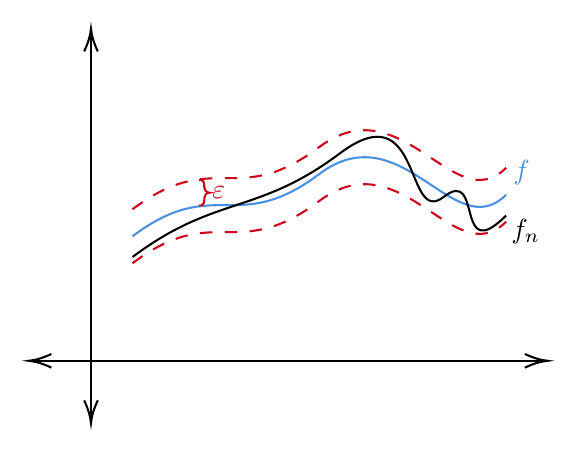
\begin{tikzpicture}[x=0.75pt,y=0.75pt,yscale=-1,xscale=1]
    %uncomment if require: \path (0,300); %set diagram left start at 0, and has height of 300
    
    %Straight Lines [id:da15070589522945865] 
    \draw    (120,42) -- (120,228) ;
    \draw [shift={(120,230)}, rotate = 270] [color={rgb, 255:red, 0; green, 0; blue, 0 }  ][line width=0.75]    (10.93,-3.29) .. controls (6.95,-1.4) and (3.31,-0.3) .. (0,0) .. controls (3.31,0.3) and (6.95,1.4) .. (10.93,3.29)   ;
    \draw [shift={(120,40)}, rotate = 90] [color={rgb, 255:red, 0; green, 0; blue, 0 }  ][line width=0.75]    (10.93,-3.29) .. controls (6.95,-1.4) and (3.31,-0.3) .. (0,0) .. controls (3.31,0.3) and (6.95,1.4) .. (10.93,3.29)   ;
    %Straight Lines [id:da06812433005878815] 
    \draw    (338,200) -- (92,200) ;
    \draw [shift={(90,200)}, rotate = 360] [color={rgb, 255:red, 0; green, 0; blue, 0 }  ][line width=0.75]    (10.93,-3.29) .. controls (6.95,-1.4) and (3.31,-0.3) .. (0,0) .. controls (3.31,0.3) and (6.95,1.4) .. (10.93,3.29)   ;
    \draw [shift={(340,200)}, rotate = 180] [color={rgb, 255:red, 0; green, 0; blue, 0 }  ][line width=0.75]    (10.93,-3.29) .. controls (6.95,-1.4) and (3.31,-0.3) .. (0,0) .. controls (3.31,0.3) and (6.95,1.4) .. (10.93,3.29)   ;
    %Curve Lines [id:da9975807479144934] 
    \draw [color={rgb, 255:red, 74; green, 144; blue, 226 }  ,draw opacity=1 ]   (140,140) .. controls (180,110) and (190,140) .. (230,110) .. controls (270,80) and (295,145) .. (320,120) ;
    %Curve Lines [id:da8386196196350342] 
    \draw [color={rgb, 255:red, 208; green, 2; blue, 27 }  ,draw opacity=1 ] [dash pattern={on 4.5pt off 4.5pt}]  (140,127) .. controls (180,97) and (190,127) .. (230,97) .. controls (270,67) and (295,132) .. (320,107) ;
    %Curve Lines [id:da7136000427009845] 
    \draw [color={rgb, 255:red, 208; green, 2; blue, 27 }  ,draw opacity=1 ] [dash pattern={on 4.5pt off 4.5pt}]  (140,153) .. controls (180,123) and (190,153) .. (230,123) .. controls (270,93) and (295,158) .. (320,133) ;
    %Shape: Brace [id:dp021850826872210183] 
    \draw  [color={rgb, 255:red, 208; green, 2; blue, 27 }  ,draw opacity=1 ] (172,125.25) .. controls (173.71,125.25) and (174.57,124.39) .. (174.57,122.68) -- (174.57,122.68) .. controls (174.57,120.23) and (175.43,119) .. (177.15,119) .. controls (175.43,119) and (174.57,117.77) .. (174.57,115.32)(174.57,116.43) -- (174.57,115.32) .. controls (174.57,113.61) and (173.71,112.75) .. (172,112.75) ;
    %Curve Lines [id:da39763918210258864] 
    \draw    (140,150) .. controls (180,120) and (200,130) .. (240,100) .. controls (280,70) and (271,135.75) .. (290,121) .. controls (309,106.25) and (295,155) .. (320,130) ;
    
    % Text Node
    \draw (177,119) node [anchor=west] [inner sep=0.75pt]  [color={rgb, 255:red, 208; green, 2; blue, 27 }  ,opacity=1 ]  {$\varepsilon $};
    % Text Node
    \draw (322,116.6) node [anchor=south west] [inner sep=0.75pt]  [color={rgb, 255:red, 74; green, 144; blue, 226 }  ,opacity=1 ]  {$f$};
    % Text Node
    \draw (321,130.4) node [anchor=north west][inner sep=0.75pt]  [color={rgb, 255:red, 0; green, 0; blue, 0 }  ,opacity=1 ]  {$f_{n}$};
    
    
    \end{tikzpicture}
    

\end{center}


Equivalently, we could say that for all $\varepsilon > 0$ there's some $N \in \N$ such that for all $n \geq N$ we have $\sup_{x \in S} |f_n(x) - f(x)| < \varepsilon$.

The above definition implies that if we fix some value of $x$ that $f_1(x), f_2(x), \dots$ converges to $f(x)$. This implies that the function $f$ is unique, due to the uniqueness of limits in $\R$ and $\C$. We sometimes call $f$ the \vocab{uniform limit}.

\begin{definition}[Pointwise Convergence]
We say that $f_n$ \vocab{converges pointwise} on $S$ to $f$ if $f_n(x) \rightarrow f(x)$ for every $x \in S$.
\end{definition}
\begin{remark}
    In this definition our `$N$' can depend on $\varepsilon$ \emph{and} $x$! This makes it a much weaker notion than uniform convergence, and clearly uniform convergence implies pointwise convergence.
\end{remark}

\begin{example}[Checking Uniform Convergence]
    Consider the sequence of functions $f_n(x) = x^2 \cdot e^{-n x}$ for $n \in \N$ and $x \in \R^+$. We want to know if this sequence of functions converges uniformly on this domain.

    Since pointwise convergence is implied by uniform convergence, we can first check the pointwise limit exists and use that to specify $f$ in our definition of uniform convergence.

    Fix $x \geq 0$. Then $x^2 e^{-nx} \rightarrow 0$ as $n \rightarrow \infty$. So $f_n$ tends to $0$ (the zero function) pointwise on $\R^+$. We can now check if $f_n$ converges uniformly to the zero function.

    We can attempt to compute the quantity
    $$
    \sup_{x \geq 0} |f_n(x) - 0| =  \sup_{x \geq 0} f_n(x).
    $$
    One approach would be to differentiate it, which would need some care. A better way is to find an upper bound on $|f_n(x) - f(x)|$ which does not depend on $x$. In this case we can bound
    $$
    0 \leq x^2 e^{-nx} = \frac{x^2}{1 + nx + n^2x^2/2 + \cdots} \leq \frac{2}{n^2},
    $$
    for all $x \geq 0$. Thus $\sup_{x \geq 0} f_n(x) \leq 2/n^2 \rightarrow 0$ as $n \rightarrow \infty$. So indeed $f_n \rightarrow 0$ uniformly on $\R^+$.
\end{example}

\begin{example}[Showing Uniform Convergence Doesn't Hold]
    Consider the sequence of functions $f_n(x) = x^n$ for $n \in \N$, over the domain $[0, 1]$.

    We can compute the limit as
    $$
    x^n \rightarrow f(x) = \begin{cases}
        0 &\mbox{if } 0 \leq x < 1, \\
        1 &\mbox{if } x = 1.
       \end{cases}
    $$
    This implies that $\sup_{x \in [0, 1]} |f_n(x) - f(x)| = 1$. So this doesn't tend to zero, and thus the sequence of functions $f_n$ converges pointwise but not uniformly.

    \begin{center}
    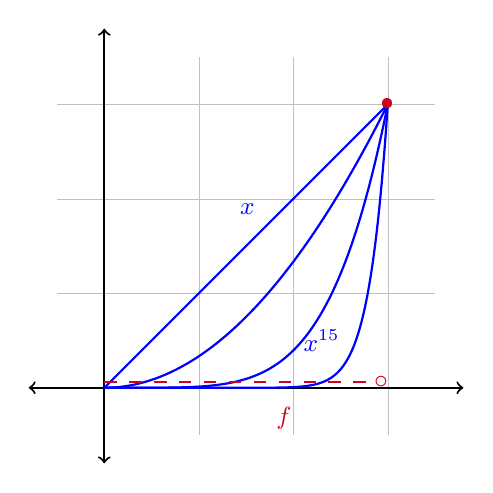
\begin{tikzpicture}[scale=1.2]
        \draw[ultra thin, color=lightgray] (-0.5,-0.5) grid (3.5,3.5);
        \draw[<->] (-0.8,0) -- (3.8,0);
        \draw[<->] (0,-0.8) -- (0,3.8);
        \draw[thick, samples=100, smooth, domain=0:3, color=blue] plot (\x, {3*(\x/3)});
        \draw[thick, samples=100, smooth, domain=0:3, color=blue] plot (\x, {3*((\x/3)^2)});
        \draw[thick, samples=100, smooth, domain=0:3, color=blue] plot (\x, {3*((\x/3)^5)});
        \draw[thick, samples=150, smooth, domain=0:3, color=blue] plot (\x, {3*((\x/3)^(15))});
        \draw[dash pattern={on 4.5pt off 4.5pt}, color={rgb,255:red,208;green,2;blue,27}] (0,0.06) -- (2.85,0.06);
        \node[color={rgb,255:red,208;green,2;blue,27}] at (2.93,0.06) {$\circ$};
        \node[color={rgb,255:red,208;green,2;blue,27}] at (3,3) {\textbullet};
        \node[color={rgb,255:red,208;green,2;blue,27}, anchor=north] at (1.9,-0.1) {\small $f$};
        \node[color=blue, anchor=south east] at (1.7,1.72) {\small $x$};
        \node[color=blue, anchor=east] at (2.6,0.5) {\small $x^{15}$};
    \end{tikzpicture}
    \end{center}

    The picture above shows what is going wrong -- as $n$ grows, the graph of $x^n$ sags towards zero, but it always has to climb back up to $1$ at the right endpoint. The convergence near $x = 1$ is genuinely slower, and no single $N$ works across the whole interval.

    Alternatively, we could compute $\sup_{x \in [0, 1]} f_n(x) \geq f_n((1/2)^{1/n}) = 1/2$, which shows that $f_n$ does not converge uniformly.
\end{example}

\begin{remark}
    The statement ``$f_n \not \rightarrow f$ uniformly on the domain $S$'' means there exists some $\varepsilon$ such that for all $N \in \N$, there's some $n \geq N$ and $x \in S$ such that $|f_n(x) - f(x)| \geq \varepsilon$. In many cases when thinking about this, it's almost easier just to negate the statement symbolically.
\end{remark}

We will now see that the uniform limit function retains certain properties from the original sequence. For example, the uniform limit of continuous functions is continuous.

\begin{theorem}[Continuity of the Uniform Limit]
    Let $S \subseteq \R$ or $\C$. Given a sequence of functions $f_n : S \rightarrow \R$ (or $\C$), if $f_n$ is continuous for all $n$, and $f_n \rightarrow f$ uniformly on $S$, then $f$ is continuous.
\end{theorem}
\begin{proof}
    We will show that $f$ is continuous at some arbitrary $a \in S$. Given $\varepsilon > 0$, there exists some $n \in \N$ such that for $x \in S$ we have $|f_n(x) - f(x)| < \varepsilon /3$. Then since $f_n$ is continuous, there exists $\delta > 0$ such that $|x - a| < \delta$ implies that $|f_n(x) - f_n(a)| < \varepsilon / 3$. Then if $x \in S$ and $|x - a| < \delta$, we have
    $$
    |f(x) - f(a)| \leq |f(x) - f_n(x)| + |f_n(x) - f_n(a)| + |f_n(a) - f(a)| \leq \varepsilon,
    $$
    as required\footnote{This type of proof is called a `$\varepsilon/3$' proof, or a $3 \varepsilon$ proof depending on your outlook}.
\end{proof}

\begin{remark}
    This result \emph{does not} hold for just pointwise convergence. For example, consider $f_n(x) = x^n$ on the interval $[0, 1]$. However, the set of points at which it can be discontinuous is relatively small. Also this result does not hold for differentiability.
\end{remark}

Another way of viewing this result is that it gives us a case where swapping limits is okay\footnote{Generally, swapping limits is bad.}, that is 
$$
    \lim_{x \to a} \lim_{n \to \infty} f_n(x) = \lim_{x \to a} f(x) = f(a),
$$
if $f_n$ converges uniformly to $f$.

We can also prove that boundedness is a property preserved by the uniform limit.

\begin{lemma}[Uniform Limit of Bounded Functions is Bounded]\label{lemma:uniform-bounded}
Assume that $f_n \rightarrow f$ uniformly on some set $S$.  
If $f_n$ is bounded for every $n$, then so is $f$.  
\end{lemma}
\begin{proof}
Fix some $n \in \N$ such that for all $x \in S$ we have $|f_n(x) - f(x)| < 1$. Then since $f_n$ is bounded, there is an $M \in \R$ such that $|f_n(x)| \leq M$ for all $x \in S$. Thus
$$
    |f(x)| \leq |f(x) - f_n(x)| + |f_n(x)| \leq 1 + M,
$$
so $f$ is bounded.
\end{proof}

Another natural property that's preserved by the uniform limit is integrability. Since we have $f$ bounded, we can sensibly talk about the upper and lower sums, and just need to check that Riemann's criterion is satisfied.

% You may recall from a previous analysis course that if $f:[a, b] \rightarrow \R$ is bounded, then for a dissection $\DD = \{x_0, x_1, \dots, x_n\}$ with $a = x_0 \leq x_1 \leq \cdots \leq x_n = b$, we can define the upper and lower sums of $f$ with respect to $\DD$ as
% \begin{align*}
%     S_{\DD}(f) &= \sum_{j = 1}^n (x_j - x_{j - 1}) \sup_{x \in [x_{j - 1}, x_j]} f(x), \\
%     s_{\DD}(f) &= \sum_{j = 1}^n (x_j - x_{j - 1}) \inf_{x \in [x_{j - 1}, x_j]} f(x).
% \end{align*}
% With this we have Riemann's criterion for integrability, which is that a function is integrable if and only if for all $\varepsilon > 0$ there exists some dissection $\DD$ such that $S_{\DD}(f) - s_{\DD}(f) < \varepsilon$.

% It's easy to see that for any $I \subset [a, b]$
% $$
% \sup_{I} f - \inf_I f = \sup_{x, y \in I} (f(x) - f(y)) = \sup_{x, y \in I} |f(x) - f(y)|.
% $$
% This is called the \vocab{oscillation} of $f$ on $I$, and the integrability criterion above says that integrable functions don't oscillate too much.

\begin{theorem}[Uniform Limit of Integrable Functions is Integrable]\label{thm3}
Let $f_n: [a, b] \rightarrow \R$ be a sequence of integrable functions. If $f_n \rightarrow f$ uniformly on $[a, b]$ then $f$ is integrable and
$$
\int_a^b f_n \rightarrow \int_a^b f,
$$
as $n \rightarrow \infty$.
\end{theorem}
\begin{proof}
    Since every $f_n$ is integrable, they must all be bounded and hence $f$ is also bounded. Thus it suffices to check that Riemann's criterion is satisfied.

    Given $\varepsilon > 0$, we can fix an $n \in \N$ such that $x \in [a, b]$ implies $|f_n(x) - f(x)| < \varepsilon$. Then since $f_n$ is integrable, there exists a dissection $\DD = \{x_0, x_1, \dots, x_m\}$ of $[a, b]$ such that $S_{\DD}(f_n) - s_{\DD}(f_n) < \varepsilon$. 

    Now, for each $k \in \{1, \dots, m\}$ and any $x,y \in[x_{k - 1}, x_k]$, we have
    \begin{align*}
        |f(x) - f(y)| &\leq |f(x) - f_n(x)| + |f_n(x) - f_n(y)| + |f_n(y) - f(y)| \\
        &\leq |f_n(x) - f_n(y)| + 2 \varepsilon.
    \end{align*}
    Then noting that we can write the difference between the supremum and infimum of $f$ in the interval $[x_{k - 1}, x_k]$ as
    $$
        \sup_{x, y \in [x_{k - 1}, x_k]} |f(x) - f(y)| \leq \sup_{x, y \in [x_{k - 1}, x_k]} |f_n(x) - f_n(y)| + 2 \varepsilon,
    $$
    we can multiply by $(x_k - x_{k - 1})$ and sum over $k$ to get 
    $$ 
    S_{\DD}(f) - s_{\DD}(f) \leq S_{\DD}(f_n) - s_{\DD}(f_n) + 2 \varepsilon (b - a) \leq \varepsilon (2(b - a) + 1),
    $$
    so $f$ is integrable.

    Finally, we can write
    $$
    \left|\int_a^b f_n - \int_a^b f\right| \leq \int_a^b |f_n - f| \leq (b - a) \cdot \sup_{[a, b]} |f_n - f| \rightarrow 0
    $$
    as $n \rightarrow \infty$.
\end{proof}

Similar to the previous theorem, this result can be viewed as giving us a case where swapping integrals (which are some form of limit) and limits is okay, so that
$$
    \int_a^b \lim_{n \to \infty} f_n(x) \dd x = \lim_{n \to \infty} \int_a^b f_n(x) \dd x,
$$
whenever $f_n \rightarrow f$ uniformly.


From these results\footnote{The derivation is straightforward, just consider the sequence of partial sums!}, we obtain some results on how we can both integrate and differentiate sufficiently nice functions term by term.

\begin{theorem}[Term-wise Integration]
    Let $g_n: [a, b] \rightarrow \R$ be a sequence of integrable functions. Then if $\sum_{n = 1}^{\infty} g_n(x)$ converges uniformly on $[a, b]$, the function $x \mapsto \sum_{n = 1}^{\infty} g_n(x)$ is integrable and
    $$
    \int_a^b \sum_{n = 1}^{\infty} g_n(x) \dd x = \sum_{n = 1}^{\infty} \int_a^b g_n(x) \dd x.
    $$
\end{theorem}
\begin{proof}[Proof Sketch]
    Let $f_n$ be the sequence of partial sums, and notice that $f_n$ converging uniformly implies that we can apply the previous theorem.
\end{proof}

\begin{theorem}[Term-wise Differentiation]
    Let $g_n: [a, b] \rightarrow \R$ be a sequence of continuously differentiable functions. If $\sum_{j = 1}^n g_j(c)$ converges for \emph{some} $c \in [a, b]$ and $\sum_{j = 1}^n g'_j$ converges uniformly as $n \rightarrow \infty$, then $\sum_{j = 1}^{\infty} g_j$ converges uniformly to a continuously differentiable function $g$, and
    $$
   g'(x) = \frac{\dd}{\dd x} \left(\sum_{j = 1}^{\infty} g_j(x)\right) = \sum_{j = 1}^{\infty} g'_j(x).
    $$
\end{theorem}
\begin{proof}
    We are going to try and solve $g' = h$, where we let $h(x) = \sum_{k = 1}^{\infty} g'_k(x)$, subject to the initial condition $g(c) = \sum_{n = 1}^{\infty} g_n(c)$.

    Since $\sum_{n = 1}^{\infty} g_n'(x)\rightarrow h$ uniformly, and since $g_n'$ is continuous, we know that $h$ is continuous and thus integrable. 

    Now let $\lambda = \sum_{n = 1}^{\infty} g_n(c)$, and define
    $$
    g(x) = \lambda + \int_c^x h(t) \dd t,
    $$
    for $x \in [a, b]$. Since $h$ is continuous, by the fundamental theorem of calculus, $g$ is differentiable with $g' = h$, and moreover, $g(c) = \lambda$.

    Again by the fundamental theorem of calculus, we also have
    $$
    g_k(x) = g_k(c) + \int_c^x g_k'(t) \dd t,
    $$
    for $x \in [a, b]$ and $k \in \N$. 

    Now given $\varepsilon > 0$, there exists a positive integer $N$ such that for $n \geq N$ we have
    $$
    \left|\lambda - \sum_{k = 1}^n g_k(c)\right| < \frac{\varepsilon}{2}, \quad \text{and} \quad \left|h(t) - \sum_{k = 1}^n g_k'(t)\right| < \frac{\varepsilon}{2(b - a)},
    $$
    for $t \in [a, b]$. Then for $x \in [a, b]$, we have
    \begin{align*}
        \left|g(x) - \sum_{k = 1}^n g_k(x)\right| &= 
        \left|\lambda + \int_c^x h(t)\dd t - \sum_{k = 1}^n \left(g_k(c) + \int_c^x g_k'(t) \dd t \right)\right|
        \\
        & \leq \left|\lambda - \sum_{k = 1}^n g_k(c)\right| + \left|\int_c^x \left(h(t) - \sum_{k = 1}^n g_k'(t) \right) \dd t\right| \\
        &\leq \frac{\varepsilon}{2} + |x - c| \cdot \frac{\varepsilon}{2(b - a)} \\&\leq \varepsilon.
    \end{align*}
    This shows that $\sum_{k = 1}^n g_k(x) \rightarrow g(x)$ uniformly on $[a, b]$, and we also know that $g$ is differentiable and $g' = h$ is continuous.
\end{proof}

\subsection{The General Principle of Uniform Convergence}

If a sequence $x_n \in \R$ is Cauchy, that is, if for all $\varepsilon > 0$ there exists a positive integer $N$ such that $m, n \geq N$ implies $|x_m - x_n| < \varepsilon$, then the \emph{general principle of convergence} says that the sequence converges.
Said differently, terms in a sequence getting arbitrarily close together is necessary and sufficient for convergence. 

A similar concept can be applied to sequences of functions.

\begin{definition}[Uniformly Cauchy]
    A sequence $f_n$ of functions on a set $S$ is \vocab{uniformly Cauchy} if for all $\varepsilon > 0$ there exists a positive integer $N$ such that $n, m \geq N$ implies that for any $x \in S$ we have $|f_m(x) - f_n(x)| < \varepsilon$.
\end{definition}

From this, we get an analogue of the general principle of convergence for uniform convergence.

\begin{theorem}[General Principle of Uniform Convergence]
    If $f_n$ is a uniformly Cauchy sequence of functions on a set $S$, then it converges uniformly on $S$ to some function $f$.
\end{theorem}
\begin{proof}
    For any $x \in S$, the sequence of functions being uniformly Cauchy implies that the sequence of reals $f_n(x)$ is Cauchy. Thus $f_n(x)$ converges for all $x \in S$, and $f_n$ converges pointwise to some function $f$. 

    Given $\varepsilon > 0$, there is some positive integer $N$ such that for all $m, n \geq N$ and all $x \in S$, $|f_m(x) - f_n(x)| < \varepsilon/2$. We first fix $x \in S$, and fix $n \geq N$. Since $f_m(x) \rightarrow f(x)$ as $m \rightarrow \infty$, we can choose $m \in \N$ such that $|f_m(x) - f(x)| < \varepsilon/2$, and $m \geq N$. Then
    $$
    |f_n(x) - f(x)| \leq |f_n(x) - f_m(x)| + |f_m(x) - f(x)| < \varepsilon,
    $$
    as required, and thus $f_n$ converges uniformly to $f$.
\end{proof}

% Alternative end of proof from 'fix x in S', we can do |f_n(x) - f_m(x)| < epsilon for all m >= N, then let m -> infty.

This is an incredibly important theorem, and has lots of applications. One example is proving the uniform convergence of certain power series, which we will see below.

\begin{theorem}[Weierstrass $M$-test]
    Let $f_n$ be a sequence of functions on a set $S$. Assume that for every $n \in \N$ there is an $M_n \in \R^+$ such that $|f_n(x)| \leq M_n$ for all $x \in S$. If $\sum_{n = 1}^{\infty} M_n$ converges, then $\sum_{n = 1}^{\infty} f_n(x)$ converges uniformly on $S$.
\end{theorem}
\begin{proof}
    Let $F_n(x) = \sum_{k = 1}^n f_k(x)$ where $x \in S$ and $n \in \N$.
    For $x \in S$ and $n \geq m$ we have
    $$
    |F_n(x) - F_m(x)| \leq \sum_{k = m + 1}^n |f_k(x)| \leq \sum_{k = m + 1}^n M_k.
    $$
    Now given $\varepsilon>0$, we can choose $N \in \N$ such that $\sum_{k = N + 1}^{\infty} M_k < \varepsilon$. Then for every $x \in S$ and $n \geq m \geq N$, we have
    $$
    |F_n(x) - F_m(x)| \leq \sum_{k = m + 1}^{\infty} M_k < \varepsilon,
    $$
    so $F_n$ is uniformly Cauchy on $S$, and hence converges uniformly on $S$ by the general principle of uniform convergence.
\end{proof}

\begin{definition}[Open Disk]
    We define the \vocab{complex open disk} $D(a, R)$ to be the set 
    $$
    D(a, R) = \{ z \in \C \mid |z - a| < R \}.
    $$
\end{definition}

\begin{example}[Uniform Convergence of $\sum_{n = 1}^{\infty} z^n/n^2$]
    We want to know if the power series $\sum_{n = 1}^{\infty} z^n/n^2$ converges uniformly.

    It's easy to check that the radius of convergence is $1$, so now we consider the terms in the sequence $f_n(z) = z^n/n^2$ where $z \in D(0, 1)$.

    For all such $z$, $|f_n(z)| \leq 1/n^2$, and since $\sum_{n = 1}^{\infty} 1/n^2$ is convergent, by the $M$-test, this power series converges uniformly on $D(0, 1)$.
\end{example}

Of course, not every power series converges uniformly. 

For example, the power series $\sum_{n = 0}^{\infty} z^n$ has radius of convergence $1$, and has bounded partial sums for $z \in D(0, 1)$. However, it converges to $1/(1 - z)$, which is not bounded (and hence the convergence can't be uniform, as otherwise boundedness would be preserved).

Despite this example, we can see that uniform convergence basically failed near the radius of convergence, and we can still recover a nice result if we just move \emph{slightly} away, we can still get uniform convergence.

\begin{theorem}[Uniform Convergence Near the Radius of Convergence]
    Assume the power series $\sum_{n = 0}^{\infty} c_n (z - a)^n$ has radius of convergence $R$. Then for any $r$ with $0 < r < R$, the power series converges uniformly on $D(a, r)$.
\end{theorem}
\begin{proof}
    Fix some $w \in \C$ such that $r < |w - a| < R$. We set $\rho = \frac{r}{|w - a|}$, and we note that $\rho \in (0, 1)$. 

    Since $\sum_{n = 0}^{\infty} c_n(w - a)^n$ converges, we have $c_n(w - a)^n \rightarrow 0$ as $n \rightarrow \infty$. Thus there exists some $M \in \R^+$ such that $|c_n(w - a)^n| \leq M$ for all $n \in \N$.

    Now if we take $z \in D(a, r)$ and $n \in \N$, we have
    \begin{align*}
        |c_n(z - a)^n| &= |c_n (w - a)^n| \cdot \left(\frac{|z - a|}{|w - a|}\right)^n \\
        &\leq M \left(\frac{r}{|w - a|}\right)^n \leq M \rho^n.
    \end{align*}
    Then since $\sum_{n = 0}^{\infty} M \rho^n$ is convergent, by the $M$-test we have $\sum_{n = 0}^{\infty} c_n(z - a)^n$ converging uniformly for $z \in D(a, r)$.
\end{proof}

This result allows us to use our results about uniform convergence to say things about power series. For example:

\begin{enumerate}
    \item Since a power series is the uniform limit of polynomials inside the radius of convergence, and polynomials are continuous, we get that power series are also continuous inside their radius of convergence.
    \item Using our term-wise differentiability result, we get that power series can be differentiated term-wise inside their radius of convergence, and that the power series $\sum_{n = 0}^{\infty} c_n(z - a)^n$ has derivative $\sum_{n = 1}^{\infty} c_n \cdot n (z - a)^{n - 1}$. 
\end{enumerate} 

We saw previously that it's possible for a power series to not converge uniformly on its whole open disk of convergence. However, the previous theorem showed that we could get arbitrarily close to the radius of convergence, and we'd still have \emph{some} amount of uniform convergence.

To be exact, consider a power series $\sum_{n = 0}^{\infty} c_n(z - a)^n$ with radius of convergence $R$. Then if we take some $w \in D(a, R)$, and fix some $r$ such that $|w - a| < r < R$, we can find some $\delta > 0$ such that $|w - a| + \delta < r$.

\begin{center}
    

\tikzset{every picture/.style={line width=0.75pt}} %set default line width to 0.75pt        

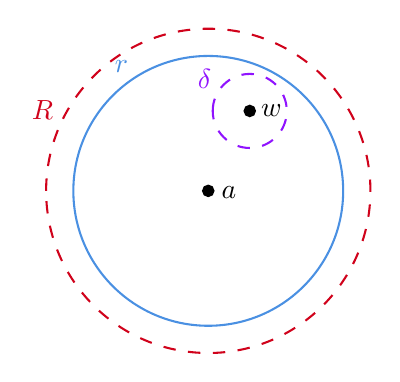
\begin{tikzpicture}[x=0.75pt,y=0.75pt,yscale=-1,xscale=1]
%uncomment if require: \path (0,300); %set diagram left start at 0, and has height of 300

%Shape: Circle [id:dp18825895148913352] 
\draw  [color={rgb, 255:red, 208; green, 2; blue, 27 }  ,draw opacity=1 ][dash pattern={on 4.5pt off 4.5pt}] (174.38,97.5) .. controls (174.38,54.35) and (209.35,19.38) .. (252.5,19.38) .. controls (295.65,19.38) and (330.63,54.35) .. (330.63,97.5) .. controls (330.63,140.65) and (295.65,175.62) .. (252.5,175.62) .. controls (209.35,175.62) and (174.38,140.65) .. (174.38,97.5) -- cycle ;
%Shape: Circle [id:dp8728584687593086] 
\draw  [fill={rgb, 255:red, 0; green, 0; blue, 0 }  ,fill opacity=1 ] (250,97.5) .. controls (250,96.12) and (251.12,95) .. (252.5,95) .. controls (253.88,95) and (255,96.12) .. (255,97.5) .. controls (255,98.88) and (253.88,100) .. (252.5,100) .. controls (251.12,100) and (250,98.88) .. (250,97.5) -- cycle ;
%Shape: Circle [id:dp10489496235227858] 
\draw  [color={rgb, 255:red, 74; green, 144; blue, 226 }  ,draw opacity=1 ] (187.5,97.5) .. controls (187.5,61.6) and (216.6,32.5) .. (252.5,32.5) .. controls (288.4,32.5) and (317.5,61.6) .. (317.5,97.5) .. controls (317.5,133.4) and (288.4,162.5) .. (252.5,162.5) .. controls (216.6,162.5) and (187.5,133.4) .. (187.5,97.5) -- cycle ;
%Shape: Circle [id:dp9134235647013942] 
\draw  [fill={rgb, 255:red, 0; green, 0; blue, 0 }  ,fill opacity=1 ] (270,59) .. controls (270,57.62) and (271.12,56.5) .. (272.5,56.5) .. controls (273.88,56.5) and (275,57.62) .. (275,59) .. controls (275,60.38) and (273.88,61.5) .. (272.5,61.5) .. controls (271.12,61.5) and (270,60.38) .. (270,59) -- cycle ;
%Shape: Circle [id:dp2734402369917359] 
\draw  [color={rgb, 255:red, 144; green, 19; blue, 254 }  ,draw opacity=1 ][dash pattern={on 4.5pt off 4.5pt}] (254.66,59) .. controls (254.66,49.15) and (262.65,41.16) .. (272.5,41.16) .. controls (282.35,41.16) and (290.34,49.15) .. (290.34,59) .. controls (290.34,68.85) and (282.35,76.84) .. (272.5,76.84) .. controls (262.65,76.84) and (254.66,68.85) .. (254.66,59) -- cycle ;

% Text Node
\draw (257.5,98.5) node [anchor=west] [inner sep=0.75pt]    {$a$};
% Text Node
\draw (166,52.4) node [anchor=north west][inner sep=0.75pt]  [color={rgb, 255:red, 208; green, 2; blue, 27 }  ,opacity=1 ]  {$R$};
% Text Node
\draw (206,33.4) node [anchor=north west][inner sep=0.75pt]  [color={rgb, 255:red, 74; green, 144; blue, 226 }  ,opacity=1 ]  {$r$};
% Text Node
\draw (276.5,59) node [anchor=west] [inner sep=0.75pt]    {$w$};
% Text Node
\draw (246,37.4) node [anchor=north west][inner sep=0.75pt]  [color={rgb, 255:red, 144; green, 19; blue, 254 }  ,opacity=1 ]  {$\delta $};


\end{tikzpicture}

\end{center}

Then if $|z - w| < \delta$, $|z - a| \leq |z - w| + |w - a| < \delta + |w - a| < r$, so $D(w, \delta) \subset D(a, r)$, and thus $\sum_{n =0}^{\infty} c_n (z - a)^n$ converges uniformly on $D(w, \delta)$.

This inspires a helpful definition.

\begin{definition}[Open]
    A subset $U$ of $\C$ is \vocab{open} if for all $w \in U$ there exists $\delta > 0$ such that $D(w, \delta) \subset U$.
\end{definition}

\begin{definition}[Local Uniform Convergence]
    Let $U$ be an open subset of $\C$ and $f_n$ be a sequence of functions on $U$. We say that $f_n$ \vocab{converges locally uniformly} on $U$ if for all $w \in U$ there exists some $\delta > 0$ such that $f_n$ converges uniformly on $D(w, \delta) \subset U$.  
\end{definition}

With this the result we discussed above can be stated as follows.

\begin{theorem}[Local Uniform Convergence of Power Series]
    A power series centered at $a$ with radius of convergence $R$ converges locally uniformly on $D(a, R)$.
\end{theorem}

We will return to this when we discuss compactness later on.

\subsection{Uniform Continuity}

Recall the standard notion of continuity.

\begin{definition}[Continuity]
	Let $A \subseteq \C$ and $f: A \rightarrow \C$. We say that $f$ is \vocab{continuous at $a$} $\in A$ if given any $\epsilon > 0$ we can find a $\delta > 0$ such that $|f(a) - f(x)| < \epsilon$ for all $x \in A$ such that $|x -a | < \delta$.


	We say that $f$ is \vocab{continuous} if it is continuous at every $a \in A$.
\end{definition}

In the above definition, our $\delta$ is allowed to depend on both $\varepsilon$ \emph{and} $x$.

\begin{definition}[Uniform Continuity]
    Let $A \subset \C$ and $f: A \rightarrow \C$. We say that $f$ is \vocab{uniformly continuous} on $A$ if given any $\varepsilon > 0$ we can find a $\delta > 0$ such that for all $x, y \in A$ we have $|x - y| < \delta$ implying $|f(x) - f(y)| < \varepsilon$.
\end{definition}

Here, we again impose this \emph{uniformity} constraint, that is, $\delta$ is allowed to depend on $\varepsilon$ only. 

It's easy to see that uniform continuity implies continuity, but the converse doesn't hold in general.

\begin{example}[Uniformly Continuous Function]
    We will show that $f(x) = 2x + 17$ is uniformly continuous over $\R$. 

    Given $\varepsilon > 0$, let $\delta = \varepsilon / 2$. Then for all $x, y \in \R$ with $|x - y| < \delta$ we have $|f(x) - f(y)| = 2|x - y| < \varepsilon$, as required.
\end{example}

\begin{example}[A Non-Uniformly Continuous Function]
    The function $f(x) = x^2$ over $\R$ is continuous, but not uniformly continuous. 

    Consider $\varepsilon = 1$. Then given some $\delta$, let $x = 1/\delta$ and $y = 1/\delta + \delta/2$. Then we have $|x - y| < \delta$ but $|f(x) - f(y)| = 1 + \delta^2/4 > 1 = \varepsilon$, so $f$ is not uniformly continuous.
\end{example}

Here, our uniform continuity was shown to not hold by taking larger and larger $x$, which forced the slope of the function to get too large for a given value of $\delta$ to be sufficient. It turns out that this is the only failure point of uniform continuity, and indeed continuity implies uniform continuity when we are working over a bounded interval.

The proof of this is quite natural -- we use Bolzano-Weierstrass to show that a contradiction to uniform continuity is a contradiction to continuity.\footnote{Another argument which is more direct can be made using compactness, but we will look past this for now.}

\begin{theorem}[Continuous Functions are Uniformly Continuous]
    Let $f: [a, b] \rightarrow \C$ be continuous. Then $f$ is uniformly continuous.
\end{theorem}
\begin{proof}
	Suppose $f$ was not uniformly continuous, that is, there exists some $\epsilon > 0$ such that for all $\delta > 0$ there is some $x, y$ with $|x - y| < \delta$ such that $|f(x) - f(y)| \geq \epsilon$.

	Taking $\delta = 1/n$, we can find some sequences $x_n, y_n \in [a, b]$ such that $|x_n - y_n| < 1/n$, and $|f(x_n) - f(y_n)| \geq \epsilon$. Then by Bolzano-Weierstrass, we can find some convergent subsequence $x_{n_j} \rightarrow x$ for some $x \in [a, b]$. But then $|x_{n_j} - y_{n_j}| < 1/n_j$ for all $j$, so we must have $y_{n_j} \rightarrow x$ also.

	Then $|f(x_{n_j}) - f(y_{n_j})| \geq \epsilon$ for every $j$, which implies that $f(x_{n_j})$ and $f(y_{n_j})$ cannot converge to the same value. But then by continuity we have $f(x_{n_j}) \rightarrow f(x)$ and $f(y_{n_j}) \rightarrow f(x)$, which is a contradiction. Thus $f$ must be uniformly continuous.
\end{proof}

With this result, we can prove the familiar result that continuous functions are integrable.

\begin{theorem}[Continuous Functions are Integrable]
	Let $f:[a, b] \rightarrow \R$ be continuous. Then $f$ is Riemann integrable.
\end{theorem}
\begin{proof}
	Given $\epsilon > 0$, since $f$ is uniformly continuous, there is some $\delta > 0$ such that $|f(x) - f(y)| < \epsilon/(b - a)$ whenever $|x - y| < \delta$ and $x, y \in [a, b]$.

	Now choose some integer $n$ large enough that $(b - a)/n < \delta$, and define the dissection $\DD = \{x_0, x_1, \dots, x_n\}$ with $x_j = a + j(b - a)/n$. Then we have
	$$
	\sup_{x \in [x_{j - 1}, x_j]} f(x) - \inf_{x \in [x_{j - 1}, x_j]} f(x) \leq \frac{\epsilon}{(b - a)},
	$$
	for all $1 \leq j \leq n$, and thus 
	\begin{align*}
		S_\DD(f) - s_\DD(f) &= \sum_{j = 1}^n (x_j - x_{j - 1})\left[\sup_{x \in [x_{j - 1}, x_j]} f(x) - \inf_{x \in [x_{j - 1}, x_j]} f(x)\right] \\
		&\leq \sum_{j = 1}^n \frac{b - a}{n} \cdot \frac{\epsilon}{b - a} = \epsilon,
	\end{align*}
	and thus $f$ is Riemann integrable.
\end{proof}

\section{Metric Spaces}

\subsection{Defining Metric Spaces}

In $\R$ and $\C$, we measured the `closeness' of two points $x, y$ using $|x - y|$. We used this throughout our study of analysis both in this course and previously, and possibly the most important property of this was the triangle inequality,
$$
|x - z| \leq |x - y| + |y - z|.
$$

The triangle inequality acts, more or less, as saying that being close is \emph{transitive}. That is, if $x$ is close to $y$, and $y$ is close to $z$, then $x$ is close to $z$.

In fact, we can abstract away quite naturally from the absolute value into a more general setting in which a measure of distance has this property.

\begin{definition}[Metric]
    Let $M$ be a set. A \vocab{metric} on $M$ is a function $d: M \times M \rightarrow \R$ such that
    \begin{itemize}
        \item \emph{Positivity}. For all $x, y \in M$, $d(x, y) \geq 0$, with equality if and only if $x = y$.
        \item \emph{Symmetry}. For all $x, y \in M$, $d(x, y) = d(y, x)$.
        \item \emph{Triangle inequality}. For all $x, y, z \in M$,
        $$
        d(x, z) \leq d(x, y) + d(y, z).
        $$
    \end{itemize}
\end{definition}

\begin{definition}[Metric Space]
    A \vocab{metric space} is a pair $(M, d)$ where $M$ is a set and $d$ is a metric on $M$. 
\end{definition}

\begin{example}[Metric Spaces on $\R$]
    The real line $\R$ is a metric space under the metric $d(x, y) = |x - y|$. In fact, any subset of $\R$ is a metric space with the same metric.
\end{example}

\begin{example}[Euclidean Space $\R^n$]
   In $\R^n$, we can define the \vocab{Euclidean norm}
   of $x \in \R^n$ by
   $$
    \norm{x} = \norm{x}_2 = \left(\sum_{k = 1}^n |x_k|^2\right)^{\frac{1}{2}}.
   $$
   This satisfies the triangle inequality $\norm{x + y} \leq \norm{x} + \norm{y}$. This `norm' then induces a metric on $\R^n$
   $$
    d(x, y) = d_2(x, y) = \norm{x - y}_2 = \left(\sum_{k = 1}^n |x_k - y_k|^2\right)^{\frac{1}{2}}.
   $$
   This metric is the \vocab{Euclidean distance}, and with it we get a metric space $(\R^n, d_2)$ called \vocab{Euclidean space}. This is the standard metric space on $\R^n$.
\end{example}
\begin{remark}
    We sometimes denote the $n$-dimensional real or complex Euclidean space by $\ell_2^n$. The Euclidean norm is called the $\ell_2$-norm, and the corresponding Euclidean distance is called the $\ell_2$-metric.
\end{remark}

\begin{example}[Taxicab Metric]
It's also possible to use the \vocab{taxicab metric} on $\R^n$, given by
$$
d(x, y) = \sum_{k = 1}^{n} |x_k - y_k|.
$$
This is also known as the $\ell_1$-metric.
\end{example}

\begin{example}[$\ell_\infty$ Metric]
In $\R^n$ or $\C^n$, we can define the $\ell_{\infty}$ norm of $x$ by
$$
    \norm{x}_{\infty} = \max_{1 \leq k \leq n} |x_k|,
$$
and then we can define the \vocab{$\ell_{\infty}$-metric} by
$$
d(x, y) = \norm{x - y}_{\infty} = \max_{1 \leq k \leq n} |x_k - y_k|.
$$
We then get a metric space which we denote by $\ell_{\infty}^n$.
\end{example}

To get some feeling for how these three metrics on $\R^n$ differ, it's instructive to look at the `unit circle' $\{x \mid d(x, 0) = 1\}$ in each of them. In the plane, we get a diamond, a circle and a square respectively.

\begin{center}
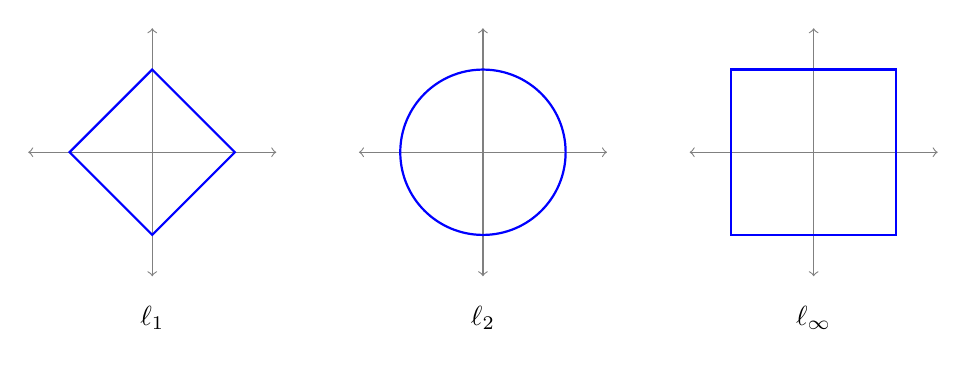
\begin{tikzpicture}[scale=1.05]
    \begin{scope}[shift={(0,0)}]
        \draw[<->, thin, color=gray] (-1.5,0) -- (1.5,0);
        \draw[<->, thin, color=gray] (0,-1.5) -- (0,1.5);
        \draw[thick, color=blue] (1,0) -- (0,1) -- (-1,0) -- (0,-1) -- cycle;
        \node at (0,-2) {$\ell_1$};
    \end{scope}
    \begin{scope}[shift={(4,0)}]
        \draw[<->, thin, color=gray] (-1.5,0) -- (1.5,0);
        \draw[<->, thin, color=gray] (0,-1.5) -- (0,1.5);
        \draw[thick, color=blue] (0,0) circle (1);
        \node at (0,-2) {$\ell_2$};
    \end{scope}
    \begin{scope}[shift={(8,0)}]
        \draw[<->, thin, color=gray] (-1.5,0) -- (1.5,0);
        \draw[<->, thin, color=gray] (0,-1.5) -- (0,1.5);
        \draw[thick, color=blue] (1,1) -- (-1,1) -- (-1,-1) -- (1,-1) -- cycle;
        \node at (0,-2) {$\ell_\infty$};
    \end{scope}
\end{tikzpicture}
\end{center}

In particular, distances measured in these metrics differ, but not by much -- each of these unit circles can be sandwiched between scaled copies of the others. We will return to this observation when we discuss \emph{equivalence} of metrics.

\begin{example}[Uniform Metric]
    Let $S$ be a set, and let $\ell_{\infty}(S)$ be the set of all bounded scalar functions on $S$. We define the $\ell_{\infty}$-norm of $f \in \ell_{\infty}(S)$ by
    $$
    \norm{f} = \norm{f}_{\infty} = \sup_{x \in S}|f(x)|,
    $$
    also called the $\sup$ norm or the uniform norm. From this we can define $d(f, g) = \norm{f - g}_{\infty}$ called the \vocab{uniform metric} on $\ell_{\infty}(S)$.
\end{example}

\begin{example}[$L_p$-Norm]
    Let $\mathcal{C}[a, b]$ be the set of all continuous functions defined on the closed and bounded interval $[a, b]$. Then for $p \geq 1$ we can define the \vocab{$L_p$-norm} of $f \in \mathcal{C}[a, b]$ by
    $$
    \norm{f}_p = \left(\int_a^b |f(x)|^p \dd x\right)^{1/p}.
    $$
    This defines\footnote{If you want to check that $d_p$ satisfies the metric space axioms, you do need the \emph{Minkowski inequality}, which we will not discuss.} the \vocab{$L_p$-metric}, $d_p(f, g) = \norm{f - g}_{p}$.
\end{example}

\begin{example}[Discrete Metric]
Let $M$ be any set. Then
$$
d(x, y) = \begin{cases}
    0 &\mbox{if } x = y, \\
    1 &\mbox{if } x \neq y.
   \end{cases}
$$
defines the metric called the \vocab{discrete metric}, and $(M, d)$ is called a \vocab{discrete metric space}.
\end{example}

\begin{example}[Word Metric]
    Let $G$ be a group generated by $S \subset G$, where $e \not \in S$ and $x \in S$ implies $x^{-1} \in S$. Then
    $$
    d(x, y) = \min \{n \geq 0 \mid \text{there exists } s_1, \dots, s_n \in S \text{ such that } y = x s_1 \cdots s_n \}
    $$
    defines the \vocab{word metric}.
\end{example}

\begin{example}[$p$-adic Metric]
    Fix a prime $p \in \N$. We define
    $$
    d(x, y) = \begin{cases}
        0 &\mbox{if } x = y, \\
        p^{-n} &\mbox{if } x \neq y \text{ where } x - y = p^n m \text{ with } p \nmid m.
       \end{cases}
    $$
    defines a metric on $\Z$ called the \vocab{$p$-adic metric}.
\end{example}

\subsection{Subspaces}

As with many mathematical objects, it can be useful to discuss the substructure to a metric space.

\begin{definition}[Subspace]
    Let $(M, d)$ be a metric space and let $N \subset M$. Then $d$ is a metric on $N$, and $(N, d)$ is a \vocab{subspace} of $M$.    
\end{definition}

\begin{example}[$\Q$ is a subspace of $\R$]
$\Q$ with the metric $d(x, y) = |x - y|$ is a subspace of $\R$.   
\end{example}

\begin{example}[$\mathcal{C}{[a, b]}$ is a subspace of $\ell_{\infty}({[a, b]})$]
    Since every continuous function on a closed, bounded interval is bounded, it follows that $\mathcal{C}[a, b]$ is a subset of $\ell_{\infty}([a, b])$, so $\mathcal{C}[a, b]$ with the uniform metric is a subspace of $\ell_{\infty}([a, b])$.
\end{example}

Given two metric spaces, there is a number of natural construction of another metric space which has those two metric spaces as subspaces.

\begin{definition}[Product Space]    
    Let $(M, d)$ and $(M', d')$ be metric spaces. Then each of the following defines a metric on $M \times M'$:
    \begin{align*}
        d_1((x, x'), (y, y')) &= d(x, y) + d'(x', y') ,\\
        d_2((x, x'), (y, y')) &= \left(d(x, y)^2 + d'(x', y')^2\right)^{1/2} ,\\
        d_{\infty}((x, x'), (y, y')) &= \max\{d(x, y), d'(x', y')\}.
    \end{align*}
    We denote the metric space $(M \times M', d_p)$ by $M \oplus_p M'$.
\end{definition}

\begin{remark}
    There is no canonical choice of which of $\{d_1, d_2, d_{\infty}\}$ we take as the product metric. Indeed, it's straightforward to show that
    $$
    d_{\infty} \leq d_2 \leq d_1 \leq 2 d_{\infty},
    $$
    and later on when we discuss concepts such as convergence we will see that because of this fact, the exact choice of metric doesn't matter \emph{that} much.
\end{remark}

Of course, this construction extends naturally to any finite number of metric spaces.

\subsection{Convergence}

Metric spaces give us a measure of closeness, and we know that in $\R$ and $\C$ that convergence is really just a notion of a sequence getting close to some `limiting value'. Indeed, convergence as we defined it before directly translates into the language of metric spaces.

\begin{definition}[Convergence]
    Let $(M, d)$ be a metric space. A sequence $a_1, a_2, \dots \in M$ is said to \vocab{converge} to the limit $a \in M$ if given any $\varepsilon > 0$, we can find an integer $N$ such that $d(a_n, a) < \varepsilon$ for all $n \geq N$. We write $a_n \rightarrow a$ as $n \rightarrow \infty$.
\end{definition}

A straightforward but useful thing to note is that this definition implies $a_n \rightarrow a$ if and only if $d(a_n, a) \rightarrow 0$ in $\R$.

Now we need to go back to all of the theorems about convergence that were proved in an earlier Analysis course and check if they still hold for a general Metric space (that is, if they don't really use the structure of $\R$, apart from closeness).

\begin{lemma}[Uniqueness of Limits]
    If $a_n \rightarrow a$ and $a_n \rightarrow b$ in a metric space $M$, then $a = b$.
\end{lemma}
\begin{proof}
	Assume that $a \neq b$. Given any $\epsilon > 0$, we can find integers $N_1$ and $N_2$ such that
	\begin{align*}
		d(a_n, a) \leq \epsilon, \quad \text{ for all $n \geq N_1$}\\
		d(a_n, b) \leq \epsilon, \quad \text{ for all $n \geq N_2$}
	\end{align*}
	Then letting $\epsilon = d(a, b)/3$ and taking $N = \max\{N_1, N_2\}$, we have by the triangle inequality
	$$
	d(a, b) \leq d(a, a_n) + d(a_n, b) \leq 2\epsilon = \frac{2}{3} d(a, b)
	$$
	for all $n \geq N$.
	Thus we must have $d(a, b) = 0$, and $a = b$, contradicting our assumption.
\end{proof}

\begin{lemma}[Convergence of Subsequences]
    If $a_n \rightarrow a$ as $n \rightarrow \infty$ in a metric space $M$, and $n(1) < n(2) < \cdots$, then $a_{n(j)} \rightarrow a$ as $j \rightarrow \infty$.
\end{lemma}
\begin{proof}[Proof Sketch]
    Take the old proof from $\R$ and $\C$ and replace the absolute values with the metric!
\end{proof}

\subsection{Continuity}

As with convergence, we also get a direct generalization of the notion of continuity.

\begin{definition}[Continuity]
    Let $f: M \rightarrow M'$ be a function between metric spaces $(M, d)$ and $(M', d')$. Then for $a \in M$, we say that $f$ is \vocab{continuous} at $a$ if given any $\varepsilon > 0$ we can find a $\delta > 0$ such that $d'(f(x), f(a)) < \varepsilon$ for all $x \in M$ such that $d(x, a) < \delta$.

    We say that $f$ is \vocab{continuous} if $f$ is continuous at $a$ for all $a \in M$.
\end{definition}

\begin{proposition}[Sequence Definition of Continuity]
    Let $f: M \rightarrow M'$ be a function between metric spaces, and let $a \in M$. 
    Then $f$ is continuous at $a$ if and only if $x_n \rightarrow a$ in $M$ implies that $f(x_n) \rightarrow f(a)$ in $M'$.
\end{proposition}

We also keep the same standard properties of continuity as before.

\begin{proposition}[Sums, Products, and Reciprocals of Continuous Functions]
	Let $f, g: M \rightarrow \R$ be scalar functions on a metric space $M$. Then the following hold.
	\begin{enumerate}[label=(\roman*)]
		\item If $f$ and $g$ are continuous at $a$, then so is their sum $f + g$.
		\item If $f$ and $g$ are continuous at $a$, then so is their product $fg$.
		\item If $N = \{x \in M \mid g(x)\neq 0\}$, then if $f$ and $g$ are continuous at $a \in N$, then so is $f/g$.
	\end{enumerate}
\end{proposition}

\begin{proposition}[The Composition of Continuous Functions is Continuous]
	Let $f: M \rightarrow M'$ and $g: M' \rightarrow M''$ with $M, M', M''$ all metric spaces. Then if $f$ is continuous at $a \in M$ and $g$ is continuous at $f(a)$, then $g \circ f$ is also continuous at $a$.
\end{proposition}

\begin{example}[Constant Function]
    Consider the constant function $f: M \rightarrow M'$ with $f(x) = b$ for some $b \in M'$. Then $f$ is continuous.
\end{example}

\begin{example}[Identity Function]
    Consider the identity function $\operatorname{id}: M \rightarrow M$. This is continuous at all $a \in M$, as given $\varepsilon > 0$ we can take $\delta = \varepsilon$, and if $d(x, a) < \delta$ then $d(\operatorname{id}(x), \operatorname{id}(a)) = d(x, a) < \delta = \varepsilon$.
\end{example}

\begin{example}[Polynomials]
    Using the examples above, we get that polynomials are always continuous.
\end{example}

\begin{example}[Metrics are Continuous]
    Let $(M, d)$ be a metric space. Then $d$ is a function between metric spaces, $d: M \oplus_p M \rightarrow \R$ (where we take some $p \in \{1, 2, \infty\}$).

    Given $v = (x, x')$ and $w = (y, y') \in M \oplus_p M$, then
    $$|d(v) - d(w)| = |d(x, x') - d(y, y')| \leq d(x, y) + d(x', y') = d_1(v, w) \leq 2d_p(v, w).$$
    So $\delta = \varepsilon/2$ will do.
\end{example}

\begin{definition}[Isometric and Lipschitz]
    Let $f: M \rightarrow M'$ be a function between metric spaces. Then $f$ is \vocab{isometric} if for all $x, y \in M$ we have $d'(f(x), f(y)) = d(x, y)$.

    We say that $f$ is \vocab{Lipschitz} if there exists some $c \in \R^+$ such that $d'(f(x), f(y)) \leq cd(x, y)$.
\end{definition}

\begin{definition}[Uniform Continuity]
    Let $f: M \rightarrow M'$ be a function between metric spaces. We say that $f$ is \vocab{uniformly continuous} if given $\varepsilon > 0$, there exists some $\delta > 0$ such that for all $x, y \in M$ with $d(x, y) < \delta$ we have $d'(f(x), f(y)) < \varepsilon$. 
\end{definition}

We can easily see that $f$ isometric implies that it's Lipschitz, and $f$ Lipschitz implies that it's uniformly continuous. Also, if $f$ is isometric then it must be injective (but not necessarily surjective). If $f$ is also surjective then we call it a \vocab{isometry}.

If there exists an isometry between two metric spaces $M$ and $M'$, we say that they are \vocab{isometric}.

\begin{example}
    Let $(M,d)$ and $(M', d')$ be metric spaces, and fix some $y \in M'$. Then if we define $f: M \rightarrow M \oplus_p M'$ by $f(x) = (x, y)$, we have $d_p(f(x), f(z)) = d_p((x, y), (x, z)) = d(x, z)$. So $f$ is an isometry, and $M \times \{y\}$ is an isometric copy of $M$ in the space $M \oplus_p M'$. 
\end{example}

\subsection{The Topology of a Metric Space}

While we will discuss topology and topological spaces later, it's worth looking at a few of the core ideas in the context of metric spaces.

It seems that there are some concepts in metric spaces that don't \emph{really} rely on the metric, just about the closeness of points. The point of this section is looking to see exactly what type of relations are these, so that we can generalize them to a setting where we don't use a metric.

We begin with the familiar concept of an open ball.

\begin{definition}[Open Ball]
    Let $M$ be a metric space, $x \in M$ and $r > 0$. The \vocab{open ball} in $M$ of center $x$ and radius $r$ is the set $D_r(x)$ given by
    $$
    D_r(x) = \{y \in M \mid d(x, y) < r \}.
    $$
\end{definition}

The idea of open balls is a natural one, and it even fits naturally into some of our previous definitions.

For example, we say that $x_n \rightarrow x$ in $M$ if and only if for all $\varepsilon > 0$, there is some positive integer $N$ such that $n \geq N$ implies that $x_n \in D_{\varepsilon}(x)$.

Similarly, for a function $f: M \rightarrow M'$ we say that $f$ is continuous at $x \in M$ if and only if for all $\varepsilon > 0$ there exists some $\delta > 0$ such that $f(D_{\delta}(x)) \subset D_{\varepsilon}(f(x))$.

\begin{definition}[Closed Ball]
    Let $M$ be a metric space, $x \in M$ and $r > 0$. The \vocab{closed ball} in $M$ of center $x$ and radius $r$ is the set $B_r(x)$ given by
    $$
B_r(x) = \{y \in M \mid d(x, y) \leq r\}.
    $$
\end{definition}

\begin{example}[Open and Closed Ball in $\R$]
    In $\R$, we have $D_r(x) = (x - r, x + r)$, and $B_r(x) = [x - r, x + r]$.
\end{example}

We now move to define some concepts that will be a little less straightforward, but should come together later on as we discuss more topology.

\begin{definition}[Neighborhood]
    Let $M$ be a metric space, and let $U \subset M$. For $x \in M$, we say that $U$ is a \vocab{neighborhood} of $x$ in $M$ if there exists some $r > 0$ such that $D_r(x) \subset U$.
\end{definition}
\begin{definition}[Open]
    We say that $U$ is \vocab{open} in $M$ if for all $x$ in $U$ there is some $r > 0$ such that $D_r(x) \subset U$. That is, if $U$ is a neighborhood for all of its points.
\end{definition}

\begin{example}[Upper Half of the Complex Plane is Not Open]
    Consider the set $H = \{z \in \C \mid \im z \geq 0 \}$.
    Then let $w \in H$, and let $\delta = \im w$. If $\delta > 0$, then $D_{\delta}(w) \subset H$, and if $\delta = 0$, then for all $r > 0$ $D_r(w) \not \subset H$. Thus $H$ is not open.
\end{example}

We commonly use the seeming tautological fact that open balls are open.

\begin{lemma}
    Open balls are open.
\end{lemma}
\begin{proof}
    Consider some open ball $D_r(x)$ in a metric space $M$. Then let $y \in D_r(x)$, and set $\delta = r - d(x, y)$. Then $\delta >0$, and if $z \in D_{\delta}(y)$ then
    $$
    d(z, x) \leq d(z, y) + d(y, x) < \delta + d(x, y) = r,
    $$
    so $z \in D_r(x)$. This shows that $D_{\delta}(y) \subset D_r(x)$.
\end{proof}

\begin{corollary}
    Let $M$ be a metric space, $U \subset M$ and $x \in M$. Then $U$ is a neighborhood of $x$ if and only if there exists an open subset $V$ of $M$ such that $x \in V \subset U$.
\end{corollary}
\begin{proof}[Proof Sketch]
    Check definitions.
\end{proof}

This notion of neighborhoods and open sets is sufficient to describe both convergence and continuity in a metric space on its own.

\begin{proposition}[Convergence using Open Sets \& Neighborhoods]
    In a metric space $M$, the following are equivalent.
    \begin{enumerate}[label=(\roman*)]
        \item $x_n \rightarrow x$;
        \item For all neighborhoods $U$ of $x$ in $M$, there exists some positive integer $N$ such that $n \geq N$ implies $x_n \in U$;
        \item For all open subsets $U$ of $M$ with $x \in U$, there is a positive integer $N$ such that for all $n \geq N$ we have $x_n \in U$.
    \end{enumerate}
\end{proposition}
\begin{proof}
    \emph{(i) implies (ii)}. Let $U$ be a neighborhood of $x$ in $M$. Then by definition there exists some $\varepsilon > 0$ such that $D_{\varepsilon}(x) \subset U$. Then since $x_n \rightarrow x$, there's an $N \in \N$ such that $n \geq N$ implies $d(x_n, x) < \varepsilon$, that is, $x_n \in D_{\varepsilon}(x)$.

    \emph{(ii) implies (iii)}. This is clear since any open set $U$ with $x \in U$ is a neighborhood of $x$.

    \emph{(iii) implies (i)}. Given some $\varepsilon > 0$, $U = D_{\varepsilon}(x)$ is open and $x \in U$. Then by (iii) there's an $N \in \N$ such that $n \geq N$ implies $x_n \in U$, that is, $d(x_n, x) < \varepsilon$.
\end{proof}

\begin{proposition}[Local Continuity using Open Sets \& Neighborhoods]
    Let $f: M \rightarrow M'$ be a function between metric spaces, and let $x \in M$. Then the following are equivalent:
    \begin{enumerate}[label=(\roman*)]
        \item $f$ is continuous at $x$;
        \item For all neighborhoods $V$ of $f(x)$ in $M'$, there exists a neighborhood $U$ of $x$ in $M$ such that $f(U) \subset V$;
        \item For all neighborhoods $V$ of $f(x)$ in $M'$, $f^{-1}(V)$ is a neighborhood of $x$ in $M$.
    \end{enumerate}
\end{proposition}
\begin{proof}
    \emph{(i) implies (ii)}. Let $V$ be a neighborhood of $f(x)$ in $M'$. Then by definition there exists some $\varepsilon > 0$ such that $D_{\varepsilon}(f(x)) \subset V$. Since $f$ is continuous at $x$, there exists $\delta > 0$ such that $f(D_{\delta}(x)) \subset D_\varepsilon(f(x))$. Then $U = D_{\delta}(x)$ is a neighborhood of $x$ in $M$, and $f(U) \subset V$.

    \emph{(ii) implies (iii)}. Let $V$ be a neighborhood of $f(x)$ in $M'$. Then by (ii) there is a neighborhood $U$ of $x$ in $M$ such that $f(U) \subset V$. Then $U \subset f^{-1}(V)$, and since $U$ is a neighborhood of $x$ in $M$, there is some $r > 0$ with $D_r(x) \subset U \subset f^{-1}(V)$. Thus $f^{-1}(V)$ is a neighborhood of $x$ in $M$.

    \emph{(iii) implies (i)}.
    Given $\varepsilon > 0$, $V = D_{\varepsilon}(f(x))$ is a neighborhood of $f(x)$ in $M'$. By (iii), $f^{-1}(V)$ is a neighborhood of $x$ in $M$. So there exists $\delta > 0$ with $D_{\delta}(x) \subset f^{-1}(V)$. Then $f(D_{\delta}(x)) \subset V = D_{\varepsilon}(f(x))$.
\end{proof}

\begin{proposition}[Global Continuity using Open Sets \& Neighborhoods]
    Let $f: M \rightarrow M'$ be a function between metric spaces. Then the following are equivalent:
    \begin{enumerate}[label=(\roman*)]
        \item $f$ is continuous;
        \item $f^{-1}(V)$ is open in $M$ for all open subsets $V$ of $M'$.
    \end{enumerate}
\end{proposition}
\begin{proof}
    \emph{(i) implies (ii)}. Let $V$ be open in $M'$. Let $x \in f^{-1}(V)$. Then $f(x) \in V$. Since $V$ is open, there's some $\varepsilon > 0$ such that $D_{\varepsilon}(f(x)) \subset V$. Since $f$ is continuous at $x$, there's a $\delta > 0$ such that $f(D_{\delta}(x)) \subset D_{\varepsilon}(f(x))$. Therefore $D_{\delta}(x) \subset f^{-1}(D_\varepsilon (f(x))) \subset f^{-1}(V)$. Thus $f^{-1}(V)$ is open in $M$.

    \emph{(ii) implies (i)}. Let $x \in M$, and let $\varepsilon > 0$. Then $V = D_{\varepsilon}(f(x))$ is open in $M'$. By (ii) $f^{-1}(V)$ is open in $M$, also $x \in f^{-1}(V)$ and $f(x) \in V$. Then by definition there's a $\delta > 0$ such that $D_{\delta}(x) \subset f^{-1}(V)$, so $f(D_{\delta}(x)) \subset V = D_\varepsilon(f(x))$.
\end{proof}

We can now write down what the \emph{topology} of a metric space is. We are going to study topology in general later on, but we can use some properties that occur here to inform how we define things more generally afterwards.

\begin{definition}[Topology of a Metric Space]
    The \vocab{topology} of a metric space $M$ is the family of all open subsets of $M$.
\end{definition}

\begin{proposition}[Basic Properties]
    The topology of a metric space satisfies the following.
    \begin{enumerate}[label=(\roman*)]
        \item $\emptyset$ and $M$ are open.
        \item If $U_i$ is open in $M$ for all $i$ in some index set $I$, then $\bigcup_{i \in I} U_i$ is open in $M$.
        \item $U, V$ open in $M$ implies $U \cap V$ open in $M$.
    \end{enumerate}
\end{proposition}
\begin{proof}
    \emph{Part (i)}. This is clear.

    \emph{Part (ii)}. Given $x \in \bigcup_{i \in I} U_i$, then there's some $i_0 \in I$ with $x \in U_{i_0}$. Then $U_{i_0}$ is open, so by definition there's an $r > 0$ with $D_r(x) \subset U_{i_0} \subset \bigcup_{i \in I} U_i$.

    \emph{Part (iii)}. Given $x \in U \cap V$, since $U$ is open and $x \in U$, there's an $r > 0$ with $D_r(x) \subset U$, and since $V$ is open and $x \in V$, there's an $s > 0$ with $D_s(x) \subset V$. Then letting $t = \min\{r, s\}$, we have $t >0$ and $D_t(x) = D_r(x) \cap D_s(x) \subset U \cap V$.
\end{proof}

\begin{definition}[Closed]
    A subset $A$ of a metric space $M$ is \vocab{closed} in $M$ if for every sequence $x_n \in A$ that is convergent in $M$, we have $\lim_{n \to \infty} x_n \in A$.
\end{definition}

\begin{lemma}
    Closed balls are closed.
\end{lemma}
\begin{proof}
    Consider $B_r(x) = \{y \in M \mid d(y, x) \leq r\}$ in a metric space $M$, and a sequence $x_n \in B_r(x)$ such that $x_n \rightarrow z$. We need to show that $z \in B_r(x)$. We have
    \begin{align*}
        d(z, x) &\leq d(z, x_n) + d(x_n, x) \\
            &\leq d(z, x_n) + r \rightarrow r
    \end{align*}
    as $n \rightarrow \infty$. Thus $d(z, x) \leq r$, and hence $z \in B_r(x)$.
\end{proof}

\begin{example}[Closed but Not Open, and Open but Not Closed Sets]
    The set $[0, 1] = B_{\frac{1}{2}}(1/2)$ is closed in $\R$. $[0, 1]$ is not open, for example $D_r(0) \not \subset [0, 1]$ for any $r > 0$.

    The set $(0, 1) = D_{\frac{1}{2}}(1/2)$ is open, but it is not closed. Take $1/(n + 1) \in (0, 1)$ for all $n \in \N$. Then $1/(n + 1) \rightarrow 0$ in $\R$ but $0 \not \in (0, 1)$.
\end{example}

\begin{example}[An Open and Closed Set]
   $\R$ is open and closed in $\R$.
\end{example}

\begin{example}[A Neither Open or Closed Set]
    The set $(0, 1]$ in $\R$ is neither open nor closed.
\end{example}

\begin{lemma}[Relating Closed and Open]
    Let $A$ be a subset of a metric space $M$. Then $A$ is closed in $M$ if and only if $M \backslash A$ is open in $M$.
\end{lemma}
\begin{proof}
    Assume $A$ is closed, and that $M \backslash A$ is not open. Then there exists $x \in M \backslash A$ such that for all $r > 0$ we have $D_r(x) \not \subset M\backslash A$. 
    Hence for all $n$ there exists $x_n \in D_{1/n}(x) \cap A$. Then $d(x_n, x) < 1/n \rightarrow 0$, so $x_n \rightarrow x$ in $M$ and $x_n \in A$ for all $n$, which contradicts that $A$ is closed.

    Now suppose that $M \backslash A$ is open but $A$ is not closed. Then there exists some sequence $x_n$ in $A$ such that $x_n \rightarrow x$ in $M$ but $x \not \in A$. Since $x \in M \backslash A$ and $M \backslash A$ is open, there exists $\varepsilon > 0$ with $D_\varepsilon(x) \subset M \backslash A$. Then since $x_n \rightarrow x$, there is some $N \in \N$ such that for all $n \geq N$ we have $x_n \in D_{\varepsilon}(x)$, and hence $x_n \in M \backslash A$, which is a contradiction.
\end{proof}

We previously met isometries, which were maps between metric spaces that preserved the distance function. Now that we are trying to look slightly away from metrics and more towards open sets and neighborhoods, it's natural to think of a new definition of a function between metric spaces that preserves open sets.

\begin{definition}[Homeomorphism]
    A map $f: M \rightarrow M'$ between metric spaces is a \vocab{homeomorphism} if $f$ is a bijection, and $f$ and $f^{-1}$ are both continuous.

    Equivalently, $f$ is a homeomorphism if for all open sets $V$ in $M'$, $f^{-1}(V)$ is open in $M$, and for all open sets $U$ in $M$, $f(U)$ is open in $M'$.

    If there is a homeomorphism between $M$ and $M'$, we say that $M$ and $M'$ are \vocab{homeomorphic}.
\end{definition}

\begin{example}
    The metric spaces $(0, \infty)$ and $(0, 1)$ are homeomorphic, with the homeomorphism $x \mapsto 1/(x + 1)$ and inverse $x \mapsto 1/x - 1$.
\end{example}

While it is true that every isometry is a homeomorphism, the converse is absolutely false.

We will say that two metrics on a set are equivalent if they induce the same topology.

\begin{definition}[Equivalent Metrics]
    Let $d$ and $d'$ be metrics on a set $M$. We say that $d$ and $d'$ are \vocab{equivalent}, denoted $d \sim d'$, if they define the same topology on $M$. That is, for $U \subset M$, $U$ is open in $(M, d)$ if and only if $U$ is open in $(M, d')$.
\end{definition}

So $d \sim d'$ if and only if $\operatorname{id}: (M, d) \rightarrow (M, d')$ is a homeomorphism. 

Note that if $d \sim d'$, then $(M, d)$ and $(M, d')$ have the same convergent sequences and the same continuous maps.

\begin{definition}[Uniformly and Lipschitz Equivalent]
    Let $d$ and $d'$ be metrics on a set $M$. We say that $d$ and $d'$ are \vocab{uniformly equivalent} if $\operatorname{id}: (M, d) \rightarrow (M, d')$ and $\operatorname{id}: (M, d') \rightarrow (M, d)$ are uniformly continuous, and write $d \sim_u d'$.

    We will say $d$ and $d'$ are \vocab{Lipschitz equivalent} if these functions are Lipschitz, and write $d \sim_{Lip} d'$.
\end{definition}

Note that $d \sim_{Lip} d'$ if and only if there exists $a > 0$ and $b > 0$ such that
$$
a d(x, y) \leq d'(x, y) \leq b d(x, y),
$$
and also note that $d \sim_{Lip} d'$ implies $d \sim_u d'$ implies $d \sim d'$.

\begin{example}
    Given a metric space $(M, d)$, $d'(x, y) = \min\{1, d(x, y)\}$ defines a metric on $M$, and $d' \sim_u d$.
\end{example}

\begin{example}
    On a product space $M \times M'$, the metrics $d_1$, $d_2$ and $d_{\infty}$ are pairwise Lipschitz equivalent.
\end{example}

\begin{example}
    On $C[0, 1]$, the $L_1$-metric and the uniform metric are \emph{not} equivalent.
\end{example}

We will return to these topological ideas later on.

\section{Completeness and the Contraction Mapping Theorem}

\subsection{Completeness}

In $\R$ and $\C$, every Cauchy sequence is convergent. In what other spaces is this true?

\begin{definition}[Cauchy Sequence]
    A sequence $x_n$ in a metric space $M$ is \vocab{Cauchy} if given $\varepsilon > 0$, there's some positive integer $N$ such that $n, m \geq N$ implies that $d(x_n, x_m) < \varepsilon$.
\end{definition}

\begin{definition}[Bounded]
    A sequence $x_n$ in a metric space $M$ is \vocab{bounded} if there exists some $z \in M$ and $r > 0$ such that for all $n$ we have $x_n \in B_r(z)$.
\end{definition}

\begin{lemma}[Convergent Implies Cauchy Implies Bounded]
    Every convergent sequence is Cauchy, and every Cauchy sequence is bounded.
\end{lemma}
\begin{proof}
    Let $x_n$ be a sequence in metric space $M$. 
    
    Suppose $x_n$ is convergent in $M$, and let $x = \lim_{n \to \infty} x_n$.
    Given $\varepsilon > 0$, there is some positive integer $N$ such that $n \geq N$ implies $d(x_n, x) < \varepsilon/2$.
    Then for all $m, n \geq N$, $d(x_m, x_n) \leq d(x_m, x) + d(x, x_n) < \varepsilon$. Thus if a sequence converges, then it's Cauchy.

    Now assume that $x_n$ is Cauchy in $M$. Then there's a positive integer $N$ such that for all $m, n \geq N$ we have $d(x_m, x_n) < 1$. In particular, $d(x_n, x_N) < 1$ for $n \geq N$, that is, $x_n \in B_1(x_N)$ for $n \geq N$.
    So let $r = \max\{d(x_1, x_N), \dots, d(x_{N - 1}, x_N), 1\}$. Then $x_n \in B_r(x_N)$ for all $n \in \N$, and so $x_n$ is bounded.
\end{proof}

In general, being bounded does not imply that a sequence is Cauchy (for example, take the sequence $0, 1, 0, 1, \dots$).

Slightly more subtle is that being Cauchy doesn't imply convergence, and we can construct a somewhat silly example. For example, $x_n = 1/n$ is Cauchy but doesn't converge in the metric space $(0, \infty)$.
It seems that this example works because there's something `missing' from the metric space -- the limit of a sequence. Indeed, in this section we will care about metric spaces where such an implication \emph{does hold}, in `complete' metric spaces.

\begin{definition}[Completeness]
    A metric space $M$ is \vocab{complete} if every Cauchy sequence in $M$ converges in $M$.
\end{definition}

\begin{example}
    $\R$ and $\C$ are complete.
\end{example}

\begin{proposition}
    If $M$ and $M'$ are complete metric spaces, then so is $M \oplus_p M'$.
\end{proposition}
\begin{proof}
    Let $z_n = (x_n, x_n')$ be a Cauchy sequence in $M \oplus_p M'$. Since $d(x_m, x_n) \leq d_p(z_m, z_n)$ and $d'(x_m', x_n') \leq d_p(z_m, z_n)$, both $x_n$ and $x_n'$ are Cauchy in $M$ and $M'$ respectively. By completeness, $x_n \rightarrow x$ in $M$ and $x_n' \rightarrow x'$ in $M'$, and then letting $z = (x, x')$ we have
    $$
    d_p(z_n, z) \leq d_1(z_n, z) = d(x_n, x) + d'(x_n', x') \rightarrow 0,
    $$
    so $z_n \rightarrow z$ in $M \oplus_p M'$.
\end{proof}

\begin{example}
    $\R^n$ and $\C^n$ are complete in the $\ell_p$-metric.
\end{example}


\begin{theorem}[Completeness of a Function Space]
    Let $S$ be any set. Then $\ell_{\infty}(S)$ is complete in the uniform metric $D$.
\end{theorem}
\begin{proof}
    Let $f_n$ be a Cauchy sequence in $\ell_{\infty}(S)$. Then given $\varepsilon> 0$, there is some positive integer $N$ such that for all $n, m \geq N$ we have
    $$
    D(f_m, f_n) = \sup_{x \in S} |f_m(x) - f_n(x)| < \varepsilon.
    $$
    So $f_n$ is uniformly Cauchy. By the general principle of uniform convergence, $f_n$ converges uniformly to some function $f$ on $S$.
    We also know that $f$ is bounded, so $f \in \ell_{\infty}(S)$. 
    Now given $\varepsilon > 0$, there's some $N \in \N$ such that for all $n \geq N$ and $x \in S$ we have
    $$
    |f_n(x) - f(x)| < \varepsilon,
    $$
    and thus for $n \geq N$ we have $\sup_{x \in S} |f_n(x) - f(x)| = D(f_n, f) \leq \varepsilon$, so $f_n \rightarrow f$ in $(\ell_{\infty}(S), D)$.
\end{proof}

\begin{proposition}[Completeness of a Subspace]
    Let $N$ be a subspace of a metric space $M$. 
    \begin{enumerate}[label=(\roman*)]
        \item If $N$ is complete, then $N$ is closed in $M$.
        \item If $M$ is complete and $N$ is closed in $M$, then $N$ is complete.
    \end{enumerate}
\end{proposition}
\begin{proof}
    \emph{Part (i)}. Let $x_n$ be a sequence in $N$ and assume that $x_n \rightarrow x$ in $M$. We then need $x \in N$. Since $x_n$ is convergent in $M$, $x_n$ must also be Cauchy in $M$, and thus it is Cauchy in $N$. Then since $N$ is complete, we must have $x_n \rightarrow y \in N$. But then $x_n \rightarrow y \in M$, and by uniqueness of limits, $y = x$ and $x \in N$.

    \emph{Part (ii)}. Let $x_n$ be a Cauchy sequence in $N$. Then $x_n$ is Cauchy in $M$. Since $M$ is complete, $x_n \rightarrow x$ in $M$ for some $x \in M$. Since $N$ is closed in $M$, we have $x \in N$. So $x_n \rightarrow x$ in $N$.
\end{proof}

\begin{theorem}
    Let $(M, d)$ be a metric space, and define
    $$
    C_b(M) = \{f \in \ell_{\infty}(M) \mid f \text{ is continuous} \}.
    $$
    This is a subspace of $\ell_{\infty}(M)$ in the uniform metric $D$.

    Then $C_b(M)$ is complete in the uniform metric.
\end{theorem}
\begin{proof}
It suffices to show that $C_b(M)$ is closed in $\ell_{\infty}(M)$. Let $f_n$ be a sequence in $C_b(M)$, and assume that $f_n \rightarrow f$ in $\ell_{\infty}(M)$. We need to show that $f$ is continuous.

Given some $a \in M$ and $\varepsilon > 0$, since $f_n \rightarrow f$ in $\ell_{\infty}(M)$, we can fix an $n \in \N$ such that $D(f_n, f) < \varepsilon$.
Since $f_n$ is continuous at $a$, there's a $\delta > 0$ such that for all $x \in M$ we have $d(x, a) < \delta$ implying $|f_n(x) - f_n(a)| < \varepsilon$. Hence for all $x \in M$ if $d(x,a) < \delta$ then
\begin{align*}
    |f(x) - f(a)| &\leq |f(x) - f_n(x)| + |f_n(x) - f_n(a)| + |f_n(a) - f(a)|  \\
    &\leq 2D(f_n, f) + |f_n(x) - f_n(a)|  \\
    & \leq 3\varepsilon.
\end{align*}
\end{proof}

\begin{corollary}
    $C[a, b]$, the space of continuous functions on the closed bounded interval $[a, b]$ is complete in the uniform metric.
\end{corollary}

This last corollary is going to be surprisingly useful. Completeness of function spaces is what will let us \emph{construct} functions as limits -- and in particular, it is the key to proving the existence of solutions to differential equations, as we are about to see.

\subsection{The Contraction Mapping Theorem}

We now come to the highlight of this section, which is a genuinely useful theorem about complete metric spaces. It concerns \emph{fixed points} of certain well-behaved maps from a metric space to itself.

\begin{definition}[Contraction]
    Let $(M, d)$ be a metric space. A map $f : M \rightarrow M$ is a \vocab{contraction} if there exists some $\lambda$ with $0 \leq \lambda < 1$ such that
    $$
    d(f(x), f(y)) \leq \lambda d(x, y),
    $$
    for all $x, y \in M$.
\end{definition}

That is, a contraction is a map which is Lipschitz with constant strictly less than $1$ -- it shrinks distances by a definite factor. In particular every contraction is (uniformly) continuous.

\begin{theorem}[Contraction Mapping Theorem]\label{thm:contraction}
    Let $M$ be a non-empty complete metric space, and let $f: M \rightarrow M$ be a contraction. Then $f$ has a unique fixed point, that is, there is a unique $z \in M$ such that $f(z) = z$.
\end{theorem}
\begin{proof}
    Let $\lambda \in [0, 1)$ be such that $d(f(x), f(y)) \leq \lambda d(x, y)$ for all $x, y \in M$.

    We first show uniqueness. If $f(z) = z$ and $f(w) = w$, then
    $$
    d(z, w) = d(f(z), f(w)) \leq \lambda d(z, w),
    $$
    and since $\lambda < 1$ this forces $d(z, w) = 0$, so $z = w$.

    Now for existence, the idea is to just pick a point and repeatedly apply $f$, and show that the sequence we get is Cauchy. So fix any $x_0 \in M$ (using non-emptiness), and define the sequence $x_n = f(x_{n - 1})$ for $n \geq 1$. Applying the contraction property repeatedly,
    $$
    d(x_n, x_{n + 1}) = d(f(x_{n-1}), f(x_n)) \leq \lambda d(x_{n - 1}, x_n) \leq \cdots \leq \lambda^n d(x_0, x_1).
    $$
    Then for $m \geq n$, the triangle inequality gives
    $$
    d(x_n, x_m) \leq \sum_{k = n}^{m - 1} d(x_k, x_{k + 1}) \leq \sum_{k = n}^{m - 1} \lambda^k d(x_0, x_1) \leq \frac{\lambda^n}{1 - \lambda} d(x_0, x_1).
    $$
    Since $\lambda^n/(1 - \lambda) \rightarrow 0$ as $n \rightarrow \infty$, given $\varepsilon > 0$ we can find $N$ such that $d(x_n, x_m) < \varepsilon$ for all $m \geq n \geq N$. So the sequence $x_n$ is Cauchy, and since $M$ is complete, $x_n \rightarrow z$ for some $z \in M$.

    Finally, $f$ is continuous, so $x_{n + 1} = f(x_n) \rightarrow f(z)$, but also $x_{n + 1} \rightarrow z$, so by uniqueness of limits $f(z) = z$.
\end{proof}

There is a nice picture of what is going on here for a contraction on $\R$. Starting anywhere and `cobwebbing' between the graph of $f$ and the line $y = x$, the iterates spiral into the fixed point, which is where the graphs cross.

\begin{center}
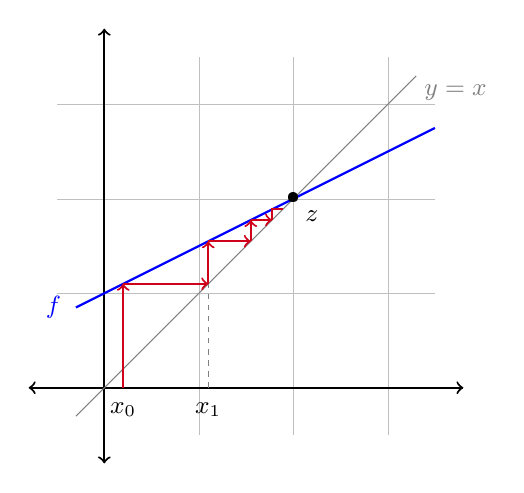
\begin{tikzpicture}[scale=1.2]
    \draw[ultra thin, color=lightgray] (-0.5,-0.5) grid (3.5,3.5);
    \draw[<->] (-0.8,0) -- (3.8,0);
    \draw[<->] (0,-0.8) -- (0,3.8);
    \draw[thin, color=gray] (-0.3,-0.3) -- (3.3,3.3);
    \node[color=gray, anchor=west] at (3.28,3.12) {\small $y = x$};
    \draw[thick, samples=100, smooth, domain=-0.3:3.5, color=blue] plot (\x, {0.5*\x + 1});
    \node[color=blue, anchor=east] at (-0.35,0.85) {\small $f$};
    \draw[color={rgb,255:red,208;green,2;blue,27}, ->] (0.2,0) -- (0.2,1.1);
    \draw[color={rgb,255:red,208;green,2;blue,27}, ->] (0.2,1.1) -- (1.1,1.1);
    \draw[color={rgb,255:red,208;green,2;blue,27}, ->] (1.1,1.1) -- (1.1,1.55);
    \draw[color={rgb,255:red,208;green,2;blue,27}, ->] (1.1,1.55) -- (1.55,1.55);
    \draw[color={rgb,255:red,208;green,2;blue,27}, ->] (1.55,1.55) -- (1.55,1.775);
    \draw[color={rgb,255:red,208;green,2;blue,27}, ->] (1.55,1.775) -- (1.775,1.775);
    \draw[color={rgb,255:red,208;green,2;blue,27}] (1.775,1.775) -- (1.775,1.8875) -- (1.8875,1.8875);
    \node[color=black] at (2,2) {\textbullet};
    \node[color=black, anchor=north west] at (2.02,1.98) {\small $z$};
    \node[anchor=north] at (0.2,-0.05) {\small $x_0$};
    \node[anchor=north] at (1.1,-0.05) {\small $x_1$};
    \draw[ultra thin, color=gray, dash pattern={on 2pt off 2pt}] (1.1,0) -- (1.1,1.1);
\end{tikzpicture}
\end{center}

\begin{remark}
    Letting $m \rightarrow \infty$ in the bound for $d(x_n, x_m)$ in the proof above shows that
    $$
    d(x_n, z) \leq \frac{\lambda^n}{1 - \lambda} d(x_0, x_1),
    $$
    so the iterates converge to the fixed point \emph{exponentially fast}. This makes the contraction mapping theorem practical as a numerical method, not just a theoretical tool.
\end{remark}

Both hypotheses in the theorem -- completeness of the space, and the Lipschitz constant being strictly less than $1$ -- are genuinely needed, as the following examples show.

\begin{example}[Completeness is Necessary]
    Consider $f: \R \backslash \{0\} \rightarrow \R \backslash \{0\}$ given by $f(x) = x/2$. This is a contraction (with $\lambda = 1/2$), but it has no fixed point -- the `missing' fixed point is $0$, and the problem is that $\R \backslash \{0\}$ is not complete.
\end{example}

\begin{example}[Shrinking Distances is Not Enough]
    Consider $f: [1, \infty) \rightarrow [1, \infty)$ given by $f(x) = x + 1/x$. The domain is closed in $\R$ and hence complete, and it's easy to check that $|f(x) - f(y)| < |x - y|$ for all $x \neq y$. But $f$ has no fixed point, since $f(x) - x = 1/x > 0$ everywhere.

    The issue is that there is no single $\lambda < 1$ that works for \emph{all} pairs of points -- the map shrinks distances, but not uniformly so. Similarly, $f(x) = x + 1$ on $\R$ is an isometry ($\lambda = 1$) with no fixed point.
\end{example}

\subsection{Application: Solving Differential Equations}

At first glance, the contraction mapping theorem might look like a curiosity. Its real power comes from applying it to \emph{function spaces}: if we can express `being a solution to a problem' as `being a fixed point of a map on a complete space of functions', then we get existence and uniqueness of solutions in one stroke. The classic application is to differential equations.

Let's warm up with a specific example before proving the general theorem.

\begin{example}[An Unusual Differential Equation]
    Fix $y_0 \in \R$. We will show that there is a unique differentiable function $f: [0, \tfrac{1}{2}] \rightarrow \R$ such that $f(0) = y_0$ and
    $$
    f'(t) = f(t^2) \quad \text{for all } t \in [0, \tfrac{1}{2}].
    $$
    First note that if $f$ is such a solution, then $f$ is differentiable and hence continuous, so $f'(t) = f(t^2)$ is also continuous. Then by the fundamental theorem of calculus,
    $$
    f(t) = y_0 + \int_0^t f(s^2) \dd s.
    $$
    Conversely, if $f \in C[0, \tfrac{1}{2}]$ satisfies this integral equation, then by the fundamental theorem of calculus (the integrand being continuous) $f$ is differentiable with $f'(t) = f(t^2)$, and $f(0) = y_0$. So solving the differential equation is \emph{equivalent} to solving the integral equation in $C[0, \tfrac{1}{2}]$.

    Now let $M = C[0, \tfrac{1}{2}]$ with the uniform metric $D$, which we know is non-empty and complete, and define $T: M \rightarrow M$ by
    $$
    (Tg)(t) = y_0 + \int_0^t g(s^2) \dd s.
    $$
    By the reasoning above, $f$ solves our problem if and only if $Tf = f$. But for $g, h \in M$ and $t \in [0, \tfrac{1}{2}]$,
    $$
    |(Tg)(t) - (Th)(t)| = \left| \int_0^t \left[g(s^2) - h(s^2)\right] \dd s \right| \leq t \sup_{s} |g(s^2) - h(s^2)| \leq \frac{1}{2} D(g, h).
    $$
    Taking the supremum over $t$, we get $D(Tg, Th) \leq \frac{1}{2} D(g, h)$, so $T$ is a contraction. By the contraction mapping theorem, $T$ has a unique fixed point, which is the unique solution to our differential equation.
\end{example}

\begin{remark}
    The choice of the interval $[0, \tfrac{1}{2}]$ mattered only in making the map a contraction -- the same argument gives a unique solution $f_{\delta}$ on $[0, \delta]$ for any $\delta < 1$. By uniqueness, these solutions agree on common domains, so they patch together into a unique solution on $[0, 1)$.
\end{remark}

The same circle of ideas gives the fundamental existence and uniqueness theorem for ordinary differential equations. Before we state it, we need to make sense of integrating a vector-valued function: for continuous $f = (f_1, \dots, f_n): [c, d] \rightarrow \R^n$, we integrate coordinate-wise,
$$
\int_c^d f(t) \dd t = \left( \int_c^d f_1(t) \dd t, \dots, \int_c^d f_n(t)\dd t \right),
$$
and differentiability of such an $f$ also means differentiability of each coordinate, with $f' = (f_1', \dots, f_n')$. A useful fact, which follows from the Cauchy-Schwarz inequality\footnote{Write $v = \int_c^d f(t) \dd t$. Then $\norm{v}^2 = \sum_k v_k \int f_k = \int \langle v, f(t)\rangle \dd t \leq \int \norm{v} \norm{f(t)} \dd t$, and divide by $\norm{v}$.}, is that
$$
\norm{\int_c^d f(t) \dd t} \leq \int_c^d \norm{f(t)} \dd t \leq (d - c)\sup_{t \in [c, d]} \norm{f(t)}.
$$

\begin{theorem}[Picard-Lindel\"of]
    Let $y_0 \in \R^n$, let $a < b$ be reals, $R > 0$, and let
    $$
    \phi: [a, b] \times B_R(y_0) \rightarrow \R^n
    $$
    be a continuous function. Suppose $\phi$ is Lipschitz in the second variable, that is, there is some $K > 0$ such that
    $$
    \norm{\phi(t, x) - \phi(t, y)} \leq K \norm{x - y}
    $$
    for all $t \in [a, b]$ and $x, y \in B_R(y_0)$. Then there exists $\varepsilon > 0$ such that for any $t_0 \in [a, b]$, the initial value problem
    $$
    f'(t) = \phi(t, f(t)), \quad f(t_0) = y_0
    $$
    has a unique solution on $[c, d] = [t_0 - \varepsilon, t_0 + \varepsilon] \cap [a, b]$.
\end{theorem}
\begin{proof}
    Since closed balls are closed, $B_R(y_0)$ is closed and bounded in $\R^n$, and one can check (say, coordinate-wise using Bolzano-Weierstrass, as we did for uniform continuity) that a continuous function on a closed bounded subset of $\R^{n+1}$ is bounded\footnote{We will be able to see this much more cleanly once we have discussed \emph{compactness}.}. So we may set
    $$
    C = \sup\{\norm{\phi(t, x)} \mid t \in [a, b],\ x \in B_R(y_0)\} < \infty,
    $$
    and define $\varepsilon = \min\{R/C, 1/(2K)\}$. Fix $t_0 \in [a, b]$ and let $[c, d] = [t_0 - \varepsilon, t_0 + \varepsilon] \cap [a, b]$.

    As before, we convert the problem into an integral equation. By the fundamental theorem of calculus applied coordinate-wise, a function $f: [c, d] \rightarrow B_R(y_0)$ solves the initial value problem if and only if $f$ is continuous and
    $$
    f(t) = y_0 + \int_{t_0}^t \phi(s, f(s)) \dd s \quad \text{for all } t \in [c, d].
    $$

    Now we set up our function space. Since $B_R(y_0)$ is closed in the complete space $\R^n$, it is complete, and hence the space $M = C([c, d], B_R(y_0))$ of continuous functions $[c, d] \rightarrow B_R(y_0)$ is complete in the uniform metric $D$ (as before, being uniformly Cauchy implies uniform convergence, and the uniform limit of continuous functions into a closed set is continuous into that set). It's also non-empty, as it contains the constant function $t \mapsto y_0$.

    Define $T: M \rightarrow M$ by
    $$
    (Tg)(t) = y_0 + \int_{t_0}^t \phi(s, g(s)) \dd s.
    $$
    We should check this is well defined. If $g \in M$ then $s \mapsto \phi(s, g(s))$ is continuous, so the integral makes sense and $Tg$ is continuous (indeed differentiable). Moreover for $t \in [c, d]$,
    $$
    \norm{(Tg)(t) - y_0} = \norm{\int_{t_0}^t \phi(s, g(s)) \dd s} \leq |t - t_0| \sup_{s \in [c,d]} \norm{\phi(s, g(s))} \leq \varepsilon C \leq R,
    $$
    so $Tg$ does map into $B_R(y_0)$, and $Tg \in M$. By construction, $f$ solves the initial value problem if and only if $Tf = f$.

    Finally, we check that $T$ is a contraction. For $g, h \in M$ and $t \in [c, d]$,
    \begin{align*}
    \norm{(Tg)(t) - (Th)(t)} &= \norm{\int_{t_0}^t \left[\phi(s, g(s)) - \phi(s, h(s))\right] \dd s} \\
    &\leq |t - t_0| \sup_{s \in [c, d]} \norm{\phi(s, g(s)) - \phi(s, h(s))} \\
    &\leq \varepsilon K \sup_{s \in [c, d]} \norm{g(s) - h(s)} \leq \frac{1}{2} D(g, h),
    \end{align*}
    using the Lipschitz hypothesis and $\varepsilon \leq 1/(2K)$. Taking the supremum over $t$ gives $D(Tg, Th) \leq \frac{1}{2}D(g, h)$, so $T$ is a contraction on the non-empty complete metric space $M$, and by the contraction mapping theorem it has a unique fixed point. This fixed point is the unique solution to the initial value problem.
\end{proof}

\begin{remark}
    A few comments on this theorem.
    \begin{enumerate}[label=(\roman*)]
        \item The theorem is \emph{local} -- it only guarantees a solution close to $t_0$. In general there really is no solution on all of $[a, b]$; consider $f' = f^2$, $f(0) = 1$, whose solution $f(t) = 1/(1 - t)$ blows up in finite time.
        \item Any $n$-th order ODE $y^{(n)} = \psi(t, y, y', \dots, y^{(n-1)})$ can be handled by this theorem, by the standard trick of introducing the vector $(y, y', \dots, y^{(n - 1)}) \in \R^n$ and rewriting the equation as a first-order system.
    \end{enumerate}
\end{remark}

\section{Topological Spaces}

When we studied metric spaces, we found that many important concepts -- convergence, continuity, open and closed sets -- could be phrased entirely in terms of \emph{open sets}, with no direct mention of the metric. This suggests a further abstraction: throw away the metric entirely, and take the open sets themselves as the fundamental structure. This is the starting point of \emph{topology}.

\subsection{Topologies}

Recall the basic properties satisfied by the open subsets of a metric space: the empty set and the whole space are open, arbitrary unions of open sets are open, and finite intersections of open sets are open. We take precisely these properties as our axioms.

\begin{definition}[Topology]
    Let $X$ be a set. A \vocab{topology} on $X$ is a family $\tau$ of subsets of $X$ such that
    \begin{enumerate}[label=(\roman*)]
        \item $\emptyset \in \tau$ and $X \in \tau$;
        \item if $U_i \in \tau$ for all $i$ in some index set $I$, then $\bigcup_{i \in I} U_i \in \tau$;
        \item if $U, V \in \tau$, then $U \cap V \in \tau$.
    \end{enumerate}
    A \vocab{topological space} is a pair $(X, \tau)$ where $X$ is a set and $\tau$ is a topology on $X$. The members of $\tau$ are called the \vocab{open sets} of $X$.
\end{definition}

By induction, (iii) implies that any \emph{finite} intersection of open sets is open. As with metric spaces, we usually just refer to `the topological space $X$', leaving the topology implicit.

\begin{example}[Metric Topology]
    Let $(M, d)$ be a metric space. Then the family of all $d$-open subsets of $M$ is a topology on $M$, called the \vocab{metric topology} induced by $d$ -- this is exactly what we proved at the end of our discussion of the topology of metric spaces.
\end{example}

\begin{definition}[Metrizable]
    A topological space $(X, \tau)$ is \vocab{metrizable} if there exists a metric $d$ on $X$ which induces the topology $\tau$.
\end{definition}

Note that equivalent metrics induce the same topology, so a metrizable space never remembers \emph{which} metric it came from. Not every topological space is metrizable, as we shall see shortly. First, some examples of topologies that don't obviously come from metrics.

\begin{example}[Discrete Topology]
    For any set $X$, the family $\tau = \power(X)$ of \emph{all} subsets of $X$ is a topology, called the \vocab{discrete topology}. It is metrizable -- it is induced by the discrete metric, since in that metric $D_{1/2}(x) = \{x\}$, so every singleton (and hence every set) is open.
\end{example}

\begin{example}[Indiscrete Topology]
    For any set $X$, the family $\tau = \{\emptyset, X\}$ is a topology, called the \vocab{indiscrete topology}. If $|X| \geq 2$, this is \emph{not} metrizable. Indeed, suppose $d$ were a metric inducing it, and take distinct $x, y \in X$. Then with $r = d(x, y) > 0$, the ball $D_r(x)$ is $d$-open, contains $x$ but not $y$, and so is neither $\emptyset$ nor $X$ -- contradiction.
\end{example}

\begin{example}[Cofinite Topology]
    For any set $X$, the family
    $$
    \tau = \{\emptyset\} \cup \{U \subset X \mid X \backslash U \text{ is finite}\}
    $$
    is a topology on $X$, called the \vocab{cofinite topology}. If $X$ is finite this is just the discrete topology, but if $X$ is infinite then any two non-empty open sets intersect (their complements are finite, and $X$ is not).
\end{example}

\begin{definition}[Coarser and Finer]
    If $\tau_1 \subset \tau_2$ are topologies on the same set $X$, we say $\tau_1$ is \vocab{coarser} than $\tau_2$, and $\tau_2$ is \vocab{finer} than $\tau_1$.
\end{definition}

So the indiscrete topology is the coarsest topology on $X$, and the discrete topology is the finest.

Often it is convenient to specify a topology by giving only some of its open sets, and generating the rest by taking unions. This gives us the notion of a \emph{basis}.

\begin{definition}[Basis]
    Let $(X, \tau)$ be a topological space. A family $\BB \subset \tau$ is a \vocab{basis} for $\tau$ if every member of $\tau$ is a union of members of $\BB$. Equivalently, $\BB$ is a basis if for every open $U$ and every $x \in U$, there is some $B \in \BB$ with $x \in B \subset U$.
\end{definition}

\begin{example}[Open Balls Form a Basis]
    In a metric space $M$, the open balls $\{D_r(x) \mid x \in M,\ r > 0\}$ form a basis for the metric topology: if $U$ is open then by definition every $x \in U$ has some $D_{r_x}(x) \subset U$, and $U = \bigcup_{x \in U} D_{r_x}(x)$. In fact the balls of radius $1/n$ for $n \in \N$ already suffice.
\end{example}

The next definition captures the most important property that distinguishes `metric-like' spaces from stranger topologies: the ability to separate points.

\begin{definition}[Hausdorff]
    A topological space $X$ is \vocab{Hausdorff} if for all $x \neq y$ in $X$, there exist open sets $U, V$ in $X$ such that $x \in U$, $y \in V$ and $U \cap V = \emptyset$.
\end{definition}

In other words, distinct points can be `housed off' from each other by disjoint open sets.

\begin{center}
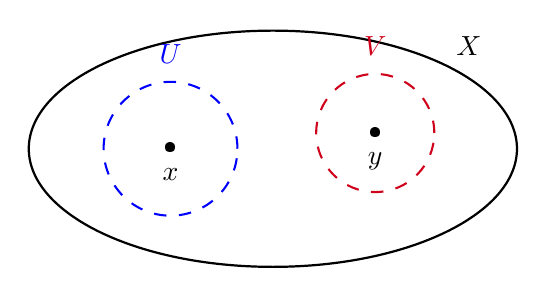
\begin{tikzpicture}[scale=1.0]
    \draw[thick] (0,0) ellipse (3.1 and 1.5);
    \node[anchor=south west] at (2.2,1.05) {$X$};
    \node at (-1.3,0) {\textbullet};
    \node[anchor=north] at (-1.3,-0.12) {$x$};
    \node at (1.3,0.2) {\textbullet};
    \node[anchor=north] at (1.3,0.08) {$y$};
    \draw[color=blue, dash pattern={on 4.5pt off 4.5pt}] (-1.3,0) circle (0.85);
    \draw[color={rgb,255:red,208;green,2;blue,27}, dash pattern={on 4.5pt off 4.5pt}] (1.3,0.2) circle (0.75);
    \node[color=blue, anchor=south] at (-1.3,0.95) {$U$};
    \node[color={rgb,255:red,208;green,2;blue,27}, anchor=south] at (1.3,1.05) {$V$};
\end{tikzpicture}
\end{center}

\begin{proposition}[Metric Spaces are Hausdorff]
    Every metrizable topological space is Hausdorff.
\end{proposition}
\begin{proof}
    Let $d$ be a metric inducing the topology, and let $x \neq y$. Set $r = d(x, y)/2 > 0$. Then $U = D_r(x)$ and $V = D_r(y)$ are open sets containing $x$ and $y$ respectively, and they are disjoint: if $z \in U \cap V$ then $d(x, y) \leq d(x, z) + d(z, y) < 2r = d(x, y)$, a contradiction.
\end{proof}

\begin{example}[Non-Metrizable Topologies]
    The indiscrete topology on a set with at least two points is not Hausdorff (there aren't enough open sets), which gives another proof that it isn't metrizable. Similarly, the cofinite topology on an infinite set is not Hausdorff, since any two non-empty open sets intersect -- so it is not metrizable either.
\end{example}

\subsection{Closed Sets, Neighborhoods and Convergence}

In metric spaces we could define closed sets via convergent sequences, and we then proved that a set is closed if and only if its complement is open. In a general topological space, sequences are no longer expressive enough to detect the topology, so we take the complement property as the \emph{definition}.

\begin{definition}[Closed Set]
    A subset $A$ of a topological space $X$ is \vocab{closed} in $X$ if $X \backslash A$ is open in $X$.
\end{definition}

Taking complements in the axioms for a topology (using De Morgan's laws) immediately gives the following.

\begin{proposition}[Properties of Closed Sets]
    In a topological space $X$:
    \begin{enumerate}[label=(\roman*)]
        \item $\emptyset$ and $X$ are closed;
        \item if $A_i$ is closed for all $i$ in a non-empty index set $I$, then $\bigcap_{i \in I} A_i$ is closed;
        \item if $A, B$ are closed, then $A \cup B$ is closed.
    \end{enumerate}
\end{proposition}

Note that sets are not doors: a set can be open, closed, both (like $\emptyset$), or neither. For example, in a discrete space every set is both open and closed, while in the cofinite topology on an infinite set, the closed sets are exactly the finite sets and the whole space.

\begin{definition}[Neighborhood]
    Let $X$ be a topological space, $x \in X$ and $U \subset X$. We say $U$ is a \vocab{neighborhood} of $x$ in $X$ if there is an open set $V$ with $x \in V \subset U$.
\end{definition}

This matches our characterisation of neighborhoods in metric spaces. Just as before, open sets are precisely the sets that are neighborhoods of all of their points.

\begin{proposition}
    A subset $U$ of a topological space $X$ is open if and only if $U$ is a neighborhood of every $x \in U$.
\end{proposition}
\begin{proof}
    If $U$ is open and $x \in U$, then $V = U$ witnesses that $U$ is a neighborhood of $x$. Conversely, if for each $x \in U$ there's an open $V_x$ with $x \in V_x \subset U$, then $U = \bigcup_{x \in U} V_x$ is a union of open sets, hence open.
\end{proof}

We can also define convergence, mimicking the neighborhood description of convergence that we proved for metric spaces.

\begin{definition}[Convergence]
    A sequence $x_n$ in a topological space $X$ \vocab{converges} to $x \in X$ if for every neighborhood $U$ of $x$, there is some $N \in \N$ such that $x_n \in U$ for all $n \geq N$. We write $x_n \rightarrow x$.
\end{definition}

It is equivalent to only require this for every \emph{open} $U$ containing $x$ (any neighborhood contains such an open set). In metric spaces, this recovers exactly our old definition. In general topological spaces, however, convergence can behave very oddly.

\begin{example}[Convergence Can Be Strange]
    In an indiscrete topological space $X$, the only neighborhood of any point is $X$ itself, so \emph{every} sequence converges to \emph{every} point.

    In the cofinite topology on an infinite set $X$, a sequence $x_n$ converges to $x$ if and only if for each $y \neq x$, the set $\{n \mid x_n = y\}$ is finite. In particular, a sequence of \emph{distinct} points converges to every point of $X$ at once.
\end{example}

The property needed to rule out this behaviour and make limits unique is precisely the Hausdorff property.

\begin{proposition}[Uniqueness of Limits in Hausdorff Spaces]
    Let $X$ be a Hausdorff topological space. If $x_n \rightarrow x$ and $x_n \rightarrow y$ in $X$, then $x = y$.
\end{proposition}
\begin{proof}
    Suppose $x \neq y$. Then there are disjoint open sets $U \ni x$ and $V \ni y$. Since $x_n \rightarrow x$ there is $N_1$ with $x_n \in U$ for $n \geq N_1$, and since $x_n \rightarrow y$ there is $N_2$ with $x_n \in V$ for $n \geq N_2$. But then for $n \geq \max\{N_1, N_2\}$ we have $x_n \in U \cap V = \emptyset$, a contradiction.
\end{proof}

\begin{remark}
    In a metric space, we characterised closed sets as those closed under taking limits of sequences. In a general topological space only one direction survives: if $A$ is closed, $x_n \in A$ and $x_n \rightarrow x$, then $x \in A$ (otherwise $X \backslash A$ would be an open neighborhood of $x$ containing some $x_n$). But there are non-closed sets that are closed under limits -- sequences are simply too short-sighted to see all of a general topology.
\end{remark}

\subsection{Interiors, Closures and Density}

Given an arbitrary subset $A$ of a topological space, there is a canonical way to `round it down' to an open set, and to `round it up' to a closed one.

\begin{definition}[Interior and Closure]
    Let $X$ be a topological space and $A \subset X$. The \vocab{interior} of $A$ is
    $$
    A^{\circ} = \bigcup \{U \subset X \mid U \text{ open in } X, \ U \subset A\},
    $$
    and the \vocab{closure} of $A$ is
    $$
    \ol{A} = \bigcap \{F \subset X \mid F \text{ closed in } X, \ F \supset A\}.
    $$
\end{definition}

Since unions of open sets are open, $A^{\circ}$ is open, and it is clearly the \emph{largest} open subset of $A$. Similarly $\ol{A}$ is the smallest closed set containing $A$ (the intersection is over a non-empty family, as $X$ itself is closed). In particular, $A$ is open if and only if $A = A^{\circ}$, and closed if and only if $A = \ol{A}$.

There is a more hands-on description of both.

\begin{proposition}[Pointwise Descriptions]
    Let $X$ be a topological space and $A \subset X$. Then:
    \begin{enumerate}[label=(\roman*)]
        \item $A^{\circ} = \{x \in X \mid A \text{ is a neighborhood of } x\}$;
        \item $\ol{A} = \{x \in X \mid \text{every neighborhood of } x \text{ meets } A\}$.
    \end{enumerate}
\end{proposition}
\begin{proof}
    \emph{Part (i)}. If $A$ is a neighborhood of $x$, there is an open $U$ with $x \in U \subset A$, so $x \in A^{\circ}$. Conversely if $x \in A^{\circ}$, then $A^{\circ}$ itself is an open set with $x \in A^{\circ} \subset A$.

    \emph{Part (ii)}. Suppose $x \not \in \ol{A}$. Then there is a closed $F \supset A$ with $x \not \in F$, and $U = X \backslash F$ is a neighborhood of $x$ with $U \cap A = \emptyset$. Conversely, suppose some neighborhood $U$ of $x$ misses $A$. Shrinking, we may take $U$ open. Then $F = X \backslash U$ is closed and contains $A$, so $\ol{A} \subset F$, and since $x \not \in F$ we get $x \not \in \ol{A}$.
\end{proof}

\begin{example}
    In $\R$, take $A = [0, 1) \cup \{2\}$. Then $A^{\circ} = (0, 1)$ and $\ol{A} = [0, 1] \cup \{2\}$. For the rationals, $\Q^{\circ} = \emptyset$ (every interval contains irrationals) and $\ol{\Q} = \R$ (every interval contains rationals). For the integers, $\Z^{\circ} = \emptyset$ and $\ol{\Z} = \Z$.
\end{example}

\begin{remark}
    In a \emph{metric} space, $x \in \ol{A}$ if and only if there is a sequence in $A$ converging to $x$ (take $x_n \in D_{1/n}(x) \cap A$). In a general topological space, having such a sequence still implies $x \in \ol{A}$, but the converse can fail.
\end{remark}

\begin{definition}[Dense and Separable]
    A subset $A$ of a topological space $X$ is \vocab{dense} in $X$ if $\ol{A} = X$. We say $X$ is \vocab{separable} if it has a countable dense subset.
\end{definition}

\begin{example}
    $\R^n$ is separable, since $\Q^n$ is countable and dense. An uncountable set with the discrete topology is \emph{not} separable, since every subset is closed and so the only dense subset is the whole space.
\end{example}

\subsection{Subspaces}

If $Y$ is a subset of a topological space $X$, then $Y$ inherits a topology from $X$ in a natural way.

\begin{definition}[Subspace Topology]
    Let $(X, \tau)$ be a topological space and $Y \subset X$. The \vocab{subspace topology} on $Y$ is
    $$
    \tau|_Y = \{V \cap Y \mid V \in \tau\}.
    $$
\end{definition}

It's easy to check that this is a topology (intersecting with $Y$ commutes with unions and intersections). Note that a set open in $Y$ need not be open in $X$.

\begin{example}
    Let $X = \R$, $Y = [0, 2]$ and $U = (1, 2]$. Then $U = (1, 3) \cap Y$ is open in $Y$, but $U$ is certainly not open in $\R$ -- no interval around $2$ fits inside $U$.
\end{example}

\begin{remark}
    Reassuringly, the constructions we already have are all consistent with each other:
    \begin{enumerate}[label=(\roman*)]
        \item If $Z \subset Y \subset X$, the subspace topology that $Z$ inherits from $Y$ (with its subspace topology) is the same as the one it inherits directly from $X$.
        \item If $(M, d)$ is a metric space and $N \subset M$, then the metric topology of the metric subspace $(N, d)$ coincides with the subspace topology induced by the metric topology of $M$. This is because balls in $N$ are exactly balls of $M$ intersected with $N$.
    \end{enumerate}
\end{remark}

Closed sets in a subspace have exactly the description you'd hope for.

\begin{proposition}[Closed Sets and Closures in Subspaces]
    Let $X$ be a topological space, $A \subset Y \subset X$. Then $A$ is closed in $Y$ if and only if $A = B \cap Y$ for some closed $B$ in $X$. Moreover, writing $\operatorname{cl}_Y$ for closure inside the space $Y$,
    $$
    \operatorname{cl}_Y(A) = \ol{A} \cap Y,
    $$
    where $\ol{A}$ denotes closure in $X$.
\end{proposition}
\begin{proof}
    For the first claim, $A$ is closed in $Y$ if and only if $Y \backslash A$ is open in $Y$, that is, $Y \backslash A = V \cap Y$ for some open $V$ in $X$. Taking $B = X \backslash V$, this says exactly $A = B \cap Y$ with $B$ closed in $X$.

    For the second, $\ol{A} \cap Y$ is closed in $Y$ by the first part and contains $A$, so $\operatorname{cl}_Y(A) \subset \ol{A} \cap Y$. Conversely, write $\operatorname{cl}_Y(A) = B \cap Y$ with $B$ closed in $X$. Then $A \subset B$, so $\ol{A} \subset B$, and hence $\ol{A} \cap Y \subset B \cap Y = \operatorname{cl}_Y(A)$.
\end{proof}

The corresponding statement for interiors is \emph{false} in general -- for example, with $A = Y = \{0\}$ inside $X = \R$, we have $\operatorname{int}_Y(A) = \{0\}$ but $A^{\circ} = \emptyset$ in $\R$.

\subsection{Continuity and Homeomorphisms}

Our characterisation of global continuity in metric spaces -- preimages of open sets are open -- becomes the \emph{definition} of continuity for topological spaces.

\begin{definition}[Continuity]
    A function $f: X \rightarrow Y$ between topological spaces is \vocab{continuous} if for every open set $V$ in $Y$, the preimage $f^{-1}(V)$ is open in $X$.
\end{definition}

For metric spaces this agrees with the $\varepsilon$--$\delta$ definition, by our earlier work. Let's collect the basic properties.

\begin{proposition}[Basic Properties of Continuity]
    Let $f: X \rightarrow Y$ and $g: Y \rightarrow Z$ be functions between topological spaces.
    \begin{enumerate}[label=(\roman*)]
        \item Constant functions are continuous, and the identity $\operatorname{id}: X \rightarrow X$ is continuous.
        \item $f$ is continuous if and only if $f^{-1}(B)$ is closed in $X$ for every closed $B$ in $Y$.
        \item If $f$ and $g$ are continuous, then so is $g \circ f$.
        \item If $Y \subset X$ has the subspace topology, the inclusion $i: Y \rightarrow X$ is continuous, and hence if $f: X \rightarrow Z$ is continuous, so is the restriction $f|_Y = f \circ i$.
    \end{enumerate}
\end{proposition}
\begin{proof}
    \emph{Part (i)}. If $f(x) = y_0$ for all $x$, then $f^{-1}(V)$ is $X$ or $\emptyset$ depending on whether $y_0 \in V$, and both are open. For the identity, $\operatorname{id}^{-1}(V) = V$.

    \emph{Part (ii)}. This follows from $f^{-1}(Y \backslash B) = X \backslash f^{-1}(B)$, together with the fact that a set is open if and only if its complement is closed.

    \emph{Part (iii)}. For open $W \subset Z$, we have $(g \circ f)^{-1}(W) = f^{-1}(g^{-1}(W))$, which is open since $g^{-1}(W)$ is open by the continuity of $g$, and preimages of open sets under $f$ are open.

    \emph{Part (iv)}. For open $V$ in $X$, $i^{-1}(V) = V \cap Y$, which is open in $Y$ by the definition of the subspace topology.
\end{proof}

\begin{definition}[Homeomorphism]
    A function $f: X \rightarrow Y$ between topological spaces is a \vocab{homeomorphism} if $f$ is a bijection and both $f$ and $f^{-1}$ are continuous. If such an $f$ exists we say $X$ and $Y$ are \vocab{homeomorphic}, written $X \cong Y$.
\end{definition}

A homeomorphism induces a bijection between the topologies of $X$ and $Y$, so homeomorphic spaces are indistinguishable as topological spaces. This makes the following notion the central `sameness' concept of the subject.

\begin{definition}[Topological Property]
    A property $\mathcal{P}$ of topological spaces is a \vocab{topological property} (or \vocab{topological invariant}) if whenever $X \cong Y$, the space $X$ has property $\mathcal{P}$ if and only if $Y$ does.
\end{definition}

\begin{example}
    Being Hausdorff, being metrizable and being separable are all topological properties. On the other hand, being \emph{complete} with respect to a specific metric is not: $\R \cong (0, 1)$ as topological spaces, but the usual metric on $\R$ is complete while the usual metric on $(0, 1)$ is not. Completeness is a property of a metric, not of a topology.
\end{example}

Much of the power of topological invariants is in proving that spaces are \emph{not} homeomorphic -- if we can find a topological property that one space has and another lacks, no homeomorphism can exist. We'll see genuinely useful invariants (connectedness and compactness) in the coming sections.

\begin{definition}[Open Map]
    A function $f: X \rightarrow Y$ is an \vocab{open map} if $f(U)$ is open in $Y$ for every open $U$ in $X$.
\end{definition}

If $f$ is a bijection, then $f^{-1}$ is continuous exactly when $f$ is an open map (since $(f^{-1})^{-1}(U) = f(U)$). So the homeomorphisms are exactly the continuous open bijections.

\subsection{Products}

Given topological spaces $X$ and $Y$, we want a sensible topology on the product $X \times Y$. Certainly if $U$ is open in $X$ and $V$ is open in $Y$, we would like the `open box' $U \times V$ to be open in $X \times Y$. Boxes are closed under finite intersections, since
$$
(U \times V) \cap (U' \times V') = (U \cap U') \times (V \cap V'),
$$
but a union of boxes need not be a box, so we must throw the unions in too. That is, we take the boxes as a \emph{basis}.

\begin{definition}[Product Topology]
    Let $X$ and $Y$ be topological spaces. The \vocab{product topology} on $X \times Y$ is the topology whose open sets are the sets of the form
    $$
    W = \bigcup_{i \in I} U_i \times V_i,
    $$
    where each $U_i$ is open in $X$ and each $V_i$ is open in $Y$.
\end{definition}

Equivalently, $W \subset X \times Y$ is open if and only if for every $(x, y) \in W$ there are open sets $U \ni x$ in $X$ and $V \ni y$ in $Y$ with $U \times V \subset W$.

We should immediately check this is consistent with what we already do for metric spaces.

\begin{example}[Products of Metric Spaces]
    Let $(M, d)$ and $(M', d')$ be metric spaces, and consider the product metric $d_{\infty}$ on $M \times M'$ (recall all the product metrics $d_1, d_2, d_{\infty}$ are Lipschitz equivalent, so induce the same topology). For $z = (x, x')$ and $r > 0$,
    $$
    D_r(z) = \{(y, y') \mid d(x, y) < r \text{ and } d'(x', y') < r\} = D_r(x) \times D_r(x'),
    $$
    so open balls in $d_\infty$ are precisely `square' boxes. It follows easily that a subset of $M \times M'$ is $d_{\infty}$-open if and only if it is open in the product topology -- the two constructions agree. In particular, the product topology on $\R \times \R$ is the usual Euclidean topology on $\R^2$.
\end{example}

The product topology is `designed' to make the coordinate projections behave well, in the following precise sense.

\begin{proposition}[Continuity and Products]
    Let $X, Y$ be topological spaces and give $X \times Y$ the product topology. Write $q_X: X \times Y \rightarrow X$ and $q_Y: X \times Y \rightarrow Y$ for the coordinate projections. Then:
    \begin{enumerate}[label=(\roman*)]
        \item $q_X$ and $q_Y$ are continuous;
        \item for any topological space $Z$, a function $g: Z \rightarrow X \times Y$ is continuous if and only if both $q_X \circ g$ and $q_Y \circ g$ are continuous.
    \end{enumerate}
\end{proposition}
\begin{proof}
    \emph{Part (i)}. For open $U$ in $X$, we have $q_X^{-1}(U) = U \times Y$, a box, hence open. Similarly for $q_Y$.

    \emph{Part (ii)}. If $g$ is continuous then $q_X \circ g$ and $q_Y \circ g$ are compositions of continuous maps. Conversely, suppose $h = q_X \circ g$ and $k = q_Y \circ g$ are continuous, so that $g(z) = (h(z), k(z))$. For open sets $U$ in $X$ and $V$ in $Y$,
    $$
    g^{-1}(U \times V) = h^{-1}(U) \cap k^{-1}(V),
    $$
    which is open in $Z$. A general open set $W$ in $X \times Y$ is a union of boxes $\bigcup_{i} U_i \times V_i$, so $g^{-1}(W) = \bigcup_i g^{-1}(U_i \times V_i)$ is a union of open sets, hence open.
\end{proof}

In other words, a map \emph{into} a product is continuous exactly when its components are. This all extends to finite products $X_1 \times \cdots \times X_n$ in the obvious way, with basis the boxes $U_1 \times \cdots \times U_n$. If each $X_i$ is metrizable, so is the product, using for example the $d_{\infty}$ metric.

\subsection{Quotients}

Products let us build bigger spaces from smaller ones; \emph{quotients} let us build new spaces by \emph{gluing}. The setup is a topological space $X$ together with an equivalence relation $R$ on $X$ (we write $x \sim y$ for $(x, y) \in R$). We write $X/R$ for the set of equivalence classes, and $q: X \rightarrow X/R$ for the \vocab{quotient map} sending each point to its equivalence class. The idea is that in $X/R$, equivalent points of $X$ have been glued into a single point.

\begin{definition}[Quotient Topology]
    Let $X$ be a topological space and $R$ an equivalence relation on $X$. The \vocab{quotient topology} on $X/R$ is
    $$
    \tau = \{V \subset X/R \mid q^{-1}(V) \text{ is open in } X\}.
    $$
\end{definition}

This is a topology because taking preimages commutes with unions and intersections: $q^{-1}(\emptyset) = \emptyset$, $q^{-1}(X/R) = X$, $q^{-1}(\bigcup V_i) = \bigcup q^{-1}(V_i)$ and $q^{-1}(U \cap V) = q^{-1}(U) \cap q^{-1}(V)$. Note that $q$ is continuous by construction -- indeed the quotient topology is the \emph{finest} topology on $X/R$ making $q$ continuous.

\begin{example}[The Circle as a Quotient]
    Consider $\R$ with the equivalence relation $x \sim y$ if and only if $x - y \in \Z$, giving the quotient $\R / \Z$. Every real number is equivalent to one in $[0, 1]$, and the only identification within $[0, 1]$ is that $0 \sim 1$. So $\R/\Z$ is the interval $[0, 1]$ with its two endpoints glued together -- which should be a circle! We will prove that $\R/\Z \cong S^1$ once we have compactness available, which makes the proof essentially effortless.
\end{example}

\begin{example}[Quotients Can Be Horrible]
    Let $x \sim y$ if and only if $x - y \in \Q$, and consider $\R / \Q$. If $V \subset \R/\Q$ is open and non-empty, then $q^{-1}(V)$ is open and non-empty, so contains an interval $(a, b)$. But then given \emph{any} $x \in \R$, we can pick a rational $r \in (a - x, b - x)$, and then $x + r \in (a, b)$, so $q(x) = q(x + r) \in V$. Hence $V = \R/\Q$, and the quotient topology on $\R/\Q$ is indiscrete!

    In particular, quotients of metrizable spaces (indeed, of $\R$ itself) can fail to be Hausdorff or metrizable. Quotients require some care.
\end{example}

\begin{example}[Gluing a Square]
    Let $Q = [0, 1] \times [0, 1] \subset \R^2$. Identifying the left and right edges of $Q$ via $(0, y) \sim (1, y)$ rolls the square up into a \emph{cylinder}. If we additionally identify the top and bottom edges via $(x, 0) \sim (x, 1)$ (and consequently all four corners become one point), we get the \vocab{torus} -- the surface of a doughnut. The picture to have in mind is:

    \begin{center}
    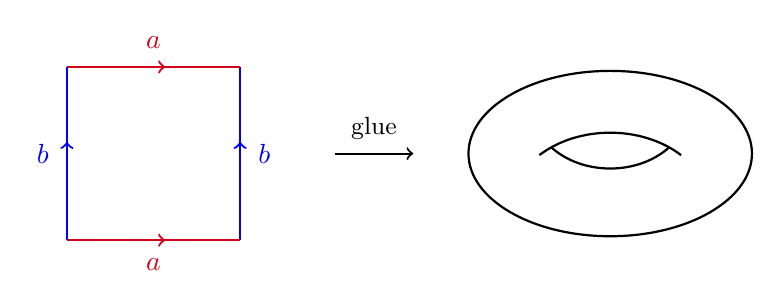
\begin{tikzpicture}[scale=1.0]
        \draw[thick, color=blue] (0,0) -- (0,2.2);
        \draw[thick, color=blue] (2.2,0) -- (2.2,2.2);
        \draw[thick, color={rgb,255:red,208;green,2;blue,27}] (0,0) -- (2.2,0);
        \draw[thick, color={rgb,255:red,208;green,2;blue,27}] (0,2.2) -- (2.2,2.2);
        \draw[->, thick, color=blue] (0,1.0) -- (0,1.25);
        \draw[->, thick, color=blue] (2.2,1.0) -- (2.2,1.25);
        \draw[->, thick, color={rgb,255:red,208;green,2;blue,27}] (1.0,0) -- (1.25,0);
        \draw[->, thick, color={rgb,255:red,208;green,2;blue,27}] (1.0,2.2) -- (1.25,2.2);
        \node[color=blue, anchor=east] at (-0.1,1.1) {$b$};
        \node[color=blue, anchor=west] at (2.3,1.1) {$b$};
        \node[color={rgb,255:red,208;green,2;blue,27}, anchor=north] at (1.1,-0.1) {$a$};
        \node[color={rgb,255:red,208;green,2;blue,27}, anchor=south] at (1.1,2.3) {$a$};
        \draw[->] (3.4,1.1) -- (4.4,1.1);
        \node[anchor=south] at (3.9,1.15) {\small glue};
        \begin{scope}[shift={(6.9,1.1)}]
            \draw[thick] (0,0) ellipse (1.8 and 1.05);
            \draw[thick] (-0.75,0.08) .. controls (-0.35,-0.28) and (0.35,-0.28) .. (0.75,0.08);
            \draw[thick] (-0.9,-0.02) .. controls (-0.4,0.36) and (0.4,0.36) .. (0.9,-0.02);
        \end{scope}
    \end{tikzpicture}
    \end{center}

    Formally, the resulting quotient $Q/R$ is homeomorphic to $\R^2/\Z^2$ (quotienting by the relation $x \sim y \iff x - y \in \Z^2$), and also to the familiar torus surface embedded in $\R^3$.
\end{example}

To actually \emph{work} with quotients, the key tool is the way that maps out of $X$ descend to maps out of $X/R$.

\begin{proposition}[Factoring Maps Through Quotients]
    Let $X$ be a set, $R$ an equivalence relation on $X$, and $q: X \rightarrow X/R$ the quotient map. Let $f: X \rightarrow Y$ be a function which \vocab{respects} $R$, meaning $x \sim y$ implies $f(x) = f(y)$. Then there is a unique map $\tilde{f}: X/R \rightarrow Y$ such that $f = \tilde{f} \circ q$.

    Moreover $\tilde{f}$ has the same image as $f$, and if $f$ \vocab{fully respects} $R$, meaning $x \sim y \iff f(x) = f(y)$, then $\tilde{f}$ is injective.
\end{proposition}
\begin{proof}
    Any class $z \in X/R$ is $q(x)$ for some $x$, and the requirement $\tilde{f}(q(x)) = f(x)$ pins down $\tilde{f}(z)$ -- this is well defined precisely because $f$ respects $R$. Uniqueness and the image claim follow since $q$ is surjective. If $f$ fully respects $R$ and $\tilde{f}(q(x)) = \tilde{f}(q(y))$, then $f(x) = f(y)$, so $x \sim y$ and $q(x) = q(y)$, giving injectivity.
\end{proof}

\begin{proposition}[Continuity of Factored Maps]
    In the setting above, suppose additionally that $X$ and $Y$ are topological spaces and that $X/R$ carries the quotient topology. Then:
    \begin{enumerate}[label=(\roman*)]
        \item if $f$ is continuous, then so is $\tilde{f}$;
        \item if $f$ is an open map, then so is $\tilde{f}$.
    \end{enumerate}
    In particular, if $f$ is a continuous surjection that fully respects $R$, then $\tilde{f}$ is a continuous bijection, and if $f$ is additionally an open map, then $\tilde{f}$ is a homeomorphism $X/R \cong Y$.
\end{proposition}
\begin{proof}
    \emph{Part (i)}. For open $V$ in $Y$,
    $$
    q^{-1}(\tilde{f}^{-1}(V)) = (\tilde{f} \circ q)^{-1}(V) = f^{-1}(V),
    $$
    which is open in $X$, so by the definition of the quotient topology, $\tilde{f}^{-1}(V)$ is open in $X/R$.

    \emph{Part (ii)}. Let $V$ be open in $X/R$, and set $U = q^{-1}(V)$, which is open in $X$. Since $q$ is surjective, $q(U) = V$, so
    $$
    \tilde{f}(V) = \tilde{f}(q(U)) = f(U),
    $$
    which is open in $Y$ since $f$ is an open map.
\end{proof}

Finally, let us record when a quotient has a chance of being Hausdorff. Thinking of $R$ as a subset of $X \times X$ (with the product topology), we have the following.

\begin{proposition}[Hausdorff Quotients]
    Let $X$ be a topological space and $R$ an equivalence relation on $X$.
    \begin{enumerate}[label=(\roman*)]
        \item If $X/R$ is Hausdorff, then $R$ is closed in $X \times X$.
        \item If $R$ is closed in $X \times X$ and $q$ is an open map, then $X/R$ is Hausdorff.
    \end{enumerate}
\end{proposition}
\begin{proof}
    \emph{Part (i)}. Let $W = (X \times X) \backslash R$; we show $W$ is open. Given $(x, y) \in W$ we have $q(x) \neq q(y)$, so there are disjoint open sets $S \ni q(x)$ and $T \ni q(y)$ in $X/R$. Then $U = q^{-1}(S)$ and $V = q^{-1}(T)$ are open in $X$ with $x \in U$, $y \in V$, and for any $(a, b) \in U \times V$ we have $q(a) \in S$ and $q(b) \in T$, so $q(a) \neq q(b)$, that is, $a \not\sim b$. Hence $(x, y) \in U \times V \subset W$, and $W$ is open.

    \emph{Part (ii)}. Let $z \neq w$ in $X/R$, and pick $x, y \in X$ with $q(x) = z$, $q(y) = w$. Then $x \not\sim y$, so $(x, y)$ lies in the open set $W = (X \times X) \backslash R$, and there are open sets $U \ni x$, $V \ni y$ with $U \times V \subset W$. Since $q$ is an open map, $q(U)$ and $q(V)$ are open, and they contain $z$ and $w$ respectively. They are disjoint: if $q(a) = q(b)$ with $a \in U$, $b \in V$, then $(a, b) \in R \cap (U \times V)$, contradicting $U \times V \subset W$. So $X/R$ is Hausdorff.
\end{proof}

\section{Connectedness}

We now come to our first substantial topological property. Recall the intermediate value theorem from Analysis I: a continuous function on an interval takes all values between any two of its values. Which feature of intervals makes this work? Intuitively, an interval is `all in one piece' -- and this is the idea we now make precise, for arbitrary topological spaces.

\subsection{Connected Spaces}

\begin{definition}[Connected]
    A topological space $X$ is \vocab{disconnected} if there exist open sets $U, V$ in $X$ such that
    $$
    U \cap V = \emptyset, \quad U \cup V = X, \quad U, V \neq \emptyset.
    $$
    In this case we say $U$ and $V$ \vocab{disconnect} $X$. We say $X$ is \vocab{connected} if it is not disconnected.
\end{definition}

\begin{center}
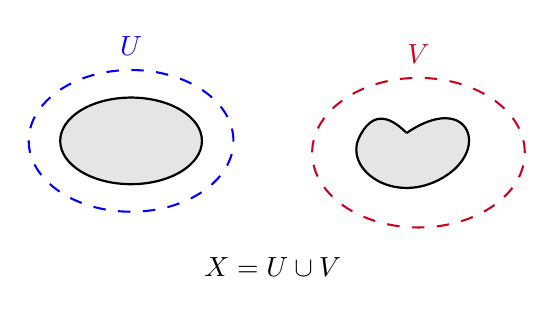
\begin{tikzpicture}[scale=1.0]
    \draw[thick, fill=lightgray, fill opacity=0.4] (-1.75,0) ellipse (0.9 and 0.55);
    \draw[thick, fill=lightgray, fill opacity=0.4] (1.75,0.1) .. controls (2.55,0.65) and (2.85,-0.15) .. (2.15,-0.5) .. controls (1.55,-0.8) and (0.95,-0.35) .. (1.15,0.05) .. controls (1.3,0.35) and (1.5,0.35) .. (1.75,0.1);
    \draw[color=blue, dash pattern={on 4.5pt off 4.5pt}] (-1.75,0) ellipse (1.3 and 0.9);
    \draw[color={rgb,255:red,208;green,2;blue,27}, dash pattern={on 4.5pt off 4.5pt}] (1.9,-0.15) ellipse (1.35 and 0.95);
    \node[color=blue, anchor=south] at (-1.75,0.95) {$U$};
    \node[color={rgb,255:red,208;green,2;blue,27}, anchor=south] at (1.9,0.85) {$V$};
    \node[anchor=north] at (0.05,-1.35) {$X = U \cup V$};
\end{tikzpicture}
\end{center}

Equivalently (taking complements), $X$ is disconnected if and only if it has a subset which is open, closed, non-empty and not the whole space.

There is a slick reformulation of connectedness in terms of continuous functions, which is frequently the easiest version to use in proofs. Here $\Z$ carries the subspace topology from $\R$, which is its discrete topology.

\begin{theorem}[Characterisations of Connectedness]\label{thm:connchar}
    Let $X$ be a topological space. The following are equivalent:
    \begin{enumerate}[label=(\roman*)]
        \item $X$ is connected;
        \item if $f: X \rightarrow \R$ is continuous, then $f(X)$ is an interval;
        \item every continuous function $f: X \rightarrow \Z$ is constant.
    \end{enumerate}
\end{theorem}
\begin{proof}
    \emph{(i) implies (ii)}. Suppose $f: X \rightarrow \R$ is continuous but $f(X)$ is not an interval. Then there are $a < b < c$ with $a, c \in f(X)$ but $b \not \in f(X)$. Let $U = f^{-1}((-\infty, b))$ and $V = f^{-1}((b, \infty))$. These are open (preimages of open sets), disjoint, non-empty (they contain points mapping to $a$ and $c$), and since $b$ is not a value of $f$ their union is all of $X$. So $U, V$ disconnect $X$, a contradiction.

    \emph{(ii) implies (iii)}. If $f: X \rightarrow \Z$ is continuous, then viewed as a map into $\R$ it is continuous, so $f(X)$ is an interval consisting of integers -- which must be a single point.

    \emph{(iii) implies (i)}. Suppose $U, V$ disconnect $X$. Define $f: X \rightarrow \Z$ by $f = 0$ on $U$ and $f = 1$ on $V$. For any $W \subset \Z$, the preimage $f^{-1}(W)$ is one of $\emptyset, U, V, X$, all of which are open, so $f$ is continuous. But $f$ is not constant, contradicting (iii).
\end{proof}

We can now identify the connected subsets of the real line. Here, and always, a subset of a topological space is called connected if it is connected in its subspace topology. Recall that $I \subset \R$ is an \vocab{interval} if whenever $x < y < z$ with $x, z \in I$, we have $y \in I$.

\begin{theorem}[Connected Subsets of $\R$]
    A subset $X \subset \R$ is connected if and only if $X$ is an interval.
\end{theorem}
\begin{proof}
    If $X$ is connected, then the inclusion $i: X \rightarrow \R$ is continuous, so $X = i(X)$ is an interval by the theorem above.

    Conversely, suppose $X$ is an interval and $f: X \rightarrow \R$ is continuous. If $x < y$ are points of $X$ then $[x, y] \subset X$, and by the intermediate value theorem from Analysis I, $f$ takes every value between $f(x)$ and $f(y)$ on $[x, y]$. Hence $f(X)$ is an interval, and by the theorem above, $X$ is connected.
\end{proof}

Note the pleasing exchange that has taken place here: the intermediate value theorem told us that intervals are connected, and conversely, once we know a space is connected, part (ii) of Theorem~\ref{thm:connchar} \emph{is} the intermediate value theorem for that space.

\begin{example}
    Any indiscrete space is connected (there aren't enough open sets to disconnect it). The cofinite topology on an infinite set is connected (any two non-empty open sets meet). A discrete space with at least two points is disconnected.
\end{example}

When working with subspaces, it's convenient to phrase disconnection using open sets of the ambient space.

\begin{lemma}[Disconnecting Subspaces]
    Let $Y$ be a subspace of a topological space $X$. Then $Y$ is disconnected if and only if there are open sets $U, V$ in $X$ such that
    $$
    U \cap V \cap Y = \emptyset, \quad Y \subset U \cup V, \quad U \cap Y \neq \emptyset, \quad V \cap Y \neq \emptyset.
    $$
    In this situation we say that $U$ and $V$ disconnect $Y$ in $X$.
\end{lemma}
\begin{proof}
    Open subsets of $Y$ are exactly the sets $U \cap Y$ for $U$ open in $X$, so this is just unwinding the definition of the subspace topology.
\end{proof}

\begin{proposition}[Closures of Connected Sets]\label{prop:closureconn}
    Let $Y$ be a connected subspace of a topological space $X$. Then $\ol{Y}$ is connected. More generally, any $Z$ with $Y \subset Z \subset \ol{Y}$ is connected.
\end{proposition}
\begin{proof}
    Suppose $U, V$ are open in $X$ and disconnect $Z$. Since $Y \subset Z$, we have $U \cap V \cap Y = \emptyset$ and $Y \subset U \cup V$. If both $U \cap Y$ and $V \cap Y$ were non-empty, then $U, V$ would disconnect $Y$, which is connected -- so without loss of generality $V \cap Y = \emptyset$. Then $Y \subset X \backslash V$, which is closed, so $\ol{Y} \subset X \backslash V$, and hence $V \cap Z \subset V \cap \ol{Y} = \emptyset$. This contradicts $U, V$ disconnecting $Z$.
\end{proof}

\begin{theorem}[Continuous Images of Connected Spaces]
    Let $f: X \rightarrow Y$ be a continuous function between topological spaces. If $X$ is connected, then $f(X)$ is connected.
\end{theorem}
\begin{proof}
    Suppose $U, V$ are open in $Y$ and disconnect $f(X)$. Then $f^{-1}(U)$ and $f^{-1}(V)$ are open in $X$, they are non-empty (as $U$ and $V$ meet $f(X)$), their union is $X$ (as $f(X) \subset U \cup V$), and they are disjoint (if $x$ was in both, $f(x) \in U \cap V \cap f(X) = \emptyset$). So they disconnect $X$, a contradiction.
\end{proof}

In particular, connectedness is a topological property, and any quotient of a connected space is connected (the quotient map is a continuous surjection).

\begin{lemma}[Unions of Overlapping Connected Sets]\label{lemma:unions}
    Let $\mathcal{A}$ be a family of connected subsets of a topological space $X$ such that $A \cap B \neq \emptyset$ for all $A, B \in \mathcal{A}$. Then $\bigcup_{A \in \mathcal{A}} A$ is connected.
\end{lemma}
\begin{proof}
    Let $Y = \bigcup_{A \in \mathcal{A}} A$ and let $f: Y \rightarrow \Z$ be continuous; by Theorem~\ref{thm:connchar} it's enough to show $f$ is constant. For each $A \in \mathcal{A}$, the restriction $f|_A$ is continuous, so it is constant since $A$ is connected. For any $A, B \in \mathcal{A}$, picking a point of $A \cap B$ shows these constants agree. Hence $f$ is constant on $Y$.
\end{proof}

\begin{theorem}[Products of Connected Spaces]
    If $X$ and $Y$ are connected topological spaces, then $X \times Y$ is connected.
\end{theorem}
\begin{proof}
    We may assume both are non-empty. Fix $x_0 \in X$. The map $y \mapsto (x_0, y)$ is continuous (its components are constant and the identity), so its image $\{x_0\} \times Y$ is connected; similarly each $X \times \{y\}$ is connected. Now for $y \in Y$, let
    $$
    A_y = (\{x_0\} \times Y) \cup (X \times \{y\}).
    $$
    The two pieces meet in the point $(x_0, y)$, so each $A_y$ is connected by Lemma~\ref{lemma:unions}. Furthermore, any two $A_y, A_z$ contain $\{x_0\} \times Y$, so they pairwise intersect, and hence
    $$
    \bigcup_{y \in Y} A_y = X \times Y
    $$
    is connected, again by Lemma~\ref{lemma:unions}.
\end{proof}

\begin{example}
    $\R^n$ is connected for every $n$, being a product of copies of the interval $\R$.
\end{example}

\subsection{Path-Connectedness}

There is a second, more intuitive notion of being `all in one piece': you can walk from any point to any other without leaving the space.

\begin{definition}[Path]
    Let $X$ be a topological space and $x, y \in X$. A \vocab{path} from $x$ to $y$ in $X$ is a continuous function $\gamma: [0, 1] \rightarrow X$ with $\gamma(0) = x$ and $\gamma(1) = y$. We say $X$ is \vocab{path-connected} if for all $x, y \in X$ there is a path from $x$ to $y$ in $X$.
\end{definition}

\begin{example}[Convex Sets are Path-Connected]
    Any convex subset $C \subset \R^n$ (one containing the straight line segment between any two of its points) is path-connected: for $y, z \in C$ take the straight-line path $\gamma(t) = (1 - t)y + tz$, which is continuous with image in $C$. In particular open balls $D_r(x)$ are path-connected, since for $y, z \in D_r(x)$,
    $$
    \norm{\gamma(t) - x} = \norm{(1-t)(y - x) + t(z - x)} \leq (1 - t)\norm{y - x} + t\norm{z - x} < r.
    $$
\end{example}

\begin{theorem}[Path-Connected Implies Connected]
    If a topological space $X$ is path-connected, then $X$ is connected.
\end{theorem}
\begin{proof}
    Suppose $U, V$ disconnect $X$, and take $x \in U$, $y \in V$. Let $\gamma$ be a path from $x$ to $y$. Then $\gamma^{-1}(U)$ and $\gamma^{-1}(V)$ are open, non-empty (they contain $0$ and $1$), disjoint, and cover $[0, 1]$ -- so they disconnect $[0, 1]$. But $[0, 1]$ is an interval, hence connected, a contradiction.
\end{proof}

The converse is false, and the standard counterexample is important enough to have a name: the \emph{topologist's sine curve}.

\begin{example}[The Topologist's Sine Curve]\label{ex:sinecurve}
    Consider the set
    $$
    X = \underbrace{\left\{ \left(x, \sin \tfrac{1}{x}\right) \;\middle|\; x > 0 \right\}}_{Y} \cup \underbrace{\{(0, y) \mid -1 \leq y \leq 1\}}_{Z} \subset \R^2.
    $$

    \begin{center}
    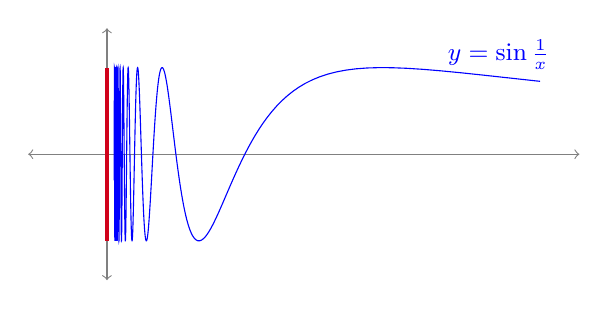
\begin{tikzpicture}[scale=1.0]
        \draw[<->, thin, color=gray] (-1,0) -- (6,0);
        \draw[<->, thin, color=gray] (0,-1.6) -- (0,1.6);
        \draw[thin, samples=800, color=blue] plot[domain=1:60, variable=\t] ({5.5/\t}, {1.1*sin(\t r)});
        \draw[very thick, color={rgb,255:red,208;green,2;blue,27}] (0,-1.1) -- (0,1.1);
        \node[color=blue, anchor=south west] at (4.2,0.95) {\small $y = \sin \frac{1}{x}$};
    \end{tikzpicture}
    \end{center}

    We claim that $X$ is connected but not path-connected.

    \emph{$X$ is connected.} The curve $Y$ is the image of the connected set $(0, \infty)$ under the continuous map $x \mapsto (x, \sin \frac{1}{x})$, so $Y$ is connected. We claim $X = \ol{Y}$; then $X$ is connected by Proposition~\ref{prop:closureconn}. To see $X \subset \ol{Y}$, fix $y \in [-1, 1]$. For each $n$, the map $x \mapsto 1/x$ sends $(0, \frac{1}{n})$ onto $(n, \infty)$, and $\sin$ takes the value $y$ somewhere in any interval of length $2\pi$, so there is $x_n \in (0, \frac{1}{n})$ with $\sin \frac{1}{x_n} = y$. Then $(x_n, y) \in Y$ and $(x_n, y) \rightarrow (0, y)$, so $(0, y) \in \ol{Y}$. Conversely $X$ is closed: if $(x_n, y_n) \in X$ converges to $(x, y)$, then $y \in [-1, 1]$, and either $x = 0$, in which case $(x, y) \in Z \subset X$, or $x > 0$, in which case $x_n > 0$ eventually, so $y_n = \sin\frac{1}{x_n} \rightarrow \sin \frac{1}{x}$ by continuity and $(x, y) \in Y$. Hence $\ol{Y} \subset X$, so $X = \ol{Y}$.

    \emph{$X$ is not path-connected.} Suppose $\gamma = (\gamma_1, \gamma_2): [0, 1] \rightarrow X$ were a path from $(0, 0)$ to $(1, \sin 1)$. The idea is that any path leaving the vertical segment must traverse infinitely many oscillations in finite time. Suppose $\gamma_1(t) > 0$ for some $t$. By the intermediate value theorem, $\gamma_1([0, t]) \supset [0, \gamma_1(t)]$, so for any large $n$ we can find $s < t$ with $\gamma_1(s) = \frac{1}{2\pi n}$, whence $\gamma_2(s) = \sin(2 \pi n) = 0$; and similarly some $s' < t$ with $\gamma_1(s') = \frac{1}{2\pi n + \pi/2}$, whence $\gamma_2(s') = 1$. Iterating this (each time applying the argument on the interval up to the previously found time, with larger $n$), we obtain a decreasing sequence of times $1 \geq t_1 > t_2 > \cdots > 0$ with $\gamma_2(t_k)$ alternating between $0$ and $1$. The sequence $t_k$ is decreasing and bounded below, so it converges to some $t^* \in [0, 1]$; but then $\gamma_2(t_k) \rightarrow \gamma_2(t^*)$ by continuity, which is impossible for a sequence alternating between $0$ and $1$. So no such path exists.
\end{example}

Despite this counterexample, for \emph{open} subsets of Euclidean space the two notions do coincide. First, a lemma that is endlessly useful for building paths (and other functions) piece by piece.

\begin{lemma}[Gluing Lemma]
    Let $X = A \cup B$ be a topological space with $A, B$ closed in $X$, and let $g: A \rightarrow Y$ and $h: B \rightarrow Y$ be continuous functions which agree on $A \cap B$. Then the function $f: X \rightarrow Y$ defined by
    $$
    f(x) = \begin{cases}
        g(x) &\mbox{if } x \in A, \\
        h(x) &\mbox{if } x \in B
       \end{cases}
    $$
    is well defined and continuous.
\end{lemma}
\begin{proof}
    Well-definedness is exactly the agreement on $A \cap B$. Now let $V$ be closed in $Y$. Then
    $$
    f^{-1}(V) = g^{-1}(V) \cup h^{-1}(V),
    $$
    where $g^{-1}(V)$ is closed in $A$, and hence closed in $X$ (it equals $A \cap G$ for some closed $G$ in $X$, and an intersection of closed sets is closed); similarly $h^{-1}(V)$ is closed in $X$. So $f^{-1}(V)$ is closed in $X$ for every closed $V$, and $f$ is continuous.
\end{proof}

With this, being joined by a path is an equivalence relation on any topological space: constant paths give reflexivity, reversing a path ($t \mapsto \gamma(1 - t)$) gives symmetry, and for transitivity we concatenate paths, defining
$$
\eta(t) = \begin{cases}
    \gamma(2t) &\mbox{if } 0 \leq t \leq \frac{1}{2}, \\
    \delta(2t - 1) &\mbox{if } \frac{1}{2} \leq t \leq 1,
   \end{cases}
$$
which is continuous by the gluing lemma applied to $[0, \frac{1}{2}]$ and $[\frac{1}{2}, 1]$. The equivalence classes are called the \vocab{path-connected components} of $X$.

\begin{theorem}[Open Subsets of $\R^n$]\label{thm:openconn}
    Let $U$ be an open subset of $\R^n$. Then $U$ is connected if and only if $U$ is path-connected.
\end{theorem}
\begin{proof}
    Path-connected implies connected always, so suppose $U$ is connected and non-empty, and fix $x_0 \in U$. Let
    $$
    P = \{x \in U \mid \text{there is a path from } x_0 \text{ to } x \text{ in } U\}.
    $$
    We will show $P$ is both open and closed in $U$. Since $U$ is connected and $x_0 \in P \neq \emptyset$, it will follow that $P = U$, which is what we want.

    \emph{$P$ is open.} Let $x \in P$. Since $U$ is open there is $r > 0$ with $D_r(x) \subset U$. Any $y \in D_r(x)$ is joined to $x$ by a straight-line path in $D_r(x)$, and concatenating with a path from $x_0$ to $x$ shows $y \in P$. So $D_r(x) \subset P$.

    \emph{$U \backslash P$ is open.} Let $x \in U \backslash P$, and again take $D_r(x) \subset U$. If some $y \in D_r(x)$ had a path from $x_0$, then concatenating with the segment from $y$ to $x$ would put $x$ in $P$ -- contradiction. So $D_r(x) \subset U \backslash P$.

    Hence $P$ is open and closed in $U$, and $P = U$ as claimed.
\end{proof}

\subsection{Connected Components}

A disconnected space breaks up into natural maximal connected pieces.

\begin{definition}[Connected Component]
    Let $X$ be a topological space. Define a relation on $X$ by $x \sim y$ if and only if there is some connected $A \subset X$ with $x, y \in A$. This is an equivalence relation\footnote{Reflexivity: $\{x\}$ is connected. Symmetry is clear. Transitivity: if $x, y \in A$ and $y, z \in B$ with $A, B$ connected, then $A \cup B$ is connected by Lemma~\ref{lemma:unions} since $y \in A \cap B$, and it contains $x$ and $z$.}, and its equivalence classes are called the \vocab{connected components} of $X$.
\end{definition}

\begin{proposition}[Properties of Components]
    The connected components of a topological space $X$ are precisely the maximal connected subsets of $X$; they are closed, and they partition $X$.
\end{proposition}
\begin{proof}
    That they partition $X$ is immediate as they are equivalence classes. Let $C = C_x$ be the component of $x$.

    \emph{$C$ is connected.} For each $y \in C$ there is a connected $A_y \ni x, y$. Note $A_y \subset C$, since every point of $A_y$ is related to $x$. Then $C = \bigcup_{y \in C} A_y$, the sets $A_y$ pairwise intersect (all contain $x$), so $C$ is connected by Lemma~\ref{lemma:unions}.

    \emph{$C$ is maximal.} If $C \subset A$ with $A$ connected, then every $y \in A$ satisfies $y \sim x$, so $A \subset C$.

    \emph{$C$ is closed.} $\ol{C}$ is connected by Proposition~\ref{prop:closureconn}, so by maximality $\ol{C} = C$.
\end{proof}

\begin{example}
    The components of $\R \backslash \{0\}$ are $(-\infty, 0)$ and $(0, \infty)$. The components of $\Q$ (as a subspace of $\R$) are the singletons: any subset of $\Q$ with two points $p < q$ is disconnected by cutting at an irrational between them. Note this shows components need \emph{not} be open in general.
\end{example}

Since connectedness is a topological invariant, so is the number of connected components, and this gives a genuinely useful way of telling spaces apart. Here is the classic application.

\begin{theorem}[$\R \not\cong \R^n$ for $n \geq 2$]
    For $n \geq 2$, the spaces $\R$ and $\R^n$ are not homeomorphic.
\end{theorem}
\begin{proof}
    Suppose $f: \R \rightarrow \R^n$ were a homeomorphism. Removing a point, $f$ restricts to a homeomorphism from $\R \backslash \{0\}$ to $\R^n \backslash \{f(0)\}$. But $\R \backslash \{0\}$ is disconnected, while $\R^n \backslash \{\text{point}\}$ for $n \geq 2$ is path-connected (any two points can be joined by a path of at most two straight segments avoiding the removed point) and hence connected. This contradicts connectedness being a topological property.
\end{proof}

\begin{remark}
    It is true in general that $\R^m \not\cong \R^n$ for $m \neq n$, but this is substantially harder -- the standard proofs need tools from algebraic topology.
\end{remark}

\section{Compactness}

Our second major topological property is \emph{compactness}. It is best thought of as the topological version of being finite: compact spaces are the ones on which `local' information can always be patched into `global' information using only finitely many patches.

\subsection{Open Covers and Compactness}

To motivate the definition, recall from Analysis I that a continuous function on a closed bounded interval is bounded. Let's think about what makes this work for a continuous $f: X \rightarrow \R$ on a general space. Continuity gives us \emph{local} boundedness for free: every $x \in X$ lies in the open set
$$
U_x = f^{-1}\big((f(x) - 1,\ f(x) + 1)\big),
$$
and $f$ is bounded on $U_x$. The sets $U_x$ cover $X$. If we could always pass to \emph{finitely many} of them, say $U_{x_1}, \dots, U_{x_k}$, still covering $X$, then $f$ would be bounded on all of $X$ by $\max_j |f(x_j)| + 1$. This finite-subcover property is exactly compactness.

\begin{definition}[Open Cover and Compactness]
    Let $X$ be a topological space. An \vocab{open cover} of $X$ is a family $\mathcal{U}$ of open subsets of $X$ with $\bigcup_{U \in \mathcal{U}} U = X$. A \vocab{subcover} of $\mathcal{U}$ is a subfamily $\mathcal{V} \subset \mathcal{U}$ which still covers $X$, and it is a \vocab{finite subcover} if $\mathcal{V}$ is finite.

    We say $X$ is \vocab{compact} if every open cover of $X$ has a finite subcover.
\end{definition}

For a subspace $Y \subset X$, it is easy to check (using the definition of the subspace topology) that $Y$ is compact if and only if every family $\mathcal{U}$ of open sets \emph{of $X$} whose union contains $Y$ admits a finite subfamily whose union still contains $Y$. We use both formulations interchangeably.

\begin{center}
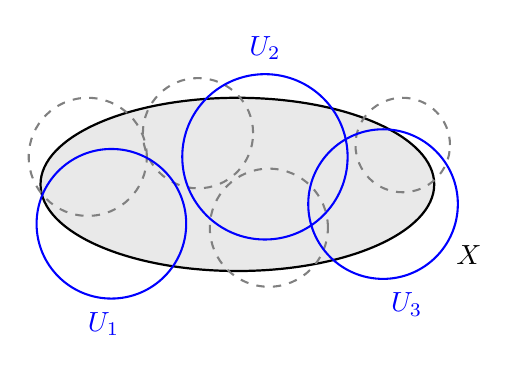
\begin{tikzpicture}[scale=1.0]
    \draw[thick, fill=lightgray, fill opacity=0.35] (0,0) ellipse (2.5 and 1.1);
    \node[anchor=west] at (2.65,-0.9) {$X$};
    \draw[color=gray, dash pattern={on 3pt off 3pt}] (-1.9,0.35) circle (0.75);
    \draw[color=gray, dash pattern={on 3pt off 3pt}] (-0.5,0.65) circle (0.7);
    \draw[color=gray, dash pattern={on 3pt off 3pt}] (0.4,-0.55) circle (0.75);
    \draw[color=gray, dash pattern={on 3pt off 3pt}] (2.1,0.5) circle (0.6);
    \draw[color=blue] (-1.6,-0.5) circle (0.95);
    \draw[color=blue] (0.35,0.35) circle (1.05);
    \draw[color=blue] (1.85,-0.25) circle (0.95);
    \node[color=blue, anchor=north] at (-1.7,-1.5) {$U_1$};
    \node[color=blue, anchor=south] at (0.35,1.45) {$U_2$};
    \node[color=blue, anchor=north] at (2.15,-1.25) {$U_3$};
\end{tikzpicture}
\end{center}

The picture: out of a possibly enormous open cover (dashed), we can always select finitely many sets (solid) which still cover a compact space.

The motivating discussion above proves most of the following theorem.

\begin{theorem}[Boundedness and the Extreme Value Theorem]\label{thm:evt}
    Let $X$ be a compact topological space and $f: X \rightarrow \R$ continuous. Then $f$ is bounded, and if $X \neq \emptyset$ then $f$ attains its bounds.
\end{theorem}
\begin{proof}
    For boundedness, cover $X$ by the open sets $U_n = \{x \mid |f(x)| < n\}$ for $n \in \N$ (open as preimages of open intervals). By compactness finitely many suffice, and since the $U_n$ are nested, $X = U_N$ for some $N$, so $|f| < N$ on $X$.

    Now suppose $X \neq \emptyset$, and let $\alpha = \inf_X f$, which exists as $f$ is bounded. Suppose for contradiction that $f(x) > \alpha$ for all $x \in X$. Then the open sets
    $$
    V_n = f^{-1}\left(\left(\alpha + \tfrac{1}{n}, \infty\right)\right), \quad n \in \N
    $$
    cover $X$, so again by compactness and nestedness, $X = V_N$ for some $N$. But then $f(x) > \alpha + \frac{1}{N}$ for all $x$, so $\inf_X f \geq \alpha + \frac{1}{N} > \alpha$, a contradiction. The supremum is attained by applying this to $-f$.
\end{proof}

Of course, all this is only useful if we have a good supply of compact spaces. The fundamental example is the closed bounded interval.

\begin{theorem}[{$[0, 1]$ is Compact}]\label{thm:01compact}
    The closed interval $[0, 1]$ is compact.
\end{theorem}
\begin{proof}
    Let $\mathcal{U}$ be a family of open sets in $\R$ covering $[0, 1]$. Say that $\mathcal{U}$ \emph{finitely covers} a set $A \subset [0, 1]$ if finitely many members of $\mathcal{U}$ cover $A$; note that if $A = B \cup C$ and $\mathcal{U}$ finitely covers $B$ and $C$, then it finitely covers $A$.

    Suppose $\mathcal{U}$ does not finitely cover $[0, 1]$. Bisecting, at least one of $[0, \frac{1}{2}]$ and $[\frac{1}{2}, 1]$ is not finitely covered; call it $[a_1, b_1]$. Bisecting again and repeating, we get nested intervals
    $$
    [0,1] \supset [a_1, b_1] \supset [a_2, b_2] \supset \cdots, \quad b_n - a_n = 2^{-n},
    $$
    none of which is finitely covered by $\mathcal{U}$. The sequence $a_n$ is increasing and bounded, so $a_n \rightarrow x$ for some $x \in [0, 1]$, and $b_n = a_n + 2^{-n} \rightarrow x$ too.

    Since $\mathcal{U}$ covers $[0, 1]$, there's some $U \in \mathcal{U}$ with $x \in U$, and since $U$ is open, $(x - \varepsilon, x + \varepsilon) \subset U$ for some $\varepsilon > 0$. But for large enough $n$, both $a_n$ and $b_n$ lie in $(x - \varepsilon, x + \varepsilon)$, so $[a_n, b_n] \subset U$ is covered by the single set $U$ -- contradicting that $[a_n, b_n]$ is not finitely covered.
\end{proof}

\begin{example}[Compact and Non-Compact Spaces]
    \begin{enumerate}[label=(\roman*)]
        \item Any finite topological space is compact, as is any set with the indiscrete or cofinite topology\footnote{For the cofinite topology: pick any non-empty $U$ in the cover; its complement is finite, and each missing point needs only one more set.}.
        \item If $x_n \rightarrow x$ in a topological space, then $\{x_n \mid n \in \N\} \cup \{x\}$ is compact: any cover contains some $U \ni x$, which contains all but finitely many of the $x_n$, and finitely many more sets mop up the rest.
        \item An infinite discrete space is not compact: the cover by singletons has no finite subcover.
        \item $\R$ is not compact: the cover by the intervals $(-n, n)$ for $n \in \N$ has no finite subcover. Similarly $(0, 1]$ is not compact, using the cover $(1/n, 2)$ for $n \in \N$ -- note how this cover exploits the `missing' endpoint $0$.
    \end{enumerate}
\end{example}

\subsection{Building New Compact Spaces}

The next two results tell us how compactness interacts with subspaces, and they display a pleasing duality between `compact' and `closed'.

\begin{theorem}[Compactness and Closed Subspaces]\label{thm:compactclosed}
    Let $Y$ be a subspace of a topological space $X$.
    \begin{enumerate}[label=(\roman*)]
        \item If $X$ is compact and $Y$ is closed in $X$, then $Y$ is compact.
        \item If $X$ is Hausdorff and $Y$ is compact, then $Y$ is closed in $X$.
    \end{enumerate}
\end{theorem}
\begin{proof}
    \emph{Part (i)}. Let $\mathcal{U}$ be a family of open sets of $X$ covering $Y$. Since $Y$ is closed, $\mathcal{U} \cup \{X \backslash Y\}$ is an open cover of $X$, which by compactness has a finite subcover. Discarding $X \backslash Y$ from it if present, we are left with finitely many members of $\mathcal{U}$ covering $Y$.

    \emph{Part (ii)}. We show $X \backslash Y$ is open. Let $x \in X \backslash Y$. For each $y \in Y$, using the Hausdorff property pick disjoint open sets $U_y \ni x$ and $V_y \ni y$. The $V_y$ cover $Y$, so by compactness there is a finite $F \subset Y$ with $Y \subset \bigcup_{y \in F} V_y$. Then
    $$
    U = \bigcap_{y \in F} U_y
    $$
    is a finite intersection of open sets, so open, contains $x$, and misses every $V_y$ for $y \in F$, hence misses $Y$. So $X \backslash Y$ is a neighborhood of each of its points, and $Y$ is closed.
\end{proof}

Note that part (ii) genuinely needs the Hausdorff hypothesis: in an infinite indiscrete space, every subset is compact, but only $\emptyset$ and the whole space are closed.

\begin{theorem}[Continuous Images of Compact Spaces]\label{thm:ctsimage}
    Let $f: X \rightarrow Y$ be a continuous function between topological spaces. If $X$ is compact, then $f(X)$ is compact.
\end{theorem}
\begin{proof}
    Let $\mathcal{U}$ be a family of open sets in $Y$ covering $f(X)$. Then $\{f^{-1}(U) \mid U \in \mathcal{U}\}$ is an open cover of $X$, so finitely many $f^{-1}(U_1), \dots, f^{-1}(U_k)$ cover $X$, and then $U_1, \dots, U_k$ cover $f(X)$.
\end{proof}

So compactness is a topological property, and any quotient of a compact space is compact. Also, combining with Theorem~\ref{thm:01compact}: any closed interval $[a, b] \cong [0, 1]$ is compact, and Theorem~\ref{thm:evt} recovers the familiar extreme value theorem of Analysis I.

Here is a first genuinely topological payoff. Recall that a continuous bijection need not have a continuous inverse -- but compactness fixes this.

\begin{theorem}[Topological Inverse Function Theorem]\label{thm:topift}
    Let $f: X \rightarrow Y$ be a continuous bijection from a compact space $X$ to a Hausdorff space $Y$. Then $f^{-1}$ is continuous, and hence $f$ is a homeomorphism.
\end{theorem}
\begin{proof}
    It's enough to show $f$ is an open map, or equivalently (taking complements, $f$ being a bijection) that $f$ maps closed sets to closed sets. So let $K \subset X$ be closed. Since $X$ is compact, $K$ is compact; hence $f(K)$ is compact as a continuous image; hence $f(K)$ is closed in $Y$, since $Y$ is Hausdorff. Done -- notice how the previous two theorems slotted together perfectly.
\end{proof}

\begin{example}[$\R/\Z \cong S^1$]
    We can now deliver on our promise from the section on quotients: $\R/\Z$ is homeomorphic to the circle
    $$
    S^1 = \{v \in \R^2 \mid \norm{v} = 1\}.
    $$
    Define $f: \R \rightarrow S^1$ by $f(t) = (\cos 2\pi t, \sin 2\pi t)$. Then $f$ is continuous (its components are), surjective, and $f(s) = f(t)$ if and only if $s - t \in \Z$, so $f$ fully respects the relation defining $\R/\Z$. By our results on quotients, $f$ descends to a continuous bijection $\tilde{f}: \R/\Z \rightarrow S^1$.

    Now, $\R/\Z = q([0, 1])$ is the image of a compact space under the (continuous) quotient map, so it is compact. Also $S^1$ is a metric space, hence Hausdorff. So $\tilde{f}$ is a continuous bijection from a compact space to a Hausdorff space, and by the topological inverse function theorem, it is a homeomorphism.
\end{example}

Next, products. The general form of this theorem -- for infinite products -- is a famous and much deeper result of Tychonov, but for finite products the proof is a pleasant exercise in cover manipulation.

\begin{theorem}[Tychonov's Theorem, Finite Case]\label{thm:tychonov}
    If $X$ and $Y$ are compact topological spaces, then $X \times Y$ is compact.
\end{theorem}
\begin{proof}
    Let $\mathcal{U}$ be an open cover of $X \times Y$. We first reduce to covers by boxes: each $z \in X \times Y$ lies in some $W_z \in \mathcal{U}$, and by the definition of the product topology there are open $U_z, V_z$ with $z \in U_z \times V_z \subset W_z$. If finitely many of the boxes $U_z \times V_z$ cover $X \times Y$, then the corresponding $W_z$ form a finite subcover of $\mathcal{U}$. So we may assume every member of $\mathcal{U}$ is a box $U \times V$.

    Fix $x \in X$. The slice $\{x\} \times Y$ is the continuous image of $Y$ (under $y \mapsto (x, y)$), so it is compact, and it is covered by $\mathcal{U}$. Hence there are finitely many boxes
    $$
    U_{x, 1} \times V_{x, 1}, \; \dots, \; U_{x, n_x} \times V_{x, n_x} \in \mathcal{U}
    $$
    covering $\{x\} \times Y$, and we may discard any that don't actually meet the slice, so that $x \in U_{x, j}$ for each $j$. Now let
    $$
    U_x = \bigcap_{j = 1}^{n_x} U_{x, j},
    $$
    an open set containing $x$. The key point is that the same finite family covers the whole `tube' over $U_x$:
    $$
    U_x \times Y \subset \bigcup_{j = 1}^{n_x} U_{x, j} \times V_{x, j},
    $$
    since for $(u, y) \in U_x \times Y$, the point $(x, y)$ lies in some $U_{x, j} \times V_{x, j}$, and then $(u, y)$ does too as $u \in U_x \subset U_{x,j}$.

    Finally, $\{U_x \mid x \in X\}$ is an open cover of the compact space $X$, so $X = \bigcup_{x \in F} U_x$ for some finite $F \subset X$. Then
    $$
    X \times Y = \bigcup_{x \in F} U_x \times Y \subset \bigcup_{x \in F} \bigcup_{j = 1}^{n_x} U_{x, j} \times V_{x, j},
    $$
    a finite subcover.
\end{proof}

By induction, any finite product of compact spaces is compact. Combining everything, we arrive at the definitive description of the compact subsets of Euclidean space.

\begin{theorem}[Heine-Borel]
    A subset $K \subset \R^n$ is compact if and only if $K$ is closed and bounded.
\end{theorem}
\begin{proof}
    Suppose $K$ is compact. $\R^n$ is a metric space, hence Hausdorff, so $K$ is closed by Theorem~\ref{thm:compactclosed}. And $x \mapsto \norm{x}$ is continuous, so it is bounded on $K$ by Theorem~\ref{thm:evt}, which says exactly that $K$ is bounded.

    Conversely, suppose $K$ is closed and bounded, say $\norm{x} \leq M$ for all $x \in K$. Then $K \subset [-M, M]^n$. Each $[-M, M]$ is compact (being homeomorphic to $[0, 1]$), so $[-M, M]^n$ is compact by Tychonov, and $K$ is a closed subset of it, hence compact.
\end{proof}

\begin{example}
    Closed balls $B_r(x)$ in $\R^n$ are compact, as are spheres. And we can finally tie up a loose end from the proof of the Picard-Lindel\"of theorem: a continuous function on $[a, b] \times B_R(y_0) \subset \R^{n+1}$ is bounded, since its domain is closed and bounded, hence compact.
\end{example}

\subsection{Sequential Compactness}

In metric spaces we made heavy use of the Bolzano-Weierstrass property -- every bounded sequence has a convergent subsequence. There is a corresponding abstract notion.

\begin{definition}[Sequentially Compact]
    A topological space $X$ is \vocab{sequentially compact} if every sequence in $X$ has a subsequence converging to a point of $X$.
\end{definition}

It will be convenient to have some notation: given a sequence $x_n$ and an infinite subset $M = \{m_1 < m_2 < \cdots\} \subset \N$, we write $(x_m)_{m \in M}$ for the subsequence $x_{m_1}, x_{m_2}, \dots$. Note that if $L \subset M$ are infinite, then $(x_m)_{m \in L}$ is a subsequence of $(x_m)_{m \in M}$.

\begin{example}[Bolzano-Weierstrass in $\R^n$]\label{ex:bwrn}
    Any closed bounded subset $K \subset \R^n$ is sequentially compact. Indeed, let $x_m = (x_{m, 1}, \dots, x_{m, n})$ be a sequence in $K$; each coordinate sequence is bounded. By Bolzano-Weierstrass applied to the first coordinate, there's an infinite $M_1 \subset \N$ such that $(x_{m, 1})_{m \in M_1}$ converges. The second coordinate restricted to $M_1$ is still bounded, so there's an infinite $M_2 \subset M_1$ with $(x_{m, 2})_{m \in M_2}$ convergent -- and note the first coordinate still converges along $M_2$. Continuing, we get $M_n \subset \cdots \subset M_1$ such that all coordinates converge along $M_n$, so $(x_m)_{m \in M_n}$ converges in $\R^n$, with limit in $K$ since $K$ is closed.
\end{example}

So for subsets of $\R^n$, sequential compactness and compactness agree (both are `closed and bounded'). This is no accident: we will now show that they agree in \emph{every} metric space. (For general topological spaces the two notions genuinely diverge -- there are compact spaces that are not sequentially compact and vice versa -- but the examples are exotic and beyond this course.)

We will actually prove a three-way equivalence, bringing in completeness as well. The third notion we need is a strengthening of boundedness.

\begin{definition}[Totally Bounded]
    Let $(M, d)$ be a metric space. For $\varepsilon > 0$, a subset $F \subset M$ is an \vocab{$\varepsilon$-net} for $M$ if
    $$
    M = \bigcup_{y \in F} B_{\varepsilon}(y),
    $$
    that is, every point of $M$ is within $\varepsilon$ of some point of $F$. We say $M$ is \vocab{totally bounded} if for every $\varepsilon > 0$ there is a \emph{finite} $\varepsilon$-net for $M$.
\end{definition}

Totally bounded implies bounded, but not conversely: an infinite set with the discrete metric is bounded but has no finite $\frac{1}{2}$-net. Similarly the closed unit ball of $\ell_\infty(\N)$ is bounded but not totally bounded.

\begin{definition}[Diameter]
    For a non-empty subset $A$ of a metric space, the \vocab{diameter} of $A$ is $\diam A = \sup\{d(x, y) \mid x, y \in A\}$.
\end{definition}

\begin{lemma}[Chopping Up a Totally Bounded Space]\label{lemma:chop}
    Let $M$ be a totally bounded metric space, let $A \subset M$ be non-empty and closed, and let $\varepsilon > 0$. Then we can write $A = B_1 \cup \cdots \cup B_K$ where each $B_k$ is non-empty and closed with $\diam B_k \leq \varepsilon$.
\end{lemma}
\begin{proof}
    Let $F$ be a finite $\frac{\varepsilon}{2}$-net for $M$, so that $A = \bigcup_{x \in F} (A \cap B_{\varepsilon/2}(x))$. Throw away the $x$ for which the intersection is empty, and for the rest let $B_x = A \cap B_{\varepsilon/2}(x)$. Each $B_x$ is non-empty, closed (an intersection of closed sets), has $\diam B_x \leq \diam B_{\varepsilon/2}(x) \leq \varepsilon$, and together they cover $A$.
\end{proof}

\begin{theorem}[The Big Equivalence]\label{thm:bigequiv}
    For a metric space $(M, d)$, the following are equivalent:
    \begin{enumerate}[label=(\roman*)]
        \item $M$ is compact;
        \item $M$ is sequentially compact;
        \item $M$ is complete and totally bounded.
    \end{enumerate}
\end{theorem}
\begin{proof}
    \emph{(i) implies (ii)}. Let $x_n$ be a sequence in $M$, and for each $n$ let $T_n = \{x_k \mid k > n\}$ be its $n$-th tail. We first claim $\bigcap_{n} \ol{T_n} \neq \emptyset$. If not, then the open sets $M \backslash \ol{T_n}$ cover $M$, so by compactness finitely many do; since the $T_n$ are decreasing, this means $M = M \backslash \ol{T_N}$ for some $N$, that is, $\ol{T_N} = \emptyset$ -- absurd, since $T_N \neq \emptyset$.

    So pick $x \in \bigcap_n \ol{T_n}$. Since $x \in \ol{T_1}$, the ball $D_1(x)$ meets $T_1$, so there is $k_1 > 1$ with $d(x_{k_1}, x) < 1$. Since $x \in \ol{T_{k_1}}$, the ball $D_{1/2}(x)$ meets $T_{k_1}$, giving $k_2 > k_1$ with $d(x_{k_2}, x) < \frac{1}{2}$. Continuing inductively, we get $k_1 < k_2 < \cdots$ with $d(x_{k_n}, x) < \frac{1}{n}$, so $x_{k_n} \rightarrow x$.

    \emph{(ii) implies (iii)}. For completeness, let $x_n$ be Cauchy, and use sequential compactness to extract a subsequence $x_{k_n} \rightarrow x$. Given $\varepsilon > 0$, take $N$ so that $d(x_m, x_n) < \varepsilon$ for $m, n \geq N$. For fixed $n \geq N$, since $k_m \geq m$,
    $$
    d(x_n, x) \leq d(x_n, x_{k_m}) + d(x_{k_m}, x) \leq \varepsilon + d(x_{k_m}, x) \rightarrow \varepsilon
    $$
    as $m \rightarrow \infty$. So $d(x_n, x) \leq \varepsilon$ for all $n \geq N$, and $x_n \rightarrow x$.

    For total boundedness, suppose it fails for some $\varepsilon > 0$: no finite set is an $\varepsilon$-net. Then we can inductively pick $x_1 \in M$ and
    $$
    x_n \in M \backslash \bigcup_{j = 1}^{n - 1} B_{\varepsilon}(x_j),
    $$
    since the union on the right never covers $M$. The resulting sequence has $d(x_m, x_n) > \varepsilon$ for all $m \neq n$, so it has no Cauchy subsequence, and hence no convergent subsequence -- contradicting sequential compactness.

    \emph{(iii) implies (i)}. Let $\mathcal{U}$ be an open cover of $M$, and suppose for contradiction that no finite subfamily covers $M$. We construct a nested sequence of `bad' sets: let $A_0 = M$, and suppose we have found a non-empty closed $A_{n - 1}$ which is not finitely covered by $\mathcal{U}$. By Lemma~\ref{lemma:chop} we can write $A_{n - 1}$ as a finite union of non-empty closed sets of diameter at most $\frac{1}{n}$; if each piece were finitely covered, so would $A_{n-1}$ be, so some piece is not finitely covered -- call it $A_n$. This gives non-empty closed sets
    $$
    M = A_0 \supset A_1 \supset A_2 \supset \cdots, \quad \diam A_n \leq \tfrac{1}{n},
    $$
    with no $A_n$ finitely covered by $\mathcal{U}$.

    Now pick $x_n \in A_n$ for each $n$. For $m, n \geq N$ both $x_m, x_n$ lie in $A_N$, so $d(x_m, x_n) \leq \frac{1}{N}$, and the sequence is Cauchy. By completeness $x_n \rightarrow x$ for some $x \in M$; since each $A_N$ is closed and contains the tail of the sequence, $x \in A_N$ for every $N$. Take $U \in \mathcal{U}$ with $x \in U$ and $r > 0$ with $D_r(x) \subset U$. Choosing $n$ with $d(x_n, x) < \frac{r}{2}$ and $\diam A_n < \frac{r}{2}$, every $y \in A_n$ satisfies
    $$
    d(y, x) \leq d(y, x_n) + d(x_n, x) < \tfrac{r}{2} + \tfrac{r}{2} = r,
    $$
    so $A_n \subset D_r(x) \subset U$. But then $A_n$ is covered by the single set $U \in \mathcal{U}$, contradicting that it is not finitely covered.
\end{proof}

\begin{remark}
    Note that (iii) makes the slogan `compact = complete + totally bounded' precise: compactness is completeness plus an approximate finiteness. It also explains why compactness is such a strong hypothesis in analysis. As sanity checks: combining Example~\ref{ex:bwrn} with the theorem re-proves the hard direction of Heine-Borel from Bolzano-Weierstrass, and one can also check directly that a finite product of sequentially compact spaces is sequentially compact, giving an alternative proof of Tychonov's theorem for metric spaces.
\end{remark}

As a final application, we can deliver on a promise made back in our study of uniform continuity: the Bolzano-Weierstrass argument we used there works verbatim on any compact metric space.

\begin{theorem}[Heine-Cantor]
    Let $f: M \rightarrow M'$ be a continuous map between metric spaces, with $M$ compact. Then $f$ is uniformly continuous.
\end{theorem}
\begin{proof}
    If not, there is some $\varepsilon > 0$ such that for every $n$ we can find $x_n, y_n \in M$ with $d(x_n, y_n) < \frac{1}{n}$ but $d'(f(x_n), f(y_n)) \geq \varepsilon$. By sequential compactness, passing to a subsequence we may assume $x_n \rightarrow x \in M$, and then $y_n \rightarrow x$ too since $d(x_n, y_n) \rightarrow 0$. By continuity, $f(x_n) \rightarrow f(x)$ and $f(y_n) \rightarrow f(x)$, so
    $$
    d'(f(x_n), f(y_n)) \leq d'(f(x_n), f(x)) + d'(f(x), f(y_n)) \rightarrow 0,
    $$
    contradicting $d'(f(x_n), f(y_n)) \geq \varepsilon$.
\end{proof}

\section{Differentiation from $\R^m$ to $\R^n$}

For the final part of the course, we return from the abstract world of topological spaces to concrete multivariable analysis, and develop the theory of differentiation for functions $f: \R^m \rightarrow \R^n$. The metric and topological machinery we've built -- open sets, completeness, connectedness, the contraction mapping theorem -- will all earn its keep here.

\subsection{The Derivative as a Linear Map}

What should it mean for $f: \R^m \rightarrow \R^n$ to be differentiable at a point? The one-dimensional definition,
$$
f'(a) = \lim_{h \to 0} \frac{f(a + h) - f(a)}{h},
$$
doesn't directly generalize -- we can't divide by a vector $h \in \R^m$. The right move is to reformulate. In one dimension, $f$ is differentiable at $a$ with derivative $\lambda$ if and only if
$$
f(a + h) = f(a) + \lambda h + h\varepsilon(h),
$$
where $\varepsilon(h) \rightarrow 0$ as $h \rightarrow 0$. Read this way, the derivative is not really a number -- it's the \emph{linear map} $h \mapsto \lambda h$ which best approximates the change in $f$ near $a$. Linear maps make perfect sense between $\R^m$ and $\R^n$, and this is the definition that generalizes.

Before making this precise, we need a tiny bit of setup about the space of linear maps itself. Write $L(\R^m, \R^n)$ for the vector space of linear maps $T: \R^m \rightarrow \R^n$. Fixing standard bases $e_1, \dots, e_m$ of $\R^m$ and $e_1', \dots, e_n'$ of $\R^n$, each $T$ is represented by the $n \times m$ matrix with entries $T_{ji} = \langle Te_i, e_j' \rangle$, so $L(\R^m, \R^n)$ can be identified with $\R^{nm}$, and we give it the Euclidean norm
$$
\norm{T} = \left(\sum_{i = 1}^m \sum_{j = 1}^n T_{ji}^2\right)^{1/2} = \left( \sum_{i = 1}^m \norm{Te_i}^2 \right)^{1/2}.
$$
In particular $L(\R^m, \R^n)$ is a metric space with $d(S, T) = \norm{S - T}$, and everything we know about $\R^{nm}$ (completeness, Heine-Borel, and so on) applies to it.

\begin{lemma}[Linear Maps are Lipschitz]\label{lemma:linlip}
    For $T \in L(\R^m, \R^n)$ and $x \in \R^m$ we have $\norm{Tx} \leq \norm{T} \norm{x}$. Consequently every linear map is Lipschitz, hence continuous. Moreover, for $S \in L(\R^n, \R^p)$ we have $\norm{ST} \leq \norm{S}\norm{T}$.
\end{lemma}
\begin{proof}
    Writing $x = \sum_i x_i e_i$, we have $Tx = \sum_i x_i \, Te_i$, so by the triangle inequality and Cauchy-Schwarz,
    $$
    \norm{Tx} \leq \sum_{i = 1}^m |x_i| \norm{Te_i} \leq \left(\sum_{i = 1}^m x_i^2\right)^{1/2} \left(\sum_{i = 1}^m \norm{Te_i}^2\right)^{1/2} = \norm{x} \norm{T}.
    $$
    Then $\norm{Tx - Ty} = \norm{T(x - y)} \leq \norm{T}\norm{x - y}$, so $T$ is Lipschitz. Finally,
    $$
    \norm{ST} = \left(\sum_{i = 1}^m \norm{S(Te_i)}^2\right)^{1/2} \leq \left(\sum_{i = 1}^m \norm{S}^2\norm{Te_i}^2\right)^{1/2} = \norm{S} \norm{T}. \qedhere
    $$
\end{proof}

Now we can make our main definition. We work on open subsets, since differentiability at $a$ should only depend on the behaviour of $f$ near $a$.

\begin{definition}[Differentiability]
    Let $U \subset \R^m$ be open, $f: U \rightarrow \R^n$ and $a \in U$. We say $f$ is \vocab{differentiable at $a$} if there exists a linear map $T \in L(\R^m, \R^n)$ such that
    $$
    \frac{f(a + h) - f(a) - T(h)}{\norm{h}} \rightarrow 0 \quad \text{as } h \rightarrow 0.
    $$
    Equivalently, $f(a + h) = f(a) + T(h) + \norm{h}\, \varepsilon(h)$, where $\varepsilon(h) \rightarrow 0 = \varepsilon(0)$ as $h \rightarrow 0$.

    If $f$ is differentiable at every point of $U$, we say $f$ is \vocab{differentiable on $U$}.
\end{definition}

\begin{proposition}[Uniqueness of the Derivative]
    The linear map $T$ in the definition above is unique.
\end{proposition}
\begin{proof}
    Suppose $S$ and $T$ both work. Subtracting the two conditions gives
    $$
    \frac{S(h) - T(h)}{\norm{h}} \rightarrow 0 \quad \text{as } h \rightarrow 0.
    $$
    Fix $x \neq 0$ and take $h = x/k$ for $k \in \N$, so $h \rightarrow 0$ as $k \rightarrow \infty$. By linearity, $(S(h) - T(h))/\norm{h}$ doesn't depend on $k$ at all -- it always equals $(S(x) - T(x))/\norm{x}$. So this quantity is $0$, and $S(x) = T(x)$ for all $x$.
\end{proof}

We call this unique $T$ the \vocab{derivative} of $f$ at $a$, and write $f'(a) = Df(a) = T$. So $f'(a)$ is a \emph{linear map} $\R^m \rightarrow \R^n$, and the defining property is
$$
f(a + h) = f(a) + f'(a)(h) + o(\norm{h}),
$$
where as usual $o(\norm{h})$ denotes a quantity which, divided by $\norm{h}$, tends to $0$ as $h \rightarrow 0$. The right picture is that the affine function $x \mapsto f(a) + f'(a)(x - a)$ is the \emph{best linear approximation} to $f$ near $a$ -- its graph is the tangent line (or plane) to the graph of $f$, and the error dies off faster than linearly.

\begin{center}
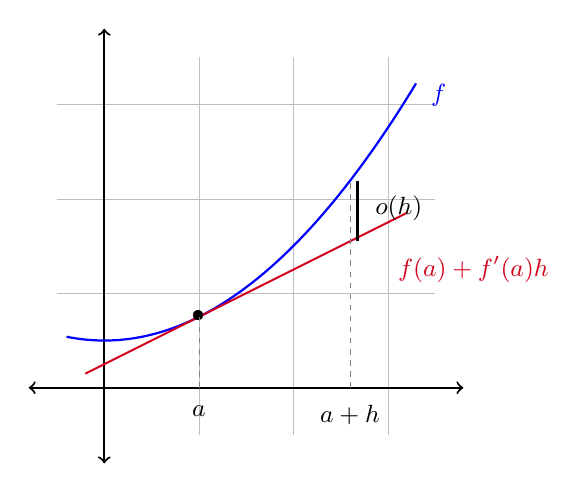
\begin{tikzpicture}[scale=1.2]
    \draw[ultra thin, color=lightgray] (-0.5,-0.5) grid (3.5,3.5);
    \draw[<->] (-0.8,0) -- (3.8,0);
    \draw[<->] (0,-0.8) -- (0,3.8);
    \draw[thick, samples=100, smooth, domain=-0.4:3.3, color=blue] plot (\x, {0.25*(\x)^2 + 0.5});
    \draw[color={rgb,255:red,208;green,2;blue,27}, domain=-0.2:3.2] plot (\x, {0.5*\x + 0.25});
    \node[color=blue, anchor=west] at (3.35,3.1) {\small $f$};
    \node at (1,0.75) {\textbullet};
    \node[anchor=north] at (1,-0.08) {\small $a$};
    \draw[ultra thin, color=gray, dash pattern={on 2pt off 2pt}] (1,0) -- (1,0.75);
    \draw[ultra thin, color=gray, dash pattern={on 2pt off 2pt}] (2.6,0) -- (2.6,2.19);
    \node[anchor=north] at (2.6,-0.08) {\small $a + h$};
    \draw[thick, color=black] (2.68,1.55) -- (2.68,2.19);
    \node[anchor=west] at (2.76,1.9) {\small $o(\norm{h})$};
    \node[color={rgb,255:red,208;green,2;blue,27}, anchor=north west] at (3.0,1.5) {\small $f(a) + f'(a)h$};
\end{tikzpicture}
\end{center}

\begin{remark}[Recovering the One-Dimensional Derivative]
    When $m = 1$, a linear map $\R \rightarrow \R^n$ is just multiplication by a fixed vector $v \in \R^n$, and the condition becomes $(f(a + h) - f(a))/h \rightarrow v$: the familiar limit definition, now taking vector values. So for curves, the derivative-as-linear-map and the derivative-as-vector are the same information.
\end{remark}

Let's compute some derivatives from the definition.

\begin{example}[Constant and Linear Maps]
    If $f(x) = b$ is constant, then $f(a + h) = f(a) + 0(h) + 0$, so $f$ is differentiable with $f'(a) = 0$ for all $a$.

    If $f(x) = Tx$ for a fixed $T \in L(\R^m, \R^n)$, then $f(a + h) = f(a) + T(h) + 0$, so $f'(a) = T$ for every $a$ -- a linear map is its own best linear approximation, everywhere.
\end{example}

\begin{example}[The Norm-Squared Function]
    Let $f: \R^m \rightarrow \R$ be $f(x) = \norm{x}^2$. Then
    $$
    f(a + h) = \norm{a}^2 + 2\langle a, h\rangle + \norm{h}^2 = f(a) + 2\langle a, h \rangle + o(\norm{h}),
    $$
    since $\norm{h}^2/\norm{h} = \norm{h} \rightarrow 0$. The map $h \mapsto 2\langle a, h\rangle$ is linear, so $f$ is differentiable with $f'(a)(h) = 2\langle a, h\rangle$.
\end{example}

\begin{example}[Squaring a Matrix]
    Let $M_n$ denote the space of $n \times n$ real matrices, identified with $\R^{n^2}$, and let $f: M_n \rightarrow M_n$ be $f(A) = A^2$. Then
    $$
    f(A + H) = A^2 + AH + HA + H^2,
    $$
    and $H \mapsto AH + HA$ is linear, while $\norm{H^2} \leq \norm{H}^2 = o(\norm{H})$ using Lemma~\ref{lemma:linlip}. So $f'(A)(H) = AH + HA$. (For $n = 1$ this is the statement that the derivative of $x^2$ is multiplication by $2x$ -- but note that for $n > 1$ we cannot collapse $AH + HA$ to $2AH$, as matrices don't commute.)
\end{example}

As in one dimension, differentiability is stronger than continuity.

\begin{proposition}[Differentiable Implies Continuous]
    If $f: U \rightarrow \R^n$ is differentiable at $a \in U$, then $f$ is continuous at $a$.
\end{proposition}
\begin{proof}
    Write $f(x) = f(a) + f'(a)(x - a) + \norm{x - a}\,\varepsilon(x - a)$. As $x \rightarrow a$: the middle term tends to $0$ since linear maps are continuous, and the error term tends to $0$. So $f(x) \rightarrow f(a)$.
\end{proof}

The chain rule survives intact, and in fact its statement becomes cleaner than in one dimension: the derivative of a composition is the \emph{composition} of the derivatives.

\begin{theorem}[Chain Rule]
    Let $U \subset \R^m$ and $V \subset \R^n$ be open, and let $f: U \rightarrow \R^n$ and $g: V \rightarrow \R^p$ with $f(U) \subset V$. If $f$ is differentiable at $a$ and $g$ is differentiable at $b = f(a)$, then $g \circ f$ is differentiable at $a$, with
    $$
    (g \circ f)'(a) = g'(b) \circ f'(a).
    $$
\end{theorem}
\begin{proof}
    Write $S = f'(a)$ and $T = g'(b)$, so that
    $$
    f(a + h) = f(a) + S(h) + \norm{h}\varepsilon(h), \quad g(b + k) = g(b) + T(k) + \norm{k}\zeta(k),
    $$
    with $\varepsilon(h) \rightarrow 0$ and $\zeta(k) \rightarrow 0$. Substituting $k = k(h) = S(h) + \norm{h}\varepsilon(h)$,
    \begin{align*}
        (g \circ f)(a + h) &= g(b + k) = g(b) + T(S(h) + \norm{h}\varepsilon(h)) + \norm{k}\zeta(k) \\
        &= (g \circ f)(a) + (T \circ S)(h) + \underbrace{\norm{h}\, T(\varepsilon(h)) + \norm{k} \zeta(k)}_{\eta(h)}.
    \end{align*}
    It remains to show $\eta(h) = o(\norm{h})$. For the first piece, $\norm{T(\varepsilon(h))} \leq \norm{T}\norm{\varepsilon(h)} \rightarrow 0$. For the second, note
    $$
    \frac{\norm{k}}{\norm{h}} \leq \frac{\norm{S(h)} + \norm{h}\norm{\varepsilon(h)}}{\norm{h}} \leq \norm{S} + \norm{\varepsilon(h)},
    $$
    which is bounded for small $h$; and $k \rightarrow 0$ as $h \rightarrow 0$, so $\zeta(k) \rightarrow 0$. Hence
    $$
    \frac{\norm{\eta(h)}}{\norm{h}} \leq \norm{T(\varepsilon(h))} + \frac{\norm{k}}{\norm{h}}\norm{\zeta(k)} \rightarrow 0,
    $$
    as required.
\end{proof}

Just as for continuity, differentiability can be checked component by component.

\begin{proposition}[Components]\label{prop:components}
    Let $U \subset \R^m$ be open, $f: U \rightarrow \R^n$, and write $f_j = \pi_j \circ f$ for the components of $f$, where $\pi_j: \R^n \rightarrow \R$ is the $j$-th coordinate projection. Then $f$ is differentiable at $a$ if and only if every $f_j$ is, and in that case
    $$
    f'(a)(h) = \sum_{j = 1}^n f_j'(a)(h) \, e_j'.
    $$
\end{proposition}
\begin{proof}
    If $f$ is differentiable at $a$, then since $\pi_j$ is linear (so differentiable, and equal to its own derivative), the chain rule gives $f_j'(a) = \pi_j \circ f'(a)$, which is the claim. Conversely, if each $f_j$ is differentiable at $a$, write $f_j(a + h) = f_j(a) + f_j'(a)(h) + \norm{h}\varepsilon_j(h)$; summing against $e_j'$,
    $$
    f(a + h) = f(a) + \sum_{j = 1}^n f_j'(a)(h)e_j' + \norm{h}\sum_{j = 1}^n \varepsilon_j(h) e_j',
    $$
    and the final error term is $o(\norm{h})$ since each $\varepsilon_j(h) \rightarrow 0$.
\end{proof}

This is a very useful reduction -- it means that in many proofs we may assume $n = 1$ without loss of generality. Finally, the usual algebraic rules.

\begin{proposition}[Sums and Products]
    Let $U \subset \R^m$ be open and let $f, g: U \rightarrow \R^n$ and $\phi: U \rightarrow \R$ all be differentiable at $a \in U$. Then $f + g$ and $\phi f$ are differentiable at $a$, with
    $$
    (f + g)'(a) = f'(a) + g'(a), \quad (\phi f)'(a)(h) = \phi(a) f'(a)(h) + \left[\phi'(a)(h)\right] f(a).
    $$
\end{proposition}
\begin{proof}
    The sum rule follows immediately by adding the two defining expansions. For the product, expanding $\phi(a + h)f(a + h)$ using both expansions gives
    $$
    (\phi f)(a) + \phi(a)f'(a)(h) + \phi'(a)(h)f(a) + \rho(h),
    $$
    where $\rho(h)$ collects the remaining terms: $\phi'(a)(h) \cdot f'(a)(h)$, and various products involving an error term. The first satisfies $\norm{\phi'(a)(h)f'(a)(h)} \leq \norm{\phi'(a)}\norm{f'(a)}\norm{h}^2 = o(\norm{h})$, and the rest are also $o(\norm{h})$ since each contains a factor $\norm{h}$ (or a bounded multiple of it) alongside a factor tending to zero. The map $h \mapsto \phi(a)f'(a)(h) + \phi'(a)(h)f(a)$ is linear, so the result follows. Taking $m = n = 1$ recovers the familiar product rule.
\end{proof}

\subsection{Partial Derivatives}

The definition of the derivative is clean, but to \emph{compute} with it we want to reduce to one-dimensional derivatives. This is what directional and partial derivatives do.

\begin{definition}[Directional and Partial Derivatives]
    Let $U \subset \R^m$ be open, $f: U \rightarrow \R^n$, $a \in U$, and let $u \in \R^m$ be non-zero. If the limit
    $$
    D_u f(a) = \lim_{t \to 0} \frac{f(a + tu) - f(a)}{t}
    $$
    exists (in $\R^n$), we call it the \vocab{directional derivative} of $f$ at $a$ in the direction $u$.

    When $u = e_i$ is a standard basis vector, we write $D_i f(a) = D_{e_i} f(a)$ and call it the \vocab{$i$-th partial derivative} of $f$ at $a$. For scalar components we use the familiar notation $D_i f_j(a) = \frac{\partial f_j}{\partial x_i}(a)$.
\end{definition}

Note that $D_u f(a)$ is exactly the derivative at $0$ of the one-variable function $t \mapsto f(a + tu)$ -- we restrict $f$ to a line through $a$ and differentiate along it.

\begin{proposition}[The Derivative Determines All Directional Derivatives]\label{prop:dirderiv}
    If $f$ is differentiable at $a$, then $D_u f(a)$ exists for every direction $u \neq 0$, and
    $$
    D_u f(a) = f'(a)(u).
    $$
    In particular, writing $h = \sum_i h_i e_i$,
    $$
    f'(a)(h) = \sum_{i = 1}^m h_i D_i f(a),
    $$
    so the derivative is determined by the $m$ partial derivatives.
\end{proposition}
\begin{proof}
    Setting $h = tu$ in the definition of differentiability,
    $$
    \frac{f(a + tu) - f(a)}{t} = f'(a)(u) + \frac{|t|}{t}\norm{u} \, \varepsilon(tu),
    $$
    and the error term tends to $0$ as $t \rightarrow 0$ (the factor $|t|/t$ is bounded). The second claim follows from linearity of $f'(a)$.
\end{proof}

\begin{definition}[Jacobian Matrix]
    If $f$ is differentiable at $a$, the matrix of $f'(a)$ with respect to the standard bases is called the \vocab{Jacobian matrix} $J_f(a)$. By the proposition, its $i$-th column is $D_i f(a)$, so its entries are
    $$
    (J_f(a))_{ji} = D_i f_j(a) = \frac{\partial f_j}{\partial x_i}(a).
    $$
\end{definition}

It is important that the converse of Proposition~\ref{prop:dirderiv} fails: a function can have all directional derivatives at a point without being differentiable there.

\begin{example}[Directional Derivatives Are Not Enough]
    Define $f: \R^2 \rightarrow \R$ by
    $$
    f(x, y) = \frac{x^3}{x^2 + y^2} \text{ for } (x, y) \neq (0,0), \quad f(0, 0) = 0.
    $$
    For any direction $u = (u_1, u_2)$, we have
    $$
    \frac{f(tu) - f(0)}{t} = \frac{1}{t}\cdot\frac{t^3u_1^3}{t^2 u_1^2 + t^2u_2^2} = \frac{u_1^3}{\norm{u}^2},
    $$
    so all directional derivatives at the origin exist (and equal this value). But $u \mapsto u_1^3/\norm{u}^2$ is \emph{not linear} in $u$, so by Proposition~\ref{prop:dirderiv}, $f$ cannot be differentiable at the origin.
\end{example}

However, if the partial derivatives exist \emph{near} $a$ and are continuous \emph{at} $a$, then we do get differentiability. This is the workhorse criterion for checking differentiability in practice.

\begin{theorem}[Continuous Partials Imply Differentiability]\label{thm:c1diff}
    Let $U \subset \R^m$ be open, $f: U \rightarrow \R^n$, and $a \in U$. Suppose there is an open neighborhood $V \subset U$ of $a$ on which all partial derivatives $D_i f$ exist, and that each $D_i f: V \rightarrow \R^n$ is continuous at $a$. Then $f$ is differentiable at $a$.
\end{theorem}
\begin{proof}
    By Proposition~\ref{prop:components} we may assume $n = 1$. We also present the proof for $m = 2$ -- the general case works in exactly the same way, one coordinate at a time, at the cost of heavier notation. Write $a = (p, q)$, and let
    $$
    \psi(h, k) = f(p + h, q + k) - f(p, q) - hD_1f(p, q) - kD_2f(p, q).
    $$
    We must show $\psi(h, k) = o(\norm{(h,k)})$; then $f$ is differentiable at $a$ with derivative $(h, k) \mapsto hD_1f(a) + kD_2f(a)$. The trick is to move from $(p, q)$ to $(p + h, q + k)$ one coordinate at a time:
    $$
    \psi(h, k) = \underbrace{\left[f(p + h, q + k) - f(p + h, q) - kD_2f(p, q)\right]}_{(1)} + \underbrace{\left[f(p + h, q) - f(p, q) - hD_1f(p, q)\right]}_{(2)}.
    $$
    Term $(2)$ is $o(|h|)$, hence $o(\norm{(h, k)})$, directly by the definition of $D_1 f(p, q)$.

    For term $(1)$, fix $h, k$ small and consider $\phi(t) = f(p + h, q + tk)$ for $t \in [0, 1]$. Then $\phi$ is differentiable with $\phi'(t) = k \, D_2 f(p + h, q + tk)$, so by the one-dimensional mean value theorem there's some $\theta = \theta(h, k) \in (0, 1)$ with
    $$
    f(p + h, q + k) - f(p + h, q) = \phi(1) - \phi(0) = k\,D_2f(p + h, q + \theta k).
    $$
    Hence term $(1)$ equals $k\left[D_2f(p + h, q + \theta k) - D_2f(p, q)\right]$. As $(h, k) \rightarrow 0$, the point $(p + h, q + \theta k) \rightarrow (p, q)$, so by continuity of $D_2 f$ at $a$, the bracket tends to $0$, and term $(1)$ is $o(|k|) = o(\norm{(h,k)})$.
\end{proof}

\begin{definition}[$C^1$ Function]
    Let $U \subset \R^m$ be open. A function $f: U \rightarrow \R^n$ is \vocab{$C^1$ on $U$} (or \vocab{continuously differentiable}) if $f$ is differentiable on $U$ and the derivative map $f': U \rightarrow L(\R^m, \R^n)$ is continuous.
\end{definition}

Since the entries of the Jacobian are the partial derivatives, and convergence in $L(\R^m, \R^n) \cong \R^{nm}$ is entry-wise, $f$ is $C^1$ on $U$ if and only if all partial derivatives $D_if_j$ exist and are continuous on $U$ -- combining Theorem~\ref{thm:c1diff} with Proposition~\ref{prop:dirderiv}.

\subsection{The Mean Value Inequality}

The mean value \emph{theorem} -- that $f(b) - f(a) = f'(c)(b - a)$ for some intermediate $c$ -- fails for vector-valued functions; different components want different intermediate points\footnote{Consider $f(t) = (\cos t, \sin t)$: we have $f(2\pi) - f(0) = 0$, but $f'$ never vanishes.}. But in analysis we almost always used the mean value theorem to \emph{bound} increments, and the bound survives beautifully.

\begin{theorem}[Mean Value Inequality]\label{thm:mvi}
    Let $U \subset \R^m$ be open and $f: U \rightarrow \R^n$ differentiable on $U$. Suppose $a, b \in U$ are such that the segment $[a, b] = \{(1 - t)a + tb \mid t \in [0, 1]\}$ lies in $U$, and that $\norm{f'(z)} \leq M$ for all $z \in [a, b]$. Then
    $$
    \norm{f(b) - f(a)} \leq M\norm{b - a}.
    $$
\end{theorem}
\begin{proof}
    Let $u = b - a$ (we may assume $u \neq 0$) and let $v = f(b) - f(a)$. The trick is to convert to a scalar problem by projecting onto $v$: define
    $$
    \phi(t) = \langle f(a + tu), v\rangle, \quad t \in [0, 1].
    $$
    By the chain rule (composing $t \mapsto a + tu$ with $f$, then with the linear map $\langle \cdot, v \rangle$), $\phi$ is differentiable with
    $$
    \phi'(t) = \langle f'(a + tu)(u), v\rangle.
    $$
    By the one-dimensional mean value theorem, there's some $\theta \in (0, 1)$ with $\phi(1) - \phi(0) = \phi'(\theta)$. But $\phi(1) - \phi(0) = \langle f(b) - f(a), v\rangle = \norm{v}^2$, so by Cauchy-Schwarz and Lemma~\ref{lemma:linlip},
    $$
    \norm{v}^2 = \langle f'(a + \theta u)(u), v\rangle \leq \norm{f'(a + \theta u)}\norm{u}\norm{v} \leq M \norm{b - a} \norm{v}.
    $$
    If $v = 0$ there is nothing to prove; otherwise divide by $\norm{v}$.
\end{proof}

Here is the promised payoff from connectedness.

\begin{corollary}[Zero Derivative Implies Constant]
    Let $U \subset \R^m$ be open and \emph{connected}, and let $f: U \rightarrow \R^n$ be differentiable with $f'(a) = 0$ for all $a \in U$. Then $f$ is constant.
\end{corollary}
\begin{proof}
    For any $x \in U$, take $r > 0$ with $D_r(x) \subset U$. The ball is convex, so for $y \in D_r(x)$ the segment $[x, y]$ lies in $U$, and the mean value inequality with $M = 0$ gives $f(y) = f(x)$. So $f$ is \emph{locally constant}.

    Now fix $x_0 \in U$ and let $P = \{x \in U \mid f(x) = f(x_0)\}$. By local constancy, both $P$ and $U \backslash P$ are open. Since $U$ is connected and $P \ni x_0$ is non-empty, we must have $P = U$.
\end{proof}

Note that connectedness is genuinely needed -- on a disconnected open set, a function can be constant on each piece with different values.

\subsection{Second Derivatives}

If $f: U \rightarrow \R^n$ is differentiable on $U$, its derivative is itself a function $f': U \rightarrow L(\R^m, \R^n)$ into the (finite dimensional, normed) space of linear maps, and we can ask for \emph{its} derivative.

\begin{definition}[Second Derivative]
    Let $U \subset \R^m$ be open, $f: U \rightarrow \R^n$, and $a \in U$. Suppose $f$ is differentiable on some open neighborhood $V \subset U$ of $a$. We say $f$ is \vocab{twice differentiable at $a$} if $f': V \rightarrow L(\R^m, \R^n)$ is differentiable at $a$, and write $f''(a)$ for its derivative, so
    $$
    f''(a) \in L(\R^m, L(\R^m, \R^n)).
    $$
\end{definition}

An element of $L(\R^m, L(\R^m, \R^n))$ is awkward to think about directly, but there is a standard way out: such a gadget is the same thing as a \emph{bilinear map} $\R^m \times \R^m \rightarrow \R^n$. Explicitly, if $T \in L(\R^m, L(\R^m, \R^n))$, we identify it with the bilinear map $(h, k) \mapsto T(h)(k)$, and we will freely write $f''(a)(h, k)$ for $\left(f''(a)(h)\right)(k)$.

\begin{proposition}[Second Derivative as a Bilinear Approximation]
    In the setting above, $f$ is twice differentiable at $a$ if and only if there is a bilinear map $T: \R^m \times \R^m \rightarrow \R^n$ such that for every fixed $k \in \R^m$,
    $$
    f'(a + h)(k) = f'(a)(k) + T(h, k) + o(\norm{h}) \quad \text{as } h \rightarrow 0,
    $$
    and in that case $T = f''(a)$.
\end{proposition}
\begin{proof}
    If $f$ is twice differentiable at $a$, then $f'(a + h) = f'(a) + f''(a)(h) + \norm{h}\varepsilon(h)$ where $\varepsilon(h) \rightarrow 0$ in $L(\R^m, \R^n)$. Evaluating at $k$ and using $\norm{\varepsilon(h)(k)} \leq \norm{\varepsilon(h)}\norm{k} \rightarrow 0$ gives the displayed formula.

    Conversely, suppose the formula holds for each fixed $k$, and let
    $$
    \varepsilon(h) = \frac{f'(a + h) - f'(a) - T(h)}{\norm{h}} \in L(\R^m, \R^n).
    $$
    By hypothesis $\varepsilon(h)(k) \rightarrow 0$ for each fixed $k$; taking $k = e_1, \dots, e_m$ and using
    $$
    \norm{\varepsilon(h)} = \left(\sum_{i = 1}^m \norm{\varepsilon(h)(e_i)}^2\right)^{1/2} \rightarrow 0,
    $$
    we get $\varepsilon(h) \rightarrow 0$ in $L(\R^m, \R^n)$, which is twice differentiability with $f''(a) = T$.
\end{proof}

\begin{example}
    If $f$ is linear then $f'$ is the constant function $a \mapsto f$, so $f''(a) = 0$ everywhere. If $f: \R^m \times \R^n \rightarrow \R^p$ is \emph{bilinear}, then a similar computation to the matrix-squaring example shows $f'(a, b)(h, k) = f(a, k) + f(h, b)$, which is \emph{linear} as a function of $(a, b)$ -- so $f''$ is constant, equal to the bilinear map $((h,k),(h',k')) \mapsto f(h, k') + f(h', k)$.
\end{example}

\begin{example}[Cubing a Matrix]
    Let $f: M_n \rightarrow M_n$ be $f(A) = A^3$. Expanding $(A + H)^3$ and collecting terms of degree $1$ in $H$,
    $$
    f'(A)(H) = A^2H + AHA + HA^2,
    $$
    with the degree-$\geq 2$ terms being $o(\norm{H})$. Then expanding $f'(A + H)(K) - f'(A)(K)$ and collecting the terms linear in $H$,
    $$
    f''(A)(H, K) = AHK + HAK + AKH + HKA + KAH + KHA,
    $$
    which is indeed bilinear in $(H, K)$, and symmetric under swapping $H$ and $K$. In one dimension these formulas collapse to the familiar $f'(a) = 3a^2$ and $f''(a) = 6a$.
\end{example}

The symmetry visible in that example is no coincidence. To see what it means concretely, evaluate the second derivative on directions: if $f$ is twice differentiable at $a$, then for fixed $v$, the map $x \mapsto D_v f(x) = f'(x)(v)$ is differentiable at $a$, and by the proposition above,
$$
D_u D_v f(a) = (D_vf)'(a)(u) = f''(a)(u, v).
$$
In particular $D_iD_jf(a) = f''(a)(e_i, e_j)$: second partial derivatives are the entries of the second derivative.

\begin{theorem}[Symmetry of Second Derivatives]
    Let $U \subset \R^m$ be open, $f: U \rightarrow \R^n$, and $a \in U$. Suppose $f$ is twice differentiable on an open $V$ with $a \in V \subset U$, and that $f'': V \rightarrow \operatorname{Bil}(\R^m \times \R^m, \R^n)$ is continuous at $a$. Then for all $u, v$,
    $$
    f''(a)(u, v) = f''(a)(v, u),
    $$
    that is, $f''(a)$ is a symmetric bilinear map. Equivalently, $D_uD_vf(a) = D_vD_uf(a)$.
\end{theorem}
\begin{proof}
    Considering components (which commute with everything in sight), we may assume $n = 1$. The key object is the \emph{second difference}
    $$
    \phi(s, t) = f(a + su + tv) - f(a + tv) - f(a + su) + f(a),
    $$
    for small $s, t > 0$ -- the alternating sum of $f$ over the vertices of the parallelogram spanned by $su$ and $tv$. It is manifestly symmetric between the roles of $(s, u)$ and $(t, v)$, and we will compute its size in two ways.

    Fix $s, t$ and let $\psi(y) = f(a + yu + tv) - f(a + yu)$, so that $\phi(s, t) = \psi(s) - \psi(0)$. By the mean value theorem, there's some $\alpha \in (0, 1)$ with
    $$
    \phi(s, t) = s\psi'(\alpha s) = s\left[D_uf(a + \alpha su + tv) - D_uf(a + \alpha su)\right].
    $$
    Applying the mean value theorem again, to $y \mapsto D_uf(a + \alpha su + yv)$, gives $\beta \in (0, 1)$ with
    $$
    \phi(s, t) = st\, D_vD_uf(a + \alpha su + \beta tv) = st\,f''(a + \alpha su + \beta tv)(v, u).
    $$
    Since $f''$ is continuous at $a$, letting $s, t \rightarrow 0$ gives
    $$
    \frac{\phi(s, t)}{st} \rightarrow f''(a)(v, u).
    $$
    But by symmetry of $\phi$, running the same argument with $\psi(y) = f(a + su + yv) - f(a + yv)$ instead gives
    $$
    \frac{\phi(s, t)}{st} \rightarrow f''(a)(u, v).
    $$
    Limits are unique, so $f''(a)(u, v) = f''(a)(v, u)$.
\end{proof}

\begin{remark}
    Taking $u = e_i$, $v = e_j$, this is the familiar statement that mixed partial derivatives commute,
    $$
    \frac{\partial^2 f}{\partial x_i \partial x_j}(a) = \frac{\partial^2 f}{\partial x_j \partial x_i}(a),
    $$
    for (say) twice continuously differentiable $f$ -- so for scalar $f$, the \emph{Hessian matrix} $(D_iD_jf(a))_{ij}$ is symmetric. Some continuity hypothesis is genuinely needed; without it there are standard counterexamples where the two mixed partials at a point disagree.
\end{remark}

\subsection{The Inverse Function Theorem}

We finish the course with a genuine highlight -- a theorem that combines nearly everything we have done: completeness and the contraction mapping theorem, open sets and continuity, the mean value inequality, and the derivative as a linear map.

The question is: when does a function $f$ have a differentiable inverse? There is an obvious necessary condition. If $f: V \rightarrow W$ is a bijection between open sets, differentiable at $a$ with differentiable inverse $g$ at $f(a)$, then differentiating $g \circ f = \operatorname{id}$ and $f \circ g = \operatorname{id}$ with the chain rule shows that $g'(f(a)) \circ f'(a)$ and $f'(a) \circ g'(f(a))$ are both identity maps -- so $f'(a)$ must be an \emph{invertible} linear map\footnote{Taking traces of the two identities also shows $m = n$: differentiably-invertible maps only exist between spaces of equal dimension.}.

The inverse function theorem says that, for $C^1$ functions, this necessary condition is \emph{locally sufficient}: wherever the derivative is invertible, the function itself is invertible near that point, with $C^1$ inverse.

\begin{theorem}[Inverse Function Theorem]
    Let $U \subset \R^n$ be open and $f: U \rightarrow \R^n$ a $C^1$ function. Let $a \in U$ and suppose $f'(a)$ is invertible. Then there exist open sets $V \ni a$ and $W \ni f(a)$, with $V \subset U$, such that $f|_V: V \rightarrow W$ is a bijection, and its inverse $g: W \rightarrow V$ is $C^1$ with
    $$
    g'(y) = \left[f'(g(y))\right]^{-1} \quad \text{for all } y \in W.
    $$
\end{theorem}

\begin{center}
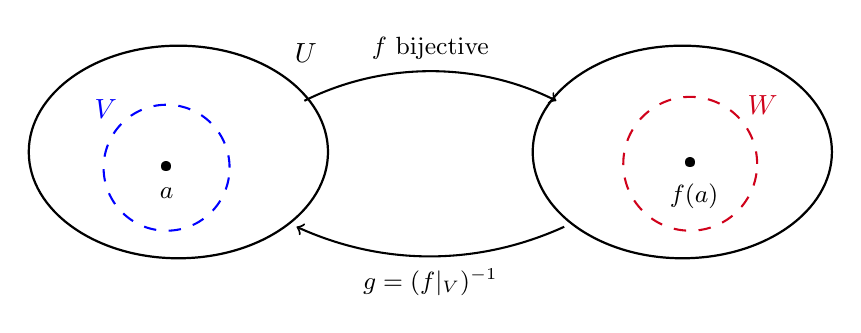
\begin{tikzpicture}[scale=1.0]
    \draw[thick] (-3.2,0.1) ellipse (1.9 and 1.35);
    \node[anchor=south west] at (-1.85,1.1) {$U$};
    \draw[color=blue, dash pattern={on 4.5pt off 4.5pt}] (-3.35,-0.1) circle (0.8);
    \node at (-3.35,-0.1) {\textbullet};
    \node[anchor=north] at (-3.35,-0.22) {\small $a$};
    \node[color=blue, anchor=east] at (-3.85,0.65) {$V$};
    \draw[thick] (3.2,0.1) ellipse (1.9 and 1.35);
    \draw[color={rgb,255:red,208;green,2;blue,27}, dash pattern={on 4.5pt off 4.5pt}] (3.3,-0.05) circle (0.85);
    \node at (3.3,-0.05) {\textbullet};
    \node[anchor=north] at (3.35,-0.17) {\small $f(a)$};
    \node[color={rgb,255:red,208;green,2;blue,27}, anchor=west] at (3.9,0.7) {$W$};
    \draw[->] (-1.6,0.75) .. controls (-0.6,1.25) and (0.6,1.25) .. (1.6,0.75);
    \node[anchor=south] at (0,1.15) {\small $f$ bijective};
    \draw[<-] (-1.7,-0.85) .. controls (-0.6,-1.35) and (0.6,-1.35) .. (1.7,-0.85);
    \node[anchor=north] at (0,-1.25) {\small $g = (f|_V)^{-1}$};
\end{tikzpicture}
\end{center}

\begin{proof}
    We proceed in several steps.

    \emph{Step 0: normalisation.} We first argue that we may assume $a = 0$, $f(a) = 0$ and $f'(a) = I$, the identity map. Indeed, let $T = f'(a)$ and set
    $$
    h(x) = T^{-1}\left(f(x + a) - f(a)\right),
    $$
    defined on the open set $U - a \ni 0$. By the chain rule (linear maps being their own derivatives), $h$ is differentiable with $h'(x) = T^{-1} \circ f'(x + a)$, so $h(0) = 0$ and $h'(0) = I$; moreover
    $$
    \norm{h'(x) - h'(y)} \leq \norm{T^{-1}}\norm{f'(x + a) - f'(y + a)},
    $$
    so $h$ is also $C^1$. If the theorem holds for $h$, then it holds for $f$, since $f(x) = T(h(x - a)) + f(a)$ and composing with the fixed homeomorphisms $x \mapsto x - a$, $y \mapsto T(y) + f(a)$ (whose derivatives are invertible) transports all the conclusions back. So assume $f(0) = 0$ and $f'(0) = I$.

    \emph{Step 1: $f$ doesn't collapse distances near $0$.} Since $f'$ is continuous, there is $r > 0$ such that $B_r(0) \subset U$ and
    $$
    \norm{f'(x) - I} \leq \tfrac{1}{2} \quad \text{for all } x \in B_r(0).
    $$
    Consider $p(x) = f(x) - x$, so $p'(x) = f'(x) - I$ has $\norm{p'(x)} \leq \frac{1}{2}$ on $B_r(0)$. The ball is convex, so the mean value inequality gives, for $x, y \in B_r(0)$,
    $$
    \norm{p(x) - p(y)} \leq \tfrac{1}{2}\norm{x - y},
    $$
    and hence
    $$
    \norm{f(x) - f(y)} \geq \norm{x - y} - \norm{p(x) - p(y)} \geq \tfrac{1}{2}\norm{x - y}.
    $$
    In particular $f$ is injective on $B_r(0)$.

    \emph{Step 2: $f$ hits everything near $0$.} Let $s = r/2$. We claim that for every $w \in D_s(0)$ there is a unique $x \in D_r(0)$ with $f(x) = w$. Fix such a $w$ and define
    $$
    q(x) = w - p(x) = w - f(x) + x,
    $$
    so that $f(x) = w$ if and only if $q(x) = x$: solving our equation means finding a fixed point of $q$. Now for $x \in B_r(0)$, using $p(0) = 0$,
    $$
    \norm{q(x)} \leq \norm{w} + \norm{p(x) - p(0)} < s + \tfrac{1}{2}\norm{x} \leq \tfrac{r}{2} + \tfrac{r}{2} = r,
    $$
    so $q$ maps $B_r(0)$ into $D_r(0) \subset B_r(0)$. Moreover, for $x, y \in B_r(0)$,
    $$
    \norm{q(x) - q(y)} = \norm{p(x) - p(y)} \leq \tfrac{1}{2}\norm{x - y},
    $$
    so $q$ is a contraction of the non-empty \emph{complete} metric space $B_r(0)$ (closed and bounded in $\R^n$, hence complete). By the contraction mapping theorem, $q$ has a unique fixed point $x \in B_r(0)$, and since $q$ maps into the open ball, in fact $x \in D_r(0)$. This proves the claim.

    \emph{Step 3: the local inverse, and its continuity.} Let
    $$
    W = D_s(0), \quad V = D_r(0) \cap f^{-1}(W).
    $$
    Then $W$ is open, and $V$ is open as an intersection of open sets ($f$ being continuous), with $0 \in V$. By Step 2, $f|_V: V \rightarrow W$ is a bijection; call its inverse $g: W \rightarrow V$. For $u, v \in W$, writing $x = g(u)$, $y = g(v)$, Step 1 gives
    $$
    \norm{g(u) - g(v)} = \norm{x - y} \leq 2\norm{f(x) - f(y)} = 2\norm{u - v},
    $$
    so $g$ is $2$-Lipschitz, and in particular continuous.

    \emph{Step 4: differentiability of the inverse.} First note that for $x \in B_r(0)$, the linear map $f'(x)$ is invertible: if $f'(x)v = 0$ then
    $$
    \norm{v} = \norm{(I - f'(x))v} \leq \norm{I - f'(x)}\norm{v} \leq \tfrac{1}{2}\norm{v},
    $$
    so $v = 0$, and an injective linear map $\R^n \rightarrow \R^n$ is invertible.

    Now fix $y \in W$ and let $x = g(y) \in V$, $S = f'(x)$. Let $k$ be small enough that $y + k \in W$, and set $h = g(y + k) - g(y)$, so that $f(x + h) = y + k$ and, by the Lipschitz bound on $g$, $\norm{h} \leq 2\norm{k}$. Differentiability of $f$ at $x$ gives
    $$
    k = f(x + h) - f(x) = S(h) + \norm{h}\varepsilon(h), \quad \varepsilon(h) \rightarrow 0 \text{ as } h \rightarrow 0.
    $$
    Applying $S^{-1}$,
    $$
    g(y + k) - g(y) - S^{-1}(k) = h - S^{-1}(S(h) + \norm{h}\varepsilon(h)) = -\norm{h}\, S^{-1}(\varepsilon(h)),
    $$
    and hence
    $$
    \frac{\norm{g(y + k) - g(y) - S^{-1}(k)}}{\norm{k}} \leq \frac{\norm{h}}{\norm{k}}\norm{S^{-1}}\norm{\varepsilon(h)} \leq 2\norm{S^{-1}}\norm{\varepsilon(h)}.
    $$
    As $k \rightarrow 0$ we have $h \rightarrow 0$ (continuity of $g$), so the right hand side tends to $0$. This shows $g$ is differentiable at $y$ with
    $$
    g'(y) = S^{-1} = \left[f'(g(y))\right]^{-1}.
    $$

    Finally, $g'$ is continuous: it is the composition of the continuous maps $g$ (Step 3), $f'$ (as $f$ is $C^1$), and matrix inversion, which is continuous on the set of invertible matrices since the entries of $A^{-1}$ are rational functions (with non-vanishing denominator $\det A$) of the entries of $A$. So $g$ is $C^1$, completing the proof.
\end{proof}

\begin{remark}
    A couple of closing remarks on this theorem.
    \begin{enumerate}[label=(\roman*)]
        \item The conclusion is genuinely \emph{local}. The map $f: \R^2 \rightarrow \R^2$ given in complex notation by $z \mapsto e^z$ has everywhere-invertible derivative, and is locally invertible near every point, but it is not injective globally (as $e^{z + 2\pi i} = e^z$).
        \item The inverse function theorem is the gateway to the \emph{implicit function theorem} and to the theory of manifolds and submanifolds -- it is the tool that lets us straighten out nonlinear maps locally, and it will reappear throughout courses in differential geometry and analysis.
    \end{enumerate}
\end{remark}

